\documentclass[]{article}
\usepackage[utf8]{inputenc}
\usepackage[spanish]{babel}
\usepackage{graphicx}
\usepackage{vmargin}
\usepackage{fancyhdr}
\usepackage{float}

%\cfoot{\textit{\thepage}} 

\setpapersize{A4}
\setmargins{2.5cm}       % margen izquierdo
{1.5cm}                        % margen superior
{16.5cm}                      % anchura del texto
{23.42cm}                    % altura del texto
{10pt}                           % altura de los encabezados
{1cm}                           % espacio entre el texto y los encabezados
{0pt}                             % altura del pie de página
{2cm}                           % espacio entre el texto y el pie de página

%opening
\title{Apuntes para preparar \textsc{Green Belt}}
\author{Nicolás Rodríguez Lucena}

\begin{document}


\maketitle

\part{Introducción}
\section{Six Sigma y metas organizativas}

\begin{quote}
	\textbf{Six Sigma busca reducir la variación y mejorar el control del proceso.}
\end{quote}
\begin{quote}
\textbf{Lean expulsa residuos y promueve el estandarizar trabajos.}
\end{quote}

En una organización, todos los que están envueltos en ella, quieren y necesitan que el negocio satisfaga de una manera eficiente y que se consigan las metas. Esta es la filosofía Lean Six Sigma.
Motorola fomenta el Six Sigma a finales de los 80. General Electric de primeras se muestra reticente pero en los 90 comienza a desarrollarse en esta filosofía. Son las dos compañías que lanzan la filoosfía de la mejora contínua. El fracaso más común en cualquier corporación es la falta de compromiso por parte de la dirección frente a la mejora real de los procesos.

\textit{Advanced quality planning (AQP)} es la herramienta utilizada en la gestión para hacer la implementación de Six Sigma en organizaciones. Así empiezan los gestores a tomar decisiones basadas en los datos y a desplegar el sistema.

La especialidad \textit{Quality Control/Quality Assurance (QC/QA)} se creó para asegurar que los estándares eran establecidos y mantenidos para la satisfacción del cliente. La evolución ha llevado a quitar al experto QC/QA la responsabilidad del sistema sobre la satisfacción de cliente, pasando a ser incluida en todos los miembros de la organización. 

\begin{center}
	\line(1,0){250}
\end{center}

\textbf{Shewhart} utilizó gráficos para monitorizar procesos y detectar causas especiales que desviaran los resultados de lo esperado (\textit{quality control charts, process behavior charts}).

Ford en 1988 lanzó el programa \textit{supplier quality improvement (SQI)} para trabajar con proveedores externos en nuevos diseños de vehículos utilizando los \textit{advanced quality planning (AQP)} de la ASQ para mejorar la calidad en el ensamblaje, y todo esto dio lugar al \textit{advanced product quality planning (APQP)} que se utiliza actualmente en la industria automotriz. 

Motorola le presentó el Six Sigma a Ford y lo evaluó contra Ford Q1 y Q-101 (precursor de ISO/TS 16949). Solo un punto que no le gustó, estaba establecido el $C_p$ en 1.0. Ford quería $C_{pk} >$ 1.33 para procesos conocidos y $C_{pk} >$ 1.67 para los nuevos.

\begin{center}
	\line(1,0){250}
\end{center}

\textbf{Chowdhury}: trabaja en la línea de que los problemas pueden ser evitados a través de la mejora continua, la calidad es responsabilidad de todos, la calidad empieza en la dirección, todos tienen un papel en la calidad, la calidad es el balance entre el poder de la gente y del proceso. Poder de la gente necesita compromiso, honestidad y empatía. El poder del proceso es sobre solucionar problemas, desarrollar ideas y soluciones. Toda organización es única, cada individuo trae diferente conocimiento y habilidades. Métodos y procesos deben ser desarrollados para cada específica situación.

\begin{center}
	\line(1,0){250}
\end{center}

\textbf{Philip Crosby}: Desarrolló sus 14 pasos. 
\begin{itemize} \item 1) Gerencia comprometida con la calidad \item 2) Los equipos de mejora continua deben tener miembros de todos los departamentos \item 3) Determinar como medir donde están los problemas actuales \item 4) Evaluar el coste de calidad y explicar su uso como herramienta de gestión \item 5) Incrementar la conciencia de calidad en la organización \item 6) Tomar acciones formales para corregir problemas identificados en pasos anteriores \item 7) Poner un comité de 0-defectos \item 8) Formación para todos \item 9) Establecer el día 0-defectos \item 10) Alentar a que la gente establezca metas de mejora para ellos y para sus grupos \item 11) Alentar a la gente a que comente los problemas de gestión \item 12) Reconocer y apreciar la participación de la gente \item 13) Establecer ``Consejos de Calidad'' para comunicarse de manera regular. \item 14) Re-ejecutar el programa desde 0 una vez terminado, para que la gente vea que esto nunca se acaba. 
	\end{itemize}
\begin{center}
	\line(1,0){250}
\end{center}
\textbf{W. Edwards Deming}: Otros 14 puntos. 
\begin{itemize} \item 1) Constancia en la mejora \item  2) Nueva filosofía \item  3) No todo es inspección  \item 4) No todo es precio \item  5) Mejora constante para planificación, producción y servicio \item 6) Formación \item 7) Liderazgo \item 8) Evitar miedos \item 9) Quitar barreras entre el staff \item 10) Fuera el trabajo duro \item 11) Eliminar cuotas para cuantificar trabajo duro y metas numéricas para la gestión \item 12) Quitar barreras que roben a la gente el orgullo del trabajo. Fuera sistemas de méritos etc... \item 13) Plan de Formación y mejora personal \item 14) Todos en la organización para realizar el cambio. \end{itemize}  Y sus 7 enfermedades mortales: \begin{itemize} \item 1) Falta de constancia \item 2) El cortoplacismo \item 3) Evaluación por méritos \item 4) Movilidad de la gestión \item 5) El funcionamiento basado solo en 'figuras visibles' \item 6) Costes médicos excesivos \item 7) Costes excesivos de garantía, alimentados por abogados que trabajan por honorarios. \end{itemize}

También preparó el \textit{Sistema del conocimiento profundo}: 1) Apreciación de un sistema (\textit{process aproach}) 2) Conocimiento de la variación (existe, cómo reconocerla). 3) Teoría del conocimiento (\textit{how to learn}) 4) Conocimiento de la psicología (Maslow, Regla de Platino...) 
\begin{center}
	\line(1,0){250}
\end{center}
\textbf{Armand Feigenbaum}: Planifica y transmite el plan. Planificar es algo positivo, necesario y que da valor ya que el propósito de la planificación es ``hacer las cosas bien''. En tres pasos: Liderazgo de la calidad, tecnología moderna de la calidad y comité de organización. Los planes AQP son de su autoría. 
\begin{center}
	\line(1,0){250}
\end{center}
\textbf{Kaoru Ishikawa}: Diagrama causa-efecto. Trabajó con Deming estrechamente. Sus puntos: Calidad primero, por delante de rentabilidad cortoplacista. Orientar hacia cliente, pensar desde su POV. Destaca la necesidad de que haya \textit{feedback} con cliente. La gestión de mejora debe basarse en hechos y datos, estadística. Respeto a la gente como filosofía de gestión. Gestión interfuncional. Sus contribuciones clave: los círculos de calidad japoneses, el diagrama \textit{fishbone}, el desarrollo de control de calidad amigable y el centrarse en los clientes internos.
\begin{center}
	\line(1,0){250}
\end{center}
\textbf{Joseph M Juran}: \textit{Quality planning, quality control} y \textit{quality improvement}. Sus puntos clave: crear conciencia sobre la mejora, la calidad es de todos, haz una infraestructura de calidad (\textit{consejos, nombrar equipos, ...}), formación sobre Calidad, revisiones periódicas, reconocimiento a los equipos ganadores, propagandizar los resultados, revisar el sistema de recompensas para hacer cumplir el ratio de mejoras, mantener un plan de negocio basado en la mejora de la calidad. Pareto es suyo. 
\begin{center}
	\line(1,0){250}
\end{center}
\textbf{Dorian Shainin}: Ing. aeronáutico que desarrolla soluciones para los problemas mas difíciles. Habla con las \textit{partes}, son mas listas que los ingenieros. Desarrolló herramientas estadísticas las cuales se llamaron Red X.
\begin{center}
	\line(1,0){250}
\end{center}
\textbf{Walter Shewhart} trabajador de Western Electric inventó el PDCA y es el padre del control estadístico de proceso. 
\begin{center}
	\line(1,0){250}
\end{center}
\textbf{D. H. Stamatis}: 45 libros sobre Six Sigma, calidad y demás. Su Manual del FMEA \textit{de la teoría a la práctica} es considerado el origen del FMEA para la industria.
\begin{center}
	\line(1,0){250}
\end{center}
\textbf{Genichi Taguchi}: Inventó la Loss Function, usada para medir el coste financiero por empeorar la calidad y desarrolló la filosofía de \textit{off-line quality control}. 
\begin{center}
	\line(1,0){250}
\end{center}
\textbf{Proceso}: serie de pasos diseñada para producir productos o servicios. A menudo representado como un diagrama de flujo con \textit{inputs} (materiales, recursos, info), \textit{steps}, y \textit{outputs}. 

Six Sigma está incluido en el círculo DMAIC (\textit{define, measure, analyze, improve y control}), utilizado para gestionar problemas.

\textbf{Business Systems}: diseñados para implementar un conjunto de procesos. Se asegura de que todo esté en el lugar adecuado en el momento adecuado. Tiene como meta la mejora continua de procesos, productos y servicios. Se encarga de recoger y analizar la información de los procesos y de otras fuentes para la mejora continua. \newline
Hay dos maneras de ver el método. Una, utilizando inputs / recursos para producir resultados de \textbf{calidad}: la gestión de procesos es recoger datos y analizarlo, aplicando el \textit{feedback} al proceso. Por otro lado se piensa que el proceso debe ser diseñado orientado hacia la \textbf{colección de datos}, análisis y el \textit{feedback} que se va a producir.

\textbf{Las 7M en Six Sigma}: \textit{Man, Machine, Methods, Mother Nature, Management, Materials, Measurement System} para Productos y/o Servicios. \newline Métodos alternativos al Six Sigma: Quality Operating System (QoS), mejora continua (CI), \textit{total quality management} (TQM), mejora de procesos (PI). Todos comparten el mismo reto: revisar procesos para mejoras: mantenimientos preventivos, limpieza, desgaste... \newline La línea general es: qué medir, cómo medirlo, saber si es fundamental el proceso, tener un consenso sobre defectos, exponer defectos latentes, observar la calidad estadística (cartas de comportamiento de proceso) y distinguir entre Calidad de Diseño y Calidad de Conformidad. 

\subsection{Modelo DMAIC}
Define: PDCA, SIPOC, 5W, Systems thinking, Process Identification, Flowchart, Project Management.

Measure: PDCA, Data Collection Plan, Measurement Systems Analysis (MSA), Collect Data (check sheets, Histograms, Pareto Charts, Scatter Diagrams), identificar variabilidad-instabilidad, Benchmark, Start Cost of Quality. 

Analyze: PD\textbf{S}A, mejora continua, mantenimiento preventivo, limpieza, \textit{benchmark}, teorema del límite central, GD\&T, Shop Audit, experimentos. 

Improve: PD\textbf{S}A, mejora procesos, desarrollo organizacional, reducción de la variación, solución de problemas, \textit{brainstorming}, Flowchars \textit{should be}, FMEA, coste de calidad, diseño de experimentos. 

Control: SDCA, plan de control, \textit{dynamic control plan} (DCP), MSA largo plazo, mistake-proofing, process behavior charts.

\subsection{Six Sigma Road Map}

\begin{enumerate}
	\item Existe la variación en todo. Hay que estandarizar el trabajo.
	\item Identifica lo que el cliente quiere y necesita. Reduce variación.
	\item Método problem-solving para mejorar los planes.
	\item Seguir el DMAIC para desarrollar la mejora.
	\item Monitorizar el proceso con Process Behavior Charts.
	\item Subir de nivel el estándar de los procedimientos y lecciones aprendidas.
	\item Celebrar el éxito
	\item Empezar de nuevo con la mejora continua PDSA/SDCA.
\end{enumerate}

\subsection{Cost-Benefit Analysis}

Las cosas que rigen el funcionamiento en una tienda se pueden clasificar en: \textit{prevention cost}, \textit{appraisal costs} (evaluación), costes de fallos internos y costes de fallos externos. 
Cuando se calculan los costes de calidad en un negocio se dibuja una curva tal como Fig. \ref{fig:CurvaCostesdeCalidadInicio} .
\begin{figure}[ht!]
\centering
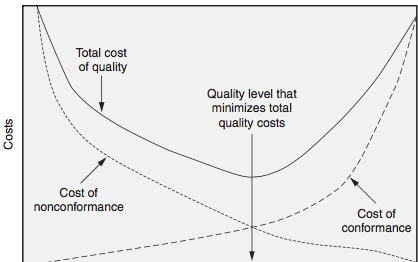
\includegraphics[width=90mm]{imagenes/CurvaCostesCalidadInicio.png}
\caption{Curva de Costes de Calidad antes de iniciar el desarrollo.}
\label{fig:CurvaCostesdeCalidadInicio}
\end{figure}

En la primera ronda de medidas de costes nadie debe ser increpado, debe servir a modo comparativo y para sacar el qué hacer y el cómo hacerlo. La meta es intentar llegar a la Fig \ref{fig:CurvaCostesdeCalidadFin}.

\begin{figure}[ht!]
	\centering
	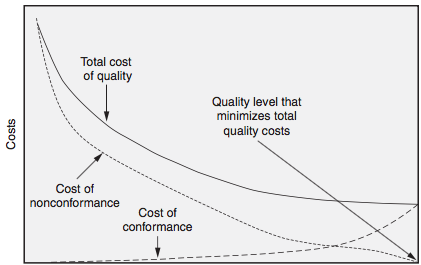
\includegraphics[width=90mm]{imagenes/CurvaCostesCalidadFin.png}
	\caption{Curva de Costes de Calidad al final del desarrollo.}
	\label{fig:CurvaCostesdeCalidadFin}
\end{figure}

Una técnica para desarrollar estrategias es la planificación \textit{hoshin}. Desarrollar 4 visiones de lo que debería ser la compañía en 5 años.

\begin{equation}
Expected \, Profit  = \sum Profit \, \mathrm{x} \, Probability
\end{equation}

Cuando un sistema trabaja por debajo de su nivel óptimo es \textit{suboptimization}.

\subsection{Conductores de la organización y métrica}
Factores clave: hay que sacar datos e información de clientes, productos, servicios, operaciones, mercado, competitividad, proveedores, sindicatos, costes, gobiernos y cumplimiento del rendimiento mediante indicadores.

\textbf{Voice of the Customer (VoC)}: donde factor clave es el cliente y el conocimiento del mercado: las relaciones con clientes y la habilidad de determinar cómo adquirir un nuevo cliente, satisfacerlo, conseguir su lealtad para retenerlo y expandir el mercado. \textit{VoC} es el proceso para capturar información relacionada con los clientes. La intención es anticiparse a los requerimientos de cliente, necesidades y deseos. La meta es conseguir la lealtad para construir relaciones entre-con clientes. VoC puede incluir reunir e integrar datos de encuestas, datos de la web, datos de garantías, registros de quejas y toda aquella información que afecta a la compra y a las decisiones que toma un cliente.

\textbf{Balanced Scorecard (BS)} (tarjetas de puntuación equilibradas): Sistema que permite a las organizaciones centrarse en su visión y estrategia, y afinar con las acciones a desarrollar. Provee \textit{feedback} en procesos internos y externos. Una vez completamente integrado, el \textit{BS} convierte el plan estratégico en el centro nervioso de la empresa.

\begin{figure}[ht!]
	\centering
	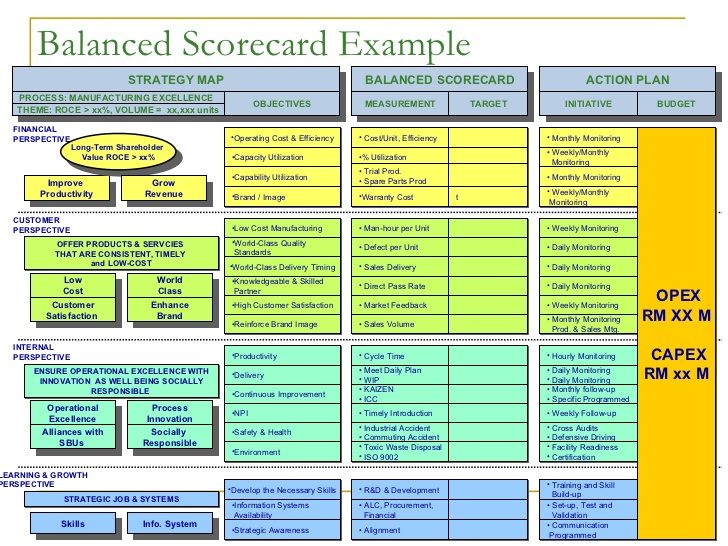
\includegraphics[width=140mm]{imagenes/BS.jpg}
	\caption{Ejemplo de Balanced Scorecard.}
	\label{fig:Balanced ScoreCard}
\end{figure}

\textbf{Scoreboard/Dashboard}: representación visual que da una visión rápida de la compañía a tiempo real. Es crítico para ayudar al empleado a predecir ventas, cash flow, beneficio y da claridad a la actuación y dirección de la compañía. Debe ser una herramienta crítica de toma de decisiones usada en las operaciones del día a día. Tres pasos para construir un efectivo \textit{Dashboard}: \begin{enumerate} \item Conocer los promedios y el benchmark de la industria. \item Conocer su posición y trayectoria sobre estos promedios y el benchmarking. \item Desarrollar cada llamada al \textit{BS} en un conjunto comprensivo de la compañía, no solo las partes implicadas. \end{enumerate}

\textbf{Key Performance/Process Indicator (KPI)} (indicador clave de rendimiento): Medida cuantificable que acordada de ante mano, refleja el éxito de los factores críticos. Hay que saber elegir que medidas necesitas para controlar o perseguir en tus proyectos. 

\section{Principios Lean en la organización}

\textbf{¿Qué es Lean?}: añadir o mantener valor en lo que se hace, reducir \textit{waste} y el proceso de crear valor sin \textit{waste}. Ceoncepto: Añadir valor sin reducir nada más. Toyota Production System es el origen y la clave del Lean. 

\begin{figure}[ht!]
	\centering
	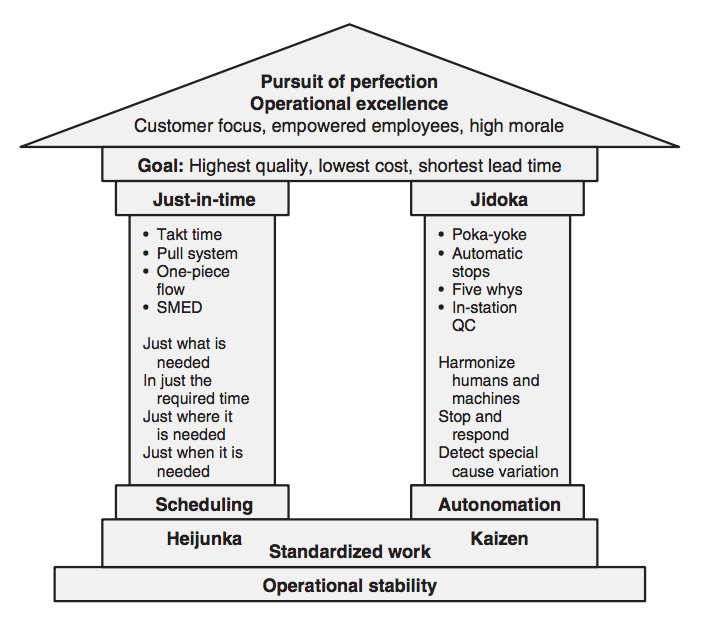
\includegraphics[width=120mm]{imagenes/TPSHouse.png}
	\caption{TPS House}
	\label{fig:TPS House}
\end{figure}

\subsection{Value}

El concepto que mas preocupa a los negocios en los años recientes es el \textit{valor}. La percepción de la utilidad y necesidad de un producto o servicio. 

La gente coge coches japoneses por calidad, confianza y eficiencia. La gente coge coches alemanes por otros valores, el orgullo de marca por ejemplo. Los coches americanos son comparables con ambos, pero ellos creen en la lealtad del cliente. 

Un paso tiene valor añadido dentro de un proceso si: \begin{itemize} \item el cliente reconoce el valor del producto/servicio. \item puede transformar el producto. \item el producto está bien hecho a la primera. \end{itemize}

\textit{Non-value-added} o \textit{rework}, son actividades por las que el cliente no está dispuesto a pagar. El cliente está dispuesto a pagar por la impresión de un documento pero no por las correcciones del proveedor. Hay que cuestionarlo todo para identificar las actividades \textit{non-value-added}. Siempre hay zonas grises entre valor añadido y no valor añadido. Esto ocurre con inspección y testeo. El cliente no quiere problemas, por lo que inspección es valor añadido, pero la solución es mejorar el proceso hasta el punto de que no tenga que ser inspeccionado. Por otro lado, el sello de la IFS da categoría, así que hacer lo que el sello pida es lo propio, ya que tenerlo da un valor añadido.

Los 14 principios del \textbf{Camino Toyota}: \begin{enumerate} \item Decisiones de gestión en una filosofía de largo plazo. \item Proceso continuo que lleve los problemas a la superficie. \item Sistema \textit{Pull} para evitar sobreproducción \item Nivelación de carga de trabajo \item Construir cultura de parar a arreglar problemas para tener calidad desde el primer momento \item Estandarizar tareas y procesos \item Controles visuales \item Utilizar tecnología fiable y probada \item Crecer líderes que entienden el trabajo a fondo, vivan la filosofía y enseñen a otros \item Desarrolla gente y equipos que sigan la filosofía de la compañía \item Respeta la red de compañeros y proveedores retándolos y ayudándolos a mejorar \item Ve y mira por ti mismo para entender la situación \item Toma decisiones en consenso y teniendo en cuenta todas las opiniones \item Empieza una organización que aprenda la mejora continua. \end{enumerate}

\subsection{Herramientas Top Lean}

\textbf{5S (o 6S, o 7S)}. Método de organización del lugar de trabajo para mejorar la eficiencia. El orden: \textit{Sort}: Lo que no hace falta o rara vez hace falta, fuera. Muchas cosas da lugar a desorden y desorden da lugar a pérdida de tiempo. \textit{Set in order}: Colocación de las cosas necesarias en el sitio necesario: instrucciones, herramientas, gafas de seguridad. \textit{Shine}: la limpieza es importante. Una vez resuelto (si es un ejercicio intelectual) hay que dejarlo bien organizado y limpio para que se entienda, esa es la filosofía de la limpieza. \textit{Standarize}: desarrollar checklist, starndarts e instrucciones de trabajo para tener un orden. \textit{Sustain}: mantener las otras 4 S. Las 5S mejoran la productividad y la eficiencia, reduce los accidentes. La gestión debe dar poder a los empleados para que ellos puedan tener propiedad sobre sus áreas de trabajo. Las otras dos son: \textit{Safey}-seguridad y \textit{Oversight}-asegurar a la primera.

\begin{figure}[ht!]
	\centering
	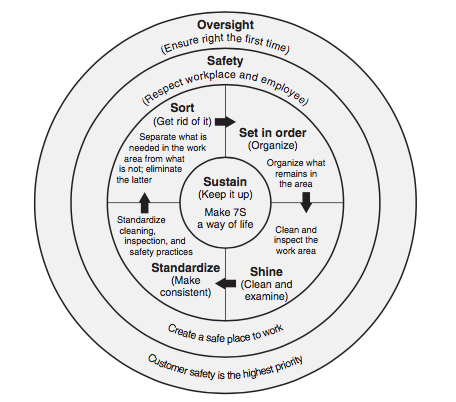
\includegraphics[width=90mm]{imagenes/7S.png}
	\caption{7S adaptation}
	\label{fig:Las7S}
\end{figure}


\textbf{Andon}. Sistema de \textit{feedback} visual (semáforo) para advertir del nivel de calidad de producto.

\textbf{A3}. Un formato A3 que contenga: Antecedentes, Situación Actual, Análisis de Causas, Objetivos de Mejora, Acciones de mejora, Plan de acción, Seguimiento de los resultados. No todos los problemas necesitan un A3, solo los complejos y no-evidentes.

\textbf{Gemba}. Ir a planta, allí es donde ocurren las cosas. Gestión mientras caminas.

\textbf{Heijunka}. Calendario productivo orientado en hacerlo en pequeños bloques de secuencias, en el mismo proceso. Para reducir tiempos muertos y tener bajos niveles de inventario.

\textbf{Hoshin Kanri}. Quality Function Deployment. Consiste en alinear las metas de la compañía (strategy) con los planes a medio plazo (tactics) y las operaciones de trabajo (actions). 

\textbf{Jidoka (Autonomation)}. Por qué hacerlo a mano si una máquina lo puede hacer mejor. Sobre todo si son cosas tediosas. 

\textbf{Kaizen Continuous Improvement vs Kaizen Events}. Mejora continua. \textit{Kaikaku} es un evento Kaizen. Resultados rápidos. Apoyo de la gestión para cada iniciativa. Si los empleados no pueden mejorar el proceso entre 3 - 5 días, la organización necesita reajustar la cultura.

\textbf{Kanban (Pull System)}. El sistema es mejor controlado cuando material e información fluye hacia dentro y fuera de los procesos de manera suave y racional. Ocurre que muchas veces llega antes de tiempo, informacion confusa... Un sistema Kanban da la información necesaria en el momento oportuno. Funciona usando unas \textit{visual cards}.

\textbf{Overall Equipment Effectiveness (OEE)}. El concepto de medir la efectividad de una operación: \textit{availability, performance and quality}. A * P * Q. 

\textbf{Single Minute Exchange of Die (SMED)}. Rápido y efectivo camino para convertir un proceso operativo en un producto hacia el siguiente. Los grandes cambios son la clave para reducir lotes de producción.

\textbf{Standar Work}: 9001, con su mapa de procesos, procedimientos, ...

\textbf{Takt Time} del alemán \textit{taktzeit}. La batuta de una orquesta. Metas, velocidad, tiempos. Ajustar producción con demanda.

\textbf{Theory of Constraints}. Metodología de problema-solución que busca el enlace más debil de la cadena. Normalmente es el mas lento. Identificar, Explotar (mejorar), Subordinar (el resto a este), Elevar (revisiones, inversiones, mejora de la debilidad) y Repetir.

\subsection{Muda}

El \textit{waste} (muda) viene de varias fuentes:

\textbf{Overproduction}. Hacer mas de lo que necesita el siguiente proceso. Principal síntoma \textit{Work In Process WIP}.

\textbf{Excess motion}. Workplace layout. Problemas de ergonomía, tiempo gastado buscando o moviendo provisiones o equipo.

\textbf{Waiting}. Esperas, setups largos, gente que no aparece o se demora...

\textbf{Inventory}. ¿Tienes inventario? El control sobre él, es un gasto. Equilibrio entre el control de stock vs ciclo económico, el retorno de la inversión. Estudio de equilibrado de costes.

\textbf{Excess Movement of Material/Transportation}. Los movimientos de handling y storing matan. Un plant layout bien puesto sirve para evitar esto. Departamentos orientados a la función propia necesitan de muchos movimientos.

\textbf{Defect Correction}. Corregir defectos. Actividad non-value added. Tipicas causas: mal  mantenimiento, mal sistema de calidad, malas instrucciones de trabajo y/o mal diseño. 

\textbf{Excess Processing/Overprocessing}. Difíciles de reconocer. Demasiados procesos. 

\subsubsection{Otros}

\textbf{Falta de creatividad}. Empleados tienen que tener ideas para mejorar los procesos.

\textbf{Perfección}. Evitar la perfección exacta. 

\subsection{Value Stream Mapping} 

\textit{Value Stream} es una serie de actividades que hace una empresa: pedir, diseñar, producir, entregar productos/servicios. Un value stream empieza por los proveedores de los proveedores y acaba con los clientes de los clientes. Componentes: \begin{enumerate} \item \textit{Flow materials} desde proveedor hasta entrega a cliente (los pedidos entran semanalmente en camión, los materiales se mueven hasta la zona de producción y al almacén de producto terminado, producto terminado se entrega a cliente), \item \textit{Transformation of raw materials} (pasos de producción rollo cortar, moldear, forjar...), \item El flujo de información requerido para ayudar al flujo de material y a la transformación (órdenes de compra a proveedores, órdenes internas de trabajo, shipping notice...). \end{enumerate}

Value Stream Map usa gráficos con iconos simples para ilustrar el movimiento del material, inventario, work-in-progress, operadores... Un Value Stream Analysis es el que descubre \textit{wastes} ocultos en la organización. Aplicar \textit{Lean Thinking} para dividir un camino-\textit-{path} en diferentes pasos: \begin{enumerate} \item Producir un \textit{value stream map (value chain diagram)}. \item Analizar las notas de inventario pensando en reducirlo o eliminarlo (inventario = coste del espacio, perdida de calidad, diferentes versiones (v2 v3 v4...), el dinero se puede invertir en otras cosas), \item Analizar los non-value steps para eliminarlos, \item Determinar como es conducido el flujo (p.e.: en función de pedidos del cliente), 5. Extender el Value Stream Map hasta los proveedores (compatibilidad entre sistemas-codigos de barras). \end{enumerate}

\begin{figure}[ht!]
	\centering
	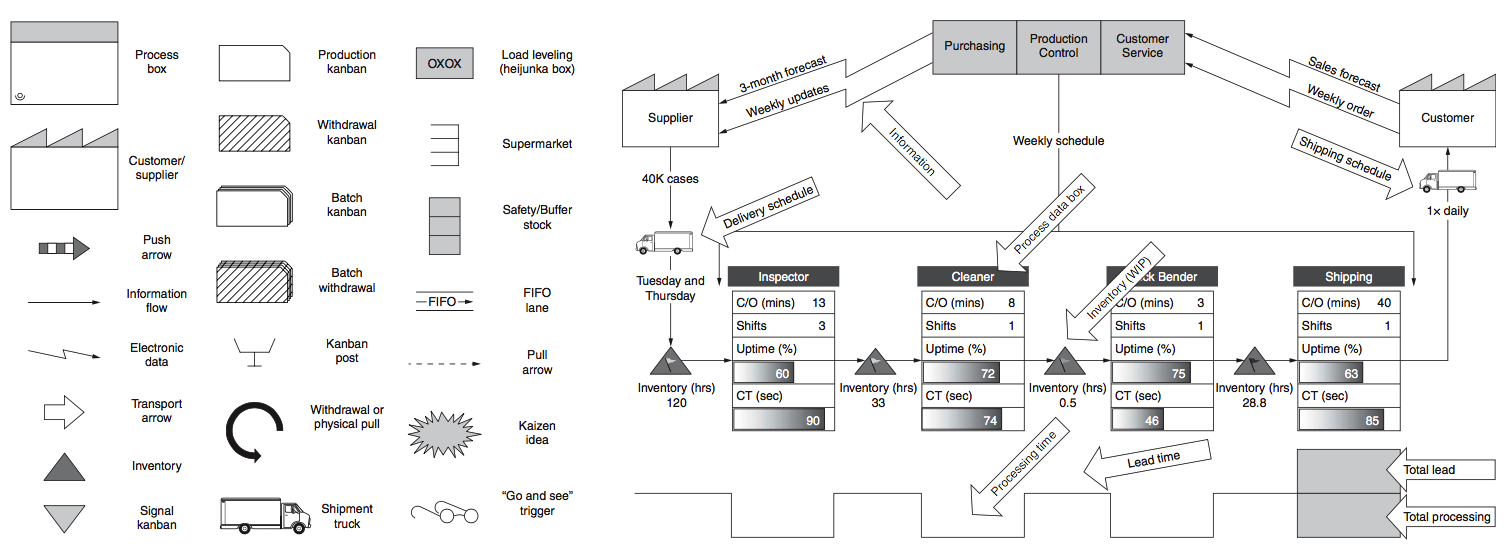
\includegraphics[width=170mm]{imagenes/ValueStreamMapping.png}
	\caption{Value Stream Mapping}
	\label{fig:ValueStreamMapping}
\end{figure}

\section{Diseño para metodologías Six Sigma (DFSS)}

DFSS se apoya proceso estratégico de negocio/ingeniería y en procesos capaces de reducir y gestionar variaciones: con DMADV (define, measure, analyze, design, verify) y con IDOV (identify, design, optimice, verify). Hay batiburrillo de sigmas DFSS, DCOV, ICOV, DMEDI, IDDOV, GD. Se use el que se use, pero hay que recordar: robustez del sistema usado, no abrir mil proyectos, uno para cada síntoma, evitar perder el tiempo alimentando el sistema de datos y ratings, alcance vago o pequeño. Lo que no puedes controlar se llama \textit{noise}-ruido. \textit{noise strategy} para mejorar el proceso.

Usamos DFSS para aumentar la satisfacción de cliente, reducir variaciones, tener un diseño robusto, bajar costes de garantía, mejorar durabilidad, incrementar facturación-ganancias y producción (ésta última a través de reducir el número de \textit{downtimes} debidos a defectos).

\subsection{IDOV} \textit{Identify} - \textit{Design} - \textit{Optimize} - \textit{Verify} similar al MAIC del Six Sigma (\textit{measure, analyze, improve, control}).

\textit{Identify Phase}: identificar requisitos de producto y cliente, establecer caso de negocio, identificar aspectos técnicos, variables critical to quality (CTQ), límites de especificaciones, roles y responsabilidades e hitos.

\textit{Design Phase}: Formular el concepto, identificar posibles riesgos usando FMEA \textit{(failure mode and effects analysis)}, para cada detalle técnico, identificar parámetros diseño, usar DOE \textit{(design of experiments)} y otras herramientas de análisis para determinar CTQs y su influencia en los requisitos técnicos.

\textit{Optimize Phase}: Evaluar las posibilidades del proceso y llegar a conocer bien los límites CTQ. Optimizar el diseño minimizando los CTQs, prueba-error, estadísticas y tolerancias.

\textit{Validate Phase}: Prototipado, evaluar actuación, fallos, confianza y riesgo, reiteración en el diseño y revisión final de producto.

\subsection{DMADV} Para cuando el producto no existe y ha de ser desarrollado, o sí que existe pero no se conocen las necesidades del negocio o del cliente. 

\textit{Define}: Targeting prioridades.

\textit{Measure}: Combinación de análisis técnico y competitivo del producto. 

\textit{Analyze}: Aproximaciones de estadística e investigación, para establecer prioridades y confianza.

\textit{Design}: \newline Design for/to Cost: búsqueda de alternativas en procesos, materiales, métodos... \newline Design for Manofacturing/productibility/assembly: pequeños cambios que hacen que sea mucho mas barato fabricarlo. \newline Design for test: donde testing es crítico, lo mejor es hacer test tempranos en el ciclo de producción. \newline Design for maintability: aplicable si se necesitan muchos \textit{downtimes} y reparaciones. \newline Design for Robustness: test en todos los ciclos de vida, y partes, ensamblajes y subensamblajes. \newline Design for usability: Validación! puede ser medido y mejorado. Extended for functionality: otras características desde el punto de vista del diseño. \newline Design for efficiency: consumo mínimo de recursos. \newline Design for Performance: la mejora de los microchips es un ejemplo. \newline Design for security: preserva la integridad del producto. Design for scalability.

\textit{Verify}: Es necesario asegurar los resultados del diseño de los objetivos. 

\subsection{FMEA} Se utiliza FMEA para evaluar el proceso o el producto y determinar \textbf{qué} causa el fallo y los \textbf{efectos} que pueden tener. 
Identifica y usa escala, calcula el Risk Priority Number (RPN) y analiza los resultados.

La esencia del \textit{failure mode and effects analysis} es el estudio del riesgo. Riesgo es lo incierto de un evento. Riesgo es la posible influencia buena o mala de un producto en un entorno. El riesgo se puede definir como impact (severity), probability (ocurrence) y event (detection). Segun Risk Road Map ISO 31000:2009 gestión del Plan risk / herramientas del risk identification / analizar y evaluar riesgos / plan risk response / monitor y control del risk.

\begin{figure}[ht!]
	\centering
	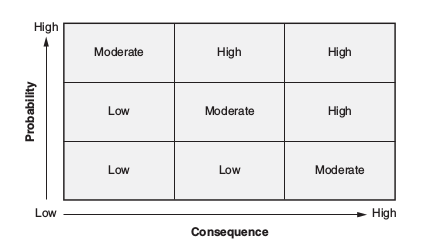
\includegraphics[width=90mm]{imagenes/RiskMatrix.png}
	\caption{Risk Matrix en FMEA PRN.}
	\label{fig:kMatrix}
\end{figure}

FMEA es una herramienta front-end. Un producto/proceso de éxito requiere anticiparse a los problemas y para ello hace falta tener jerarquizados cuales atacar antes, y/o como atacarlos. \textbf{Mirar Effective FMEAS}. El documento de gestión FMEA se tiene que ir controlando por versiones, incluyendo y quitando cosas, ya que es un documento vivo. Los beneficios del FMEA: evaluación a todos los clientes (internos y externos), ayuda en la evaluación de requerimientos y alternativas, ayuda a centrarse en dónde pueden aparecer los problemas críticos y como paliarlos/evitarlos/controlarlos, ayuda en el desarrollo de una lista de actuaciones priorizada, ayuda a evaluar el propósito del proceso...

\begin{figure}[ht!]
	\centering
	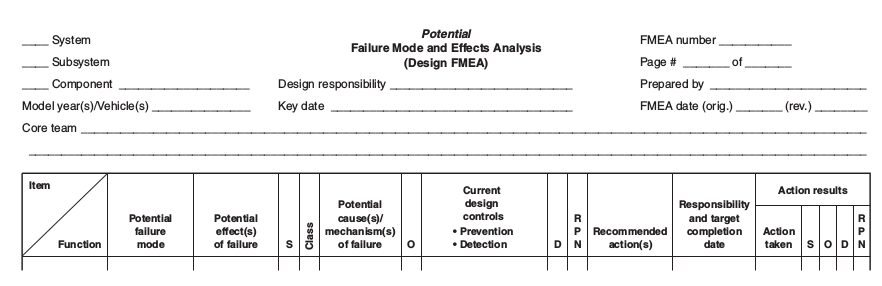
\includegraphics[width=170mm]{imagenes/PlantillaFMEA.png}
	\caption{Cabecera de una plantilla FMEA}
	\label{fig:PlantillaFMEA}
\end{figure}

\begin{figure}[ht!]
	\centering
	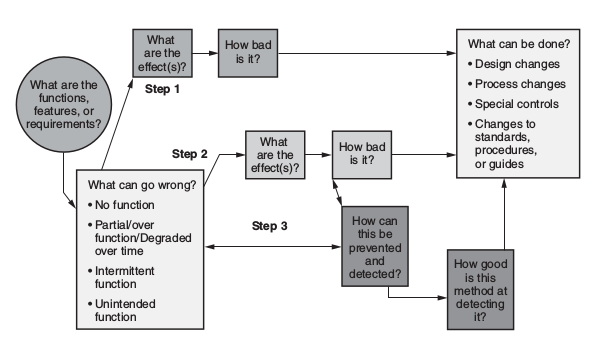
\includegraphics[width=90mm]{imagenes/FMEAFlowchart.png}
	\caption{Diagrama de flujo de FMEA}
	\label{fig:FMAFlowchart}
\end{figure}

Pasos del FMEA: \begin{enumerate} \item Lista los pasos claves de un proceso \item \textit{Brainstorm} de porque puede fallar cada paso \item Lista de efectos de los fallos \item Ranking de severidad para los efectos \item Causa y frecuencia de los fallos \item Controles para la detección \item Cálculo RPN \item Ordenar por críticos los RPN. \item Desarrollar plan de acción, asignando persona-responsabilidad \item Re-Calcular el RPN una vez implantado. \end{enumerate}

\subsubsection{Do's} 1. Da formacion de FMEA antes de asignar equipos 2. Enfoque de equipo 3. Pregunta a expertos si es necesario 4. Habla con el cliente de como va a utilizar el producto 5. brainstorm de los posibles fallos. 6. Si dos riesgos tienen la misma RPN, se queda encima el que tenga mas severidad. 7. completa la acción y reasigna la severidad. 8. Actualiza el FMEA con los nuevos riesgos aprendidos.

\subsubsection{Don'ts} 1. No copies el S-O-D de una industria a otra. 2. Intenta no usar una escala de 1-10, mejor de 1-5. 3. No hagas escalas especializadas sino es completamente necesario. 4. No manipules los datos.

\begin{figure}[ht!]
	\centering
	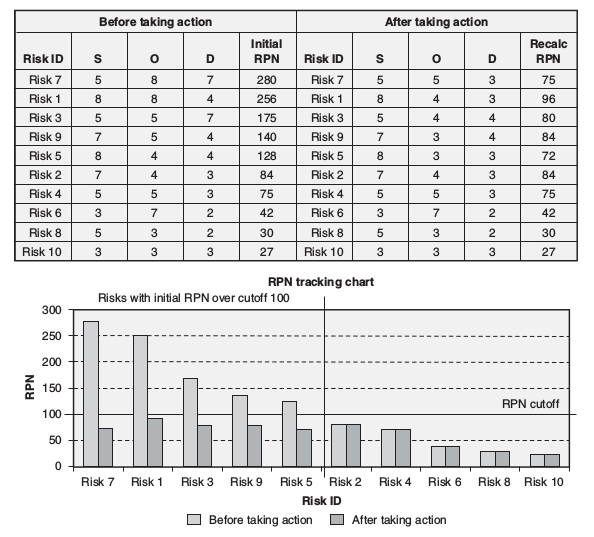
\includegraphics[width=140mm]{imagenes/FMEAPrePos.png}
	\caption{Report final de un FMEA}
	\label{fig:FMEAPrePos}
\end{figure}
\pagebreak[4]
\part{Definición}

Preguntas críticas de la fase de definición: ¿dónde estamos? ¿cuál es el problema? ¿dónde queremos estar? ¿cómo vamos a llegar allí? ¿cómo sabremos que hemos llegado a ese punto? \newline Antes de empezar, comprobar que la gestión y la economía del proyecto están alineadas. Mas tiempo frente a una buena planificación, mayor será el éxito. 

\section{Identificación del proyecto}
\subsection{Project Selection}

Describir el proceso de selección de proyecto y que factores deben ser incluidos para considerar si usar DMAIC u otro tipo de proceso problema-solución. Lo suyo es que haya un departamento o comité para decidir qué proyectos se pueden llevar a cabo y cuales no, ya que todas las ideas a la vez son imposibles. Cada propuesta debe tener medidas sobre el problema que plantean resolver y el impacto de éstas sobre la organización. Managers suelen coger la solución que ahorre más dinero a la compañía. \newline
Proyectos que tengan que ver con el análisis de datos, para el equipo de Six Sigma. Los que tengan que ver con mejora de procesos, con el equipo de Lean Manufacturing.

\subsection{Process Elements}

Definir y describir los componentes del proceso	y límites (boundaries). Reconocer como los procesos cruzan varias areas funcionales y los retos que resultan de los esfuerzos de mejora de procesos. Los procesos se pueden subdividir en subprocesos.
Por ejemplo, el proceso de \textit{payroll} tiene subprocesos: reunir la información del reloj de fichar, aplicar deducciones, ...

Para definir bien un proceso hay que marcar donde empieza y donde acaba: los límites (\textit{boundaries}). Los procesos transversales pueden tener subprocesos límite, definidos por la estructura del negocio, geografía...

\subsection{Benchmarking}

Entender que hay varios tipos de benchmarking, incluyendo la competitividad, la colaboración y las buenas prácticas.
Pueden ser comparativas internas, contra otros procesos internos o externas. Las fuentes de información del Benchmarking vienen de publicaciones, reuniones profesionales, investigaciones universitarias, \textit{feedback} de clientes, visitas, análisis de productos de competidores...

Operaciones de Benchmarking: analizar la operativa, conocer los líderes del mercado, incorporar lo mejor de lo mejor, ganar superioridad. 

Internal benchmarking: fácil acceso a otros dptos. sin embargo, el límite de mejora está reducido al estilo de la compañía.

Competitive benchmarking: fuerza a la compañía a tener una perspectiva externa. Sin embargo, fijarse en las prácticas de las industrias puede limitar el alcance de altos niveles de actuación.

Funcional benchmarking: comparas funciones similares, normalmente se busca fuera de la empresa y permite conseguir más partners de benchmarking.

Collaborative benchmarking: cooperación entre varias organizaciones para lograr resultados de benchmarking. Esta práctica permite el acceso a benchmarking partners  mas específicos.  

\subsection{Inputs y outputs de procesos}

Identificar las variables del \textit{input} y las del \textit{output} y evaluar sus relaciones usando \textit{Supplier, Inputs, Process, Output, Customer} (modelo \textit{SIPOC}).

Es clave definir los límites del proyecto, o comienza el fracaso de la mejora de procesos.

Dividir los procesos por functional areas (dptos) y organizations (suppliers, intercompany, teammate company, ...), esto se puede identificar con diagrama SIPOC y con un flowchart estilo swim-lane y un mapa de procesos podemos reconocer las interacciones entre ellos. Retos que te encuentras cuando defines esto: quien es el dueño del proceso, quienes comparten información, medidas (¿en qué mides? camiones/horas, euros/día), conocimiento del proceso (supply chain no sabe como funciona manufacturing).

Si los retos tienen riesgos potenciales asociados, hay que asociar actividades para minimizarlos.

\subsubsection{Systems Thinking}

La identificación y consideración de todos los diferentes elementos individuales que interaccionan con un propósito común a hacia una gran función se considera \textit{System Thinking}. \textit{ST} es sobre usar herramientas y métodos disponibles para saber que se está haciendo en una operación específica y cómo esa actividad afecta tareas y productos posteriores. También, el cómo priorizar tareas. \newline \textit{ST} sirve para entender mejor los procesos y como influyen los parámetros. \newline Ejemplo: proveedor envía X producto con algo mas de humedad de la cuenta, \textit{ST} especificaría como hay que modificar el proceso para que se ajuste. 

\subsection{Dueños y Stakeholders}

Identifica los dueños de los procesos y los diferentes grupos de interés (stakeholders) en un proyecto.
Los dueños de los procesos son los que tienen la responsabilidad de ejecutar e implementar procesos específicos. Los mejores métodos para mejorar los procesos usan equipos de dueños y de todos los stakeholders ya que éstos últimos tienen mejor conocimiento sobre el proceso, sobre las ideas para mejorar, se preocupan por las consecuencias del cambio en un proceso. Por lo tanto stakeholders en un proceso son: operadores, managers, clientes, proveedores, ...

\section{Voice of the Customer (VOC)}

\subsection{Identificar al customer}
\textit{Customers} puede haber de dos tipos: internos, que trabajan en el proceso, externos. Pasa identificar customers internos los mejores métodos a utilizar: brainstorming, SIPOC, análisis de márketing, perseguir un producto por todos los pasos hasta la entrega.

Al igual, se pueden dividir los \textit{customers} por grupos: Internos/Externos, por edad, por localización, clima, lengua, por industria.

\subsection{Datos del customer}

Hace falta conseguir datos: encuestas, observar grupos, entrevistas, ... Identificar los elementos clave para hacer efectivas estas herramientas. Revisar colecciones de datos para eliminar indeterminaciones.
¿Cómo saber lo que el cliente quiere? preguntándole. El cliente es experto en lo que hace, sabrá lo que necesita. 

El foco para un Green Belt es, internamente, hablar con la gente para saber qué hacen y cómo podríamos hacer que fuera más fácil hacerlo: lo que quiere, requisitos y expectativas. 

Para capturar datos del \textit{customer} podemos utilizar: VoC, surveys, QFD (Quality function deployment), entrevistas, ...

Lo suyo es seleccionar aleatoriamente un gran grupo de clientes y aplicar un método de manera estadísticamente válido ya que la información debe ser objetiva, con precisión y consistencia, evitando la ambigüedad. 

\subsection{Requisitos del cliente}

Usamos QFD (\textit{Quality Functions Deployment}) para traducir los requisitos del cliente en características del producto y oportunidades de mejora. Una de las aplicaciones mas importantes de Six Sigma es diseñar y rediseñar procesos y productos, para conseguir el menor coste posible.

QFD (o \textit{House of Quality}) tiene de input VoC. La matriz QFD muestra el enlace entre VoC y los requisitos técnicos resultantes.

\begin{figure}[ht!]
	\centering
	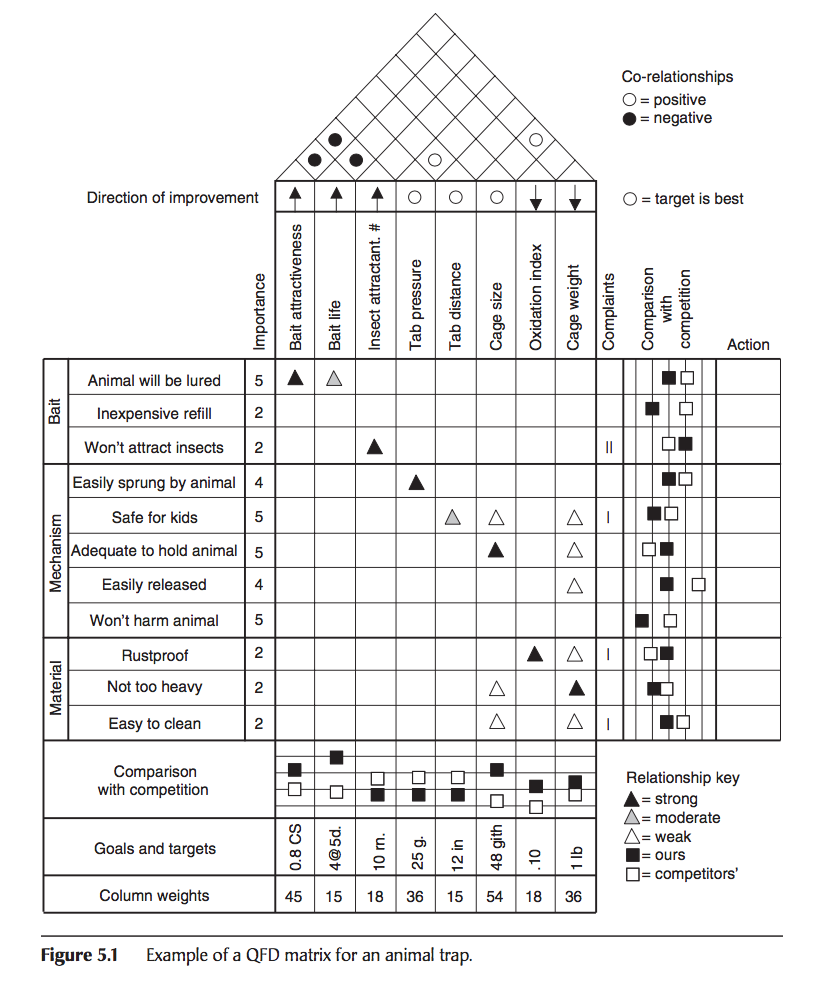
\includegraphics[width=150mm]{imagenes/ExampleQFD.png}
	\caption{Ejemplo de un QFD}
	\label{fig:ExampleQFD}
\end{figure}

QFD puede ser aplicado para mejorar calidad. En la matriz, los \textbf{What's}, se traducen por \textit{must have} o por \textit{expected to have}. QFD ayuda a conducir los procesos mediante la calidad hasta el cliente.

\section{Project Management Basics}

\subsection{Project Charter}

\begin{quote}
Describir y definir elementos de un Project Charter, desarrollar el problema que incluya datos base o el estado actual para ser mejorado y las metas del proyecto.
\end{quote}

Un \textit{charter} es un documento de declaración con el propósito del proyecto.
Permite tener a los equipos de desarrollo alineados con la dirección de la empresa y debe incluir: 

\begin{itemize}
	\item Problem statement. Qué necesita ser mejorado.
	\item Purpose. Establece metas y objetivos del proyecto.
	\item Benefits. Por qué irá mejor la empresa cuando se consiga el objetivo.
	\item Scope. Limitaciones: tiempo, presupuesto, recursos, ...
	\item Results. Define el criterio y métricas para el éxito del proyecto.
\end{itemize}

La \textit{Project Planning} nos acerca a la monitorización del cómo y cuándo un proyecto será llevado a cabo. Será necesario tener información de los procesos, comunicación, negociación de recursos, \textit{incremental planning} y planificación modular, asegurar que los hitos sean medibles y faciliten una gestión enredada correctamente.

\subsection{Project Scope}

Usando SIPOC, brainstorming, diagrama de Pareto, podemos definir y documentar el alcance del proyecto. Lo habitual es que el alcance está basado en el \textit{Problem Statement}.

\subsection{Project Metrics}

Una planificación de proyecto sin la actuación de medición es poco menos que una actuación absurda. Las mediciones clave (\textit{key metrics}) enlazan directamente con las metas, habitualmente como: \textit{Percentage of work accomplished on time}, \textit{Percentage of work accomplished on budget}, \textit{disponibilidad de recursos}...

KPI (Key process indicators) es un valor medible que demuestra la efectividad de una compañía consiguiendo sus objetivos claves de negocio.

\subsection{Project Planning Tools}

Las herramientas para planificar proyectos más habituales son: Gannt, CPM (Critical Path Method) y PERT. Difieren según el tamaño y alcance del proyecto. La documentación se mantiene viva durante el desarrollo de todo el proyecto.

\subsection{Project Documentation}

Metas y objetivos. Sponsors y accionistas. Planificación y calendario. Hitos. Presupuesto. Límites. Roles y responsabilidades. Métricas para evaluar el proyecto.

Además del \textit{Project Charter} y el \textit{Project Management Plan} planes adicionales pueden ser utilizados para cada actividad.

\subsection{Project Risk Analysis}

El análisis de riesgo de un proyecto se incluye durante la fase de planificación. Identificar riesgos, asociar impacto y posibles planes para minimizar el riesgo. El análisis de riesgo hay que revisarlo y actualizarlo utilizando SWOT (\textit{strengths-weaknesses-opportunities-threats}), RPN, FMEA, \textit{formula for expected profit}.
Un buen análisis de riesgos necesita que los grupos apropiados estén presentes.

Aspectos de riesgo a considerar incluyen el impacto potencial en: conocer las metas establecidas, el calendario planificado, fuentes identificadas, seguridad, productividad, servicio, confiabilidad, conocer los requerimientos y expectativas del cliente.

\begin{figure}[ht!]
	\centering
	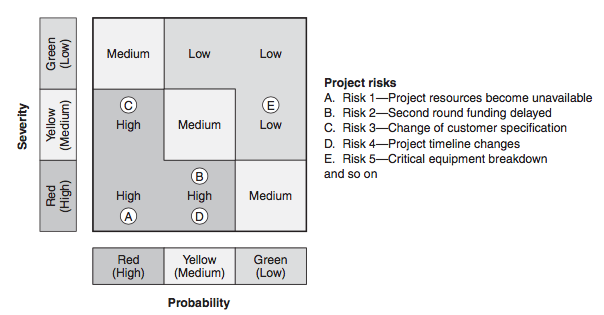
\includegraphics[width=120mm]{imagenes/RiskMatrix2.png}
	\caption{Matriz de riesgo}
	\label{fig:RiskMatrix2}
\end{figure}

A través de cosas que ya han pasado antes, riesgos, brainstorming se determinan los Project Risks. Después de identificarlos, minimizarlos y verificar las actuaciones que los pueden desencadenar son cosas que tienen que estar en el ciclo de vida del proyecto. 

\underline{Ejemplo de riesgo existente}: proveedor clave que no entrega a tiempo, la \textit{mitigation activity} es buscar un nuevo proveedor.
\underline{Otro ejemplo de riesgo existente}: un cajero automático, la \textit{mitigation activity} es: código de 6-10 cifras, bloqueo a los 3 intentos.

\subsection{Project Closure}

Revisar con los miembros y sponsors los objetivos logrados con el proyecto, asegurar que la documentación está completa y guardada apropiadamente. Identificar lecciones aprendidas e informar a otras partes de la organización sobre oportunidades de mejora.

\textit{Project Closure} no es negociación, es un paso final para conocer que metas y objetivos se cumplen, que la documentación está OK, y hacer una reunión para cerrar.

\textit{Project Charter} es una excelente herramienta para medir el progreso de un proyecto, con su alcance, metas, objetivos y una cronología.

\section{Management and Planning Tools}

\subsection{Activity Network Diagram}
Es como el PERT, muestra dependencias entre tareas y caminos (en serie o en paralelo). Al igual que PERT o \textit{Critical Path Analysis}, provee una visión global con nivel de detalle adecuado a la necesidad del proyecto.

\begin{figure}[ht!]
	\centering
	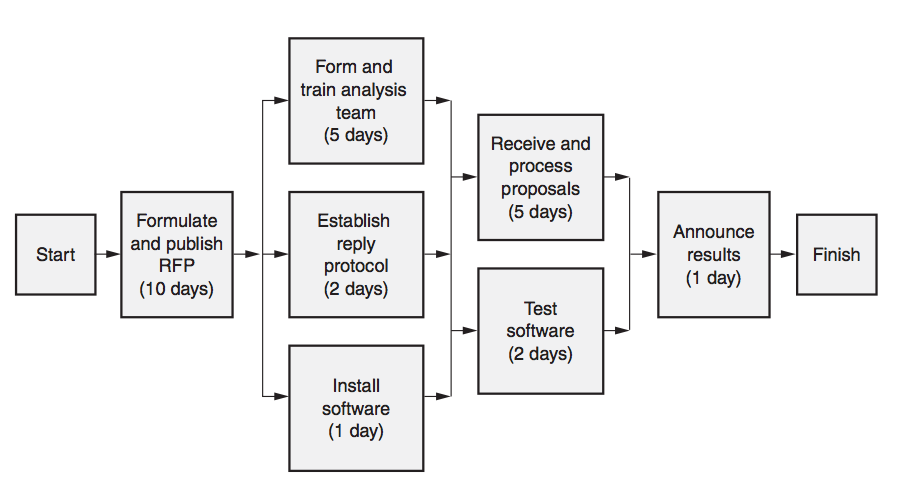
\includegraphics[width=120mm]{imagenes/AND.png}
	\caption{Activity Network Diagram}
	\label{fig:ANDDiagram}
\end{figure}

\subsection{Advanced Quality Planning} 

Se basa en la idea de que las planificaciones solidas previenen sorpresas y salvan recursos útiles de ser malgastados. AQP es un proceso donde primero buscamos los parámetros sobre lo que vamos a hacer. ¿tenemos suficiente material disponible? ¿tenemos la gente necesaria para hacer el trabajo?¿tenemos las herramientas necesarias para el trabajo? También se llama APQP. 
Es el primer paso del PDSA (Plan Do Study Act). Esto ayuda a que tengamos todos los \textit{inputs} para obtener el \textit{output} deseado. 

\subsection{Affinity Diagram}

Son usados para producir muchas respuestas a preguntas abiertas. Por ejemplo:¿qué maneras hay de reducir ciclo al proceso? Luego intentar asociar entre sí, en diferentes grandes grupos, dichas respuestas. Posteriormente, le damos nombre a la agrupación.

\begin{figure}[H]
	\centering
	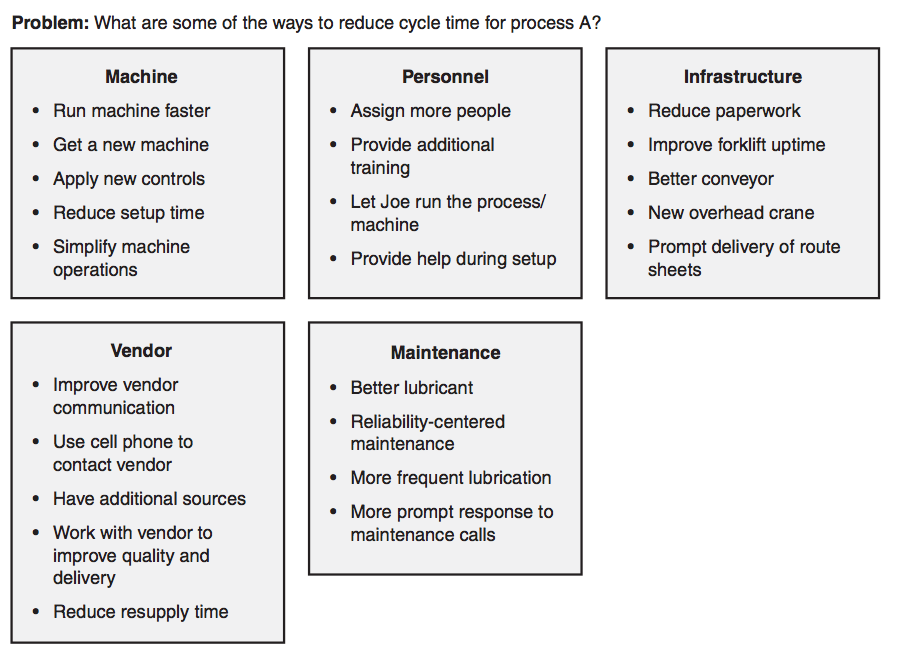
\includegraphics[width=120mm]{imagenes/AffinityDiagram.png}
	\caption{Affinity Diagram}
	\label{fig:AffinityDiagram}
\end{figure}

\subsection{Auditing}

Evaluación de procesos o proyectos contra planes y metas. Esta comprobación de auditoría de calidad es comúnmente establecida en organizaciones a través de sistemas de gestión de la calidad (AS9001, ISO 9001, ISO/TS 16949).

\textit{Audit planning}: preparación para el que va a ser auditado, un calendario de auditoria y una notificación de auditoría.

\textit{Audit performance}: evidencias, observaciones, entrevistas.

\textit{Audit report}: resumen con el alcance, actividades, resultados, \textit{findings} (acciones correctivas), oportunidades de mejora.

\textit{Audit closure}: actividades de seguimiento para asegurar que los planes en acción son implementados de manera efectiva.

Tipos: first-party, second-party, third-party, internal (mas usada en Six Sigma) y external.

Habitualmente están basadas en productos, sistemas, proveedores, cumplimiento normativo. Deja que te guie el auditor interno.

\begin{quote}
Be pleasant, you are not a cop. Be prepared. Be factual in what you observe, hiding things doesn't help to improve. Ask questions for clarity. Record your observations. 
\end{quote}

\subsection{Benchmarking}

Consiste en mirar un sistema y aplicar los conceptos de ese, sobre otro. La idea es hacer un win/win entre organizaciones. Pasos básicos: Flowchart del proceso actual. Identificar areas de mejora. Ideas-brainstorm. Investigar como otros hacen el proceso. Desarrollar planes de aplicación de ideas. Prueba piloto. Iniciar el nuevo proceso. Evaluar el nuevo proceso.

\subsection{FishBone Ishikawa}

Muestra factores envueltos en una situación. Crearlo a partir del 5W's (What, Why, When, Where, Who), 1H (How) y 6M's (Man, Machine, Methods, Materials, Measurement, Mother Nature, Money, Management).

\begin{figure}[H]
	\centering
	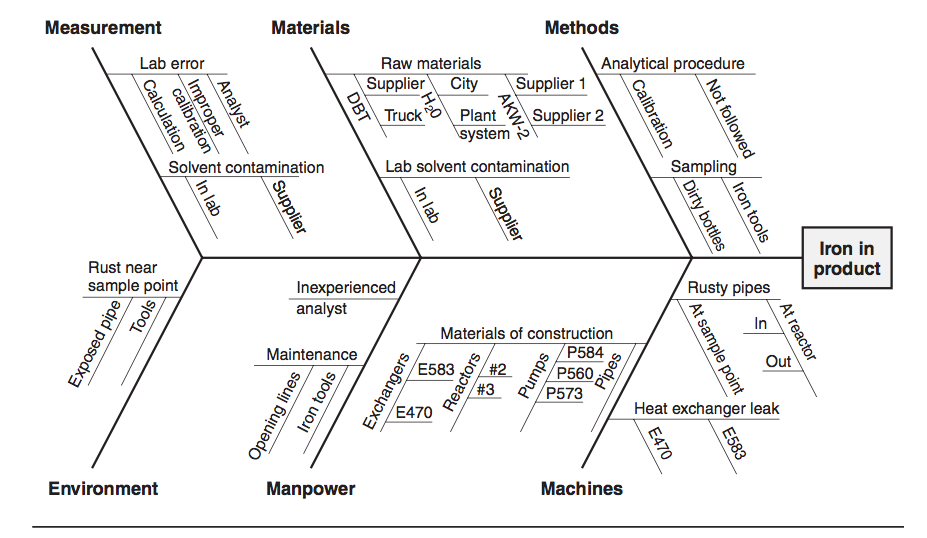
\includegraphics[width=120mm]{imagenes/FishBone.png}
	\caption{FishBone}
	\label{fig:FishBone}
\end{figure}

\subsection{Check Sheets}

Usadas para observar o revisar un proceso durante su ejecución. Pasos básicos en hacer un \textit{check sheet}: Identificar y agregar las causas o condiciones que han de ser recogidas. Decidir quien recoge la información, sobre cuantos periodos, y de que manera se recoge. Crear un \textit{check sheet} que ayuda a la mejora continua y puede fomentar cambios, solo por el hecho de utilizarla. La importancia de recoger datos es para asegurar consistencia y precisión de la información.

\begin{figure}[H]
	\centering
	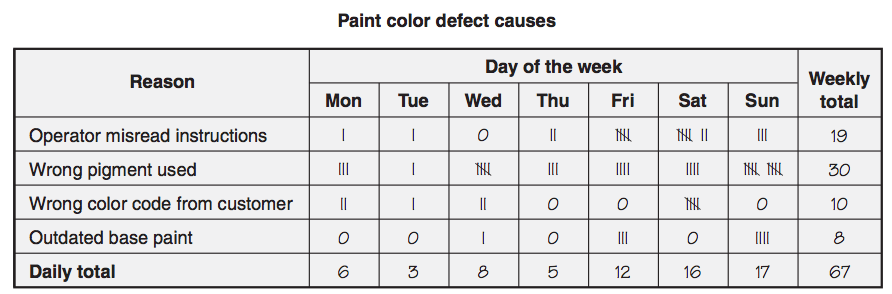
\includegraphics[width=120mm]{imagenes/CheckSheet.png}
	\caption{CheckSheet}
	\label{fig:CheckSheet}
\end{figure}

\subsection{Customer Feedback}

Encuestas, información vía emails, entrevistas dirigidas. Importante conseguir muestras representativas.

\subsection{Flowchart}

\begin{figure}[H]
	\centering
	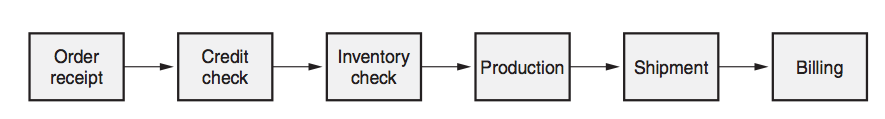
\includegraphics[width=120mm]{imagenes/Flowchart.png}
	\caption{Flowchart}
	\label{fig:Flowchart}
\end{figure}

Pasos: definir el proceso que va a ser diagramado. Decidir los límites del proceso. Averiguar cuales son las actividades que se dan lugar en él. Ordenar las actividades en secuencia. Crear un flujo de pasos con flechas. Que revise el \textit{flowchart} diferentes miembros de toda la organización.

\subsection{Focus Groups}

Identificar las metas de la sesión. Desarrollar productos actuales o prototipo. Determinar como las sesiones deben ser conducidas (\textit{brainstorming, survey, cause-and-effect, question-response}).

\begin{figure}[ht!]
	\centering
	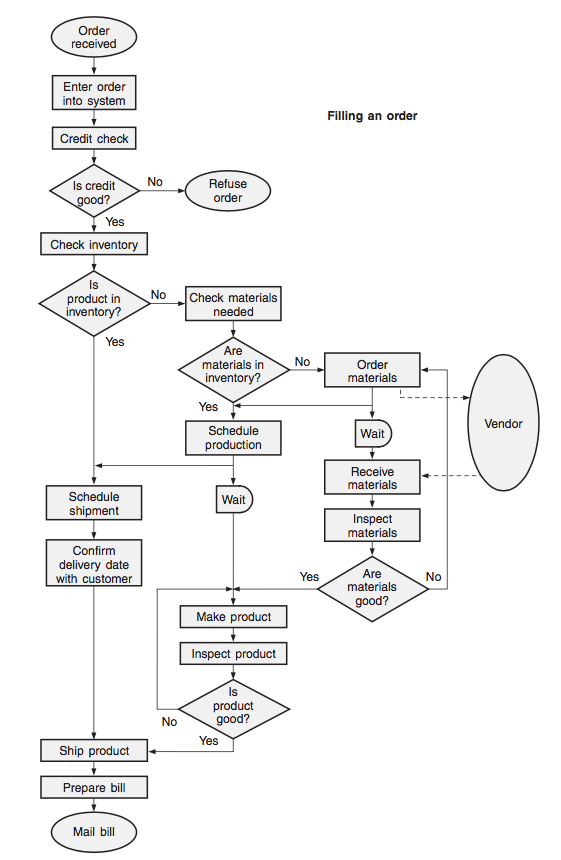
\includegraphics[width=120mm]{imagenes/DetailedFlowchart.png}
	\caption{Detailed Flowchart}
	\label{fig:DetailedFlowchart}
\end{figure}

\subsection{Force-Field Analysis}

Se pone un \textit{Future State} y se hacen dos columnas: \textit{Driving forces} y \textit{Restraining forces}. Cosas que suman/restan para conseguir el objetivo. A través del NTG (Nominal Group Technique) se hace un ranking con ellas. Y entonces se determina cómo proceder.

\subsection{Gantt Chart}

Gantt provee de un vistazo rápido las actividades planificadas y el calendario, permitiendo evaluar los recursos claves contra el plan, y también permite la evaluación de la actuación del proyecto frente al plan.

\subsection{Graphical, control and statistical tools}

\subsubsection{Variables Charts}

\begin{itemize}
	\item Averages and range chart.
	\item X and s chart.
	\item IX-MR, XmR, moving range chart.
	\item MA-MR chart.
	\item Target charts, deviation chart, nominal chart.
	\item CUSUM (cumulative sum chart)
	\item EWMA (weighted moving average chart)
	\item Hotelling T2
\end{itemize}

\subsubsection{Attributes Charts}

\begin{itemize}
	\item p-chart (proportion chart)
	\item np-chart
	\item c-chart (count chart)
	\item u-chart
	\item D-chart (total weighted deficiencies)
	\item U-chart 8average weighted deficientes per unit)
\end{itemize}

\subsubsection{Other Kinds of Data}

\begin{itemize}
	\item Short-run charts (Z-charts)
	\item Group charts (multiple characteristic charts)
	\item Paynter charts
\end{itemize}

\subsection{Interrelationship Diagram (DIGRAPH)}

Sirve para identificar relaciones causa-efecto. Normalmente se empieza listando media docena o una docena entera de preocupaciones, se ordenan y mediante flechas se dirige cual es mas importante que la anterior. Si no se dibuja flecha, es que no tiene importancia sobre otras.

Se compara cada una contra todas las que tiene relación. 

\begin{figure}[H]
	\centering
	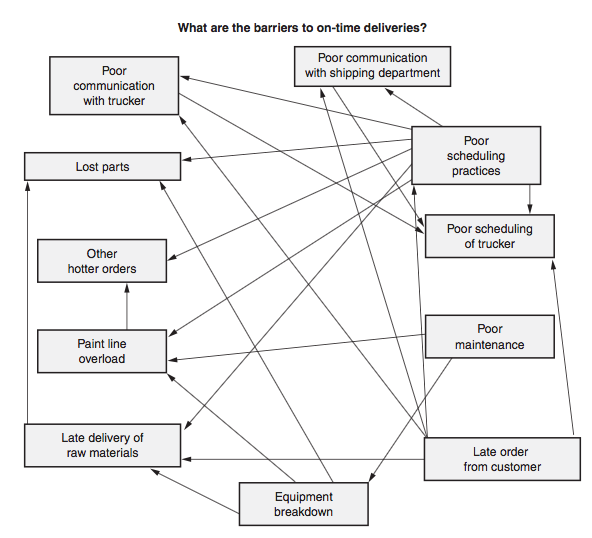
\includegraphics[width=120mm]{imagenes/interrelationshipdiagram.png}
	\caption{Interrelationship Diagram}
	\label{fig:interrelationshipdiagram}
\end{figure}

\subsection{Matrix Diagram}

Para descubrir relaciones entre dos grupos de items. 

\begin{figure}[ht!]
	\centering
	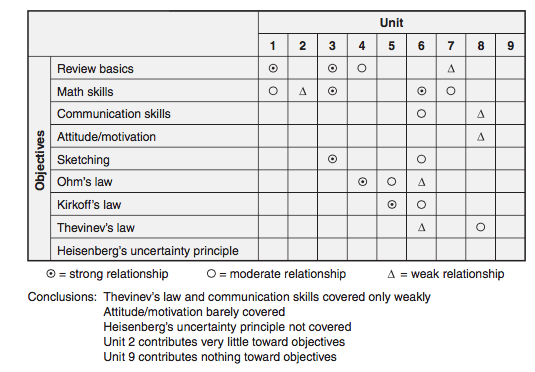
\includegraphics[width=120mm]{imagenes/MatrixDiagram.png}
	\caption{Matrix Diagram de un libro de texto}
	\label{fig:MatrixDiagram}
\end{figure}

\subsection{Nominal Group Technique}

Es un \textit{brainstorming} con una interacción limitada por grupos. Esto es para que no haya gente que diga mucho y otros no digan nada. El \textit{facilitator} explica las reglas, el \textit{team leader} presenta el tema y el equipo tienen como 10-15 minutos para sentarse, pensar y generar ideas.

No se permiten interacciones verbales, las ideas son recolectadas y puestas en un sitio donde todos puedan verlas. Los miembros deben leer las ideas en alto, una a una. A los miembros se les permite expandir las ideas, darles claridad, eliminar redundancia. El \textit{team leader} debe recoger las ideas y ponerlas en el \textit{board}, y mantener el anonimato de los contribuyentes.

\subsection{PDCA, PDSA y SDCA}

PDCA: Plan Do Check Act. PD\textit{S}A: Study. \textit{S}DCA: Standarize.

\subsection{Priorization Matrix}

Es una ayuda para decidir entre diferentes opciones. Para conseguir el criterio adecuado, se ponen los atributos de cada una de las opciones y se ponderan.

\begin{figure}[ht!]
	\centering
	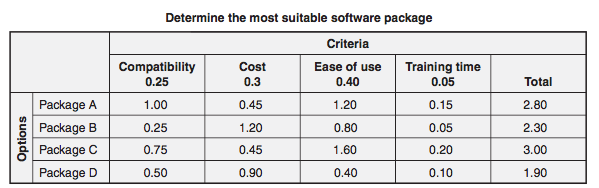
\includegraphics[width=120mm]{imagenes/Prioritizationmatrixexample.png}
	\caption{Prioritization matrix example}
	\label{fig:Prioritizationmatrixexample}
\end{figure}

\subsection{Problem Solving}

\textit{Eight Discipline Approach, 8D}. 

\begin{enumerate}
	\item Usa una \textit{team approach}. Organiza un pequeño grupo, que conozcan proceso y producto. Un campeón designado.
	\item Describe el problema. 5W2H, SIPOC, flowcharts.
	\item Empieza y comprueba las acciones. Define acciones, verifica la efectividad.
	\item Define y comprueba las raíces de la causa. 
	\item Comprueba la acción correctiva. Que no genere otro problema paralelo: FMEA y planes de control.
	\item Empieza acciones correctivas permanentes. Actualizar procesos y procedimientos para incorporar nuevos procesos. Formación cuando haga falta.
	\item Para problemas futuros. Modifica los sistemas de gestión y operativos para reducir reaparición, y problemas similares.
	\item Agradece al equipo. Mejoras solo ocurren cuando la gente trabaja junta.
\end{enumerate}

\subsection{Process Decision Program Chart, PDPC}

\begin{figure}[ht!]
	\centering
	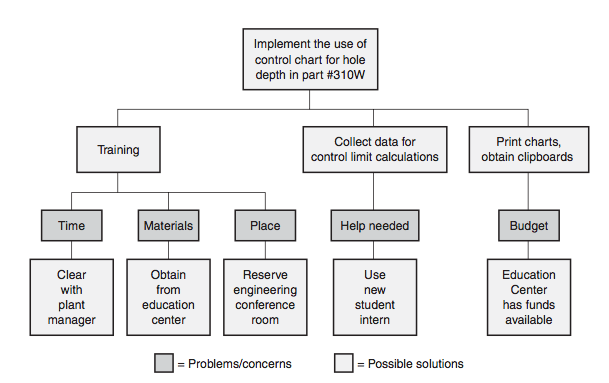
\includegraphics[width=120mm]{imagenes/PDPC.png}
	\caption{PDPC}
	\label{fig:PDPC}
\end{figure}

Diagrama de árbol para ilustrar problemas, anticiparse a ellos y listar soluciones posibles.

\subsection{Risk Priority Number}

Calculado de los datos FMEA: severidad, ocurrencia y detección. RPN = S x D x O. RPN ayuda a determinar el potencial riesgo y a ayudar al \textit{project team} para priorizar los items sobre los que trabajar primero.

\subsection{Sampling Plan}

Hacer muestreos en base a factores: velocidad de la linea, tecnología disponible, numero de personas disponible, expectativa del consumidor, ... 
Consiste en coger un numero de muestras aleatorio que representen al conjunto del lote de fabricación.
Juran dijo que la inspección 100\% es solo el 80\% de efectiva.

\subsection{Diagrama SIPOC}

Definir procesos y sus limites. Identificar los outputs de los procesos, incluyendo datos, servicios, productos, información, registros... Ve a la columna de customers, para saber quien recibe qué output. Vuelve a la columna de Suppliers para identificar cuales son los internos y cuales los externos y cuales son sus inputs.

\subsection{Tree Diagram}

Ayuda a romper el topic general en un numero de actividades que contribuyen entre sí. El \textit{team project} debe dar entre 2 y 5 topics que contribuyan con el topic general, y la idea es ponerlos en línea horizontal. Se continua la rama del árbol hasta que no sea práctico. Se revisa el árbol consiguiendo seguridad de que trabajar cada item puede mejorar el topic. Por lo que el árbol resultante provee actividades específicas que contribuyen al topic general.

\begin{figure}[ht!]
	\centering
	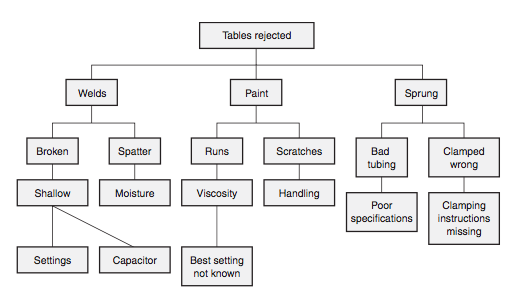
\includegraphics[width=120mm]{imagenes/TreeDiagram.png}
	\caption{Tree Diagram}
	\label{fig:TreeDiagram}
\end{figure}

\subsection{Tool Review}

La fase de definición se centra en determinar el alcance de las mejoras del proyecto y de los recursos y calendario necesitado para ejecutar el proyecto. Hay mucha herramientas para ayudar en la definición y gestión del proyecto, incluyendo Gantt. Las herramientas y el nivel de detalle debe ser basado en el tamaño del proyecto.

\section{Resultados de negocios por proyectos}

Los resultados de negocios pueden ser mostrados de muchas maneras y en muchos niveles de detalle. Las medidas de los resultados de los proyectos deben ser identificadas durante la fase inicial y redefinidas mientras el proyecto avance. Las \textit{performance measures (medidas de desempeño)} están relacionadas con el negocio, proyectos o procesos y son expresadas a través de \textit{balanced scorecard} o \textit{rendimiento de metas establecidas}.

Por un lado, las \textit{balanced scorecard} requieren que la organización evalúe su actuación en 5 áreas principales: financiera, cliente, procesos internos, aprendizaje y crecimiento. Así se consigue alinear la visión de la empresa con las metas, asegurando que ningún área sobresalga del resto.

Por otro lado, el rendimiento de las metas establecidas consiste en establecer metas, y revisar la consecución de las mismas a lo largo del tiempo. Siempre deben ser cuantificables. Ejemplo: Incrementar facturación 10\% más sobre el año anterior.

Para medir, se utiliza \textit{Cost performance index (CPI)}, que consiste en establecer un ratio entre el coste/beneficio entre los escenarios actual/futuro. \textit{Schedule performance index (SPI)} mide la eficiencia del calendario también por ratio: objetivos logrados vs planificados.
	
\subsection{Process Performance}

Calcular las métricas \textit{de rendimiento del proceso} como: Defectos por Unidad (DPU), Rolled Throughput Yield (RTY), coste de mala calidad (COPQ), defectos por millón de oportunidades (DPMO), niveles sigma, indices de capacidad de proceso. A través de estas métricas, conduce la toma de decisiones de los proyectos.

La palabra defecto no está permitida ser utilizada en relación con productos y servicios.

\begin{itemize}
	\item Defects per unit (DPU): número total de defectos dividido por el numero total de productos producidos en un periodo temporal.
	\item Defects per million opportunities (DPMO): calcular el numero de oportunidades, es necesario encontrar el número de caminos que hay para que cada defecto ocurra.
	\item Rolled throughput yield (RTY): RTY aplica al rendimiento desde series de procesos y es encontrado por multiplicidad de procesos individuales.
	\item Sigma levels: Supón la tolerancia de una dimensión en 5 $\pm$ 0.012 [4.988 - 5.012]. Los datos dicen que el proceso es $\sigma = \pm$0.004. 3$\sigma$ caben dentro de tolerancia ya que 3 x $\pm$0.004 = $\pm 12$.
	\item Process capability indices:
	\begin{itemize}
		\item $C_p$: es el ratio de tolerancia $6\sigma$ 
		\item $C_pk$: es el mejor de las medias USL dividida por 3 sigma (o la media) menos el LSL dividido por 3 sigma. El mayor valor $C_pk$, el mejor.
		\item $C_r$: el ratio de 1 dividido por $C_p$
	\end{itemize}
\end{itemize}

\subsection{Communication}

Define y describe técnicas de comunicación usadas en la organización: top-down, bottom-up, horizontal.

La transmisión de información implica un cambio del comportamiento, al menos es lo esperado. Es el sentido de comunicar algo en una organización. Es clave que quien dirija tenga buenas habilidades comunicativas, pero todo el mundo las necesita ya que hay diferentes flujos de comunicación.

\begin{itemize}
	\item Top-down flow: Las instrucciones que da el de arriba hacia abajo, la comunicación de las políticas, el \textit{feedback} de las actuaciones.
	\item Bottom-up flow: desde los operadores de línea a supervisores, encargados y así hacia arriba. Es importante considerar sugerencias.
	\item Horizontal: la mas útil para conseguir resultados rápidos y efectivos. Puede ocurrir que los escalones jerárquicos superiores sientan han sido saltados ya que las decisiones se están arreglando un nivel más abajo entre varios.
\end{itemize}

\section{Team Dynamics and Performance}
\subsection{Team Basics}

\begin{quote}
There is no ``I" \ in ``team".
\end{quote} Equipo es un conjunto de esfuerzos individuales. Para aprovechar lo mejor de cada individuo, hay que conocer las fortalezas, roles y responsabilidades de cada uno, así como el alcance de la tarea. ¿Cómo formar un equipo? ¿cómo organizar meetings? ¿cómo gestionar proyectos? ¿cómo conseguir las metas deseadas. A la hora de comenzar, la idea es marcar las metas, hitos, objetivos y que cada miembro del equipo entienda las expectativas. Generar un orden del día flexible.

En todas las reuniones hay que tener las metas, objetivos y alcance/límites visibles para no perderse.

\subsection{Team Formation}

De 5 a 9 miembros, 7 es el tamaño perfecto, con habilidades complementarias para conseguir metas y objetivos para el equipo. Debe ser conducido por el tamaño y alcance del proyecto. Si se puede, se hacen subdivisiones de proyectos.

El equipo debe incluir expertos y a los grupos de interés. Un proyecto no puede ser implementado si parte de los grupos de interés no están presentes en el desarrollo del mismo.

La interacción es buena, pero puede ser perjudicial. Si hay gran diversidad entre los perfiles, producen mejores interacciones. Los externos suelen hacer preguntas a los que están cerca del proceso. Estas reuniones deben ser moderadas para no machacar haciendo demasiadas preguntas.

\subsection{Virtual teams}

Innovación debido a las nuevas tecnologías. A través de internet se comparten datos virtualmente y hacemos entrevistas vía videoconferencia. Reduce costos.

\subsection{Team Stages and Dynamics}

Definir y describir las etapas de la evolución del equipo: forming, storming, norming, performin, adjourning y recognition. Identificar y ayudar a resolver dinámicas negativas: overbearing, dominante, reluctant participant, la aceptación incuestionable de las opiniones como un hecho, pensamiento grupal, feuding, floundering, the rush to accomplishment, attibution, discounts, digresions y tangents.

Los proyectos fallan por falta de trabajo en equipo. Según B.W. Tuckman's las etapas típicas son: forming, storming, norming and performing. Aunque aquí vamos a meter dos mas.

\begin{enumerate}
	\item Forming: que los miembros se conozcan. Que no sea un grupo inmaduro. Que haya sentido de pertenencia al grupo. Orgulloso de estar en el grupo. Intentar ayudar a los demás. Ser positivo ante los discussion topics. Que no sea una gran carga de trabajo. Los miembros deben estar orientados hacia metas. Asegurarse de que los miembros entienden roles y responsabilidades. En conjunto, esta fase es como una \textbf{luna de miel}.
	\item Storming: los miembros dan ideas. Entendimiento y alcance de los miembros, sus roles y responsabilidades. Se cogen ideas y se empieza a debatir. Los desacuerdos ralentizan al grupo. No se saca mucho trabajo adelante. Procurar que no haya interacciones negativas, ni completos desacuerdos.
	\item Norming: los miembros deben resolver sus conflictos. Los miembros aceptan ideas para avanzar. Mucho trabajo sale adelante. Empiezan a funcionar como equipo. Los miembros empiezan a confiar unos en otros. 
	\item Performing: Equipo efectivo, habilidades complementarias, se crea sinergia. Cada uno hace lo que mejor sabe hacer.
	\item Transitioning/Adjourning: Se disuelve el equipo. Los miembros vuelven a otras actividades de su trabajo. Si el proyecto continua con un alcance adicional, algunos miembros deben ser cambiados. La dinámica cambia y vuelve a las primeras etapas. 
	\item Recognition: reconocer la labor: notas de agradecimiento, e-mail, newsletter, una reunión con todos los empleados, certificados, bonus o un extra económico.
\end{enumerate}

\subsubsection{El liderazgo por etapas: Team Leadership}

\begin{enumerate}
	\item Forming (directing): supervisor directa, exhibe comportamiento de director. Da instrucciones de que hacer cuándo, dónde y cómo. Escucha el \textit{feedback}, anima al equipo, explica los roles y responsabilidades, identifica las oportunidades para desarrollar habilidades.
	\item Storming (coaching): supervisor directa, exhibe comportamiento de director. Empieza comportamiento de ayuda. Escucha más al equipo.
	\item Norming (supporting): Baja el nivel de comportamiento como director y más de ayuda. Anima a tomar decisiones sobre las responsabilidades. Ayuda a mover la actuación de etapa antes de que vuelvan a una etapa anterior.
	\item Performing (delegating): desde que el equipo es maduro, se reduce el nivel de dirección y de soporte en las funciones del día a día. Todavía monitoriza las metas y las actuaciones del equipo. Observa cualquier cambio en la dinámica debido a cambios importantes. 
\end{enumerate}

\subsubsection{Negative Team Dynamics}

\begin{itemize}
	\item Overbearing member(s). Pocos hablan, muchos escuchan. Causas: miembros demasiado influyentes. Medidas: round-robin desde el miembro influyente hacia el resto.
	\item Dominant member(s). Reunión caótica, difícil de escuchar o entender. Causas: dominantes interrumpen al resto constantemente. Medidas: Estructurar el orden del día para que todos hablen. Hacer moderación efectiva. Round-robin.
	\item Floundering. El equipo se encuentra en proceso o está actuando de una manera inestable y vacilante. Causas: Falta de dirección de equipo. Miembros abrumados/sobrecargados. Aplazamiento de las decisiones de equipo. Medidas: más dirección en las primeras etapas. El líder debe ser visible durante la reunión y toma de decisiones.
	\item Participante reacio. Falta de participación. Desinterés. Causas: no tiene interés en los resultados de equipo. Está intimidado por otros miembros. Tiene miedo de perder su trabajo u opiniones. Medidas: Los líderes ayudan a los miembros a que activen su participación.
	\item Aceptación incuestionable de opiniones como hechos. Presentación de datos sin análisis. Causas: razones culturales, falta de gestión por hechos. Medidas: pedir datos.
	\item Groupthink. No hay desacuerdos. Dudas expresadas en ambiente privado. Causas: miedo. Medidas: traer gente que no sea del equipo a participar. Cambiar los roles.
	\item Feuding (riñas, reñirse). Baja moral de equipo, bajo progreso. Causas: resolución de conflictos no efectivos. Falta de respeto entre miembros. Medidas: Disciplina. Confrontar en privado. 
	\item Prisa por el logro. Falta de datos. Análisis inconsistente. Causas: Plazos absurdos. Miembros novatos buscando metas a corto plazo. Medidas: Datos, análisis y significado estadístico. Pedir alternativas. Revisar plazos.
	\item Attribution. miembros hacen referencias casuales. no buscan explicaciones. Se dejan llevar por las emociones. Causas: igual que prisa por el logro. Medidas: Poner en tela de juicio lo que han dicho.
	\item Discounts. Opiniones ignoradas. No se escuchan. Sarcasmo. Medidas: alentar el respeto. preguntar por la clarificación de las opiniones.
	\item Disgressions and tangents. Discusión fuera del alcance. Distracciones. Causas: Cuestiones culturales, falta de liderazgo. Medidas: Hacer cumplir la agenda. 
\end{itemize}

\subsection{Team Roles and Responsibilities}

\begin{tabular}{p{1.5cm}|p{3cm}|p{4cm}|p{7cm}}
	\hline Rol & Candidato & Training/Background & Responsabilidades principales \\ 
	\hline Executive sponsor & Líder responsable de la unidad de negocio para beneficios y perdidas (de nivel de director o superior). & Conceptos six sigma, overview, definición de operaciones. & Fijar dirección y prioridades para la organización Six sigma. Asignar los recursos de los proyectos. Fijar la visión Six Sigma. Monitorizar el progreso sobre el programa completo. Iniciar programas de incentivos. Recompensar los proyectos exitosos.  \\ 
	\hline Champion & Managers de nivel superior & Conceptos Six Sigma, estrategias, herramientas y métodos, operaciones. Especial énfasis en herramientas de gestión. & Asignar recursos a proyectos. Determinar el criterio para la selección de proyectos. Quitar barreras ocultas para el éxito del proyecto. Aprobar el proyecto completo. Implementar cambios. \\ 
	\hline Process Owner & Persona responsable y que controle la ejecución y resultados del proceso. Sponsor o Champion puede ser este perfil al mismo tiempo. & Conceptos Six Sigma, estrategias, herramientas, metodología, definiciones. & Selecionar team members. Asignar recursos a proyectos. Proveer conocimiento del proceso. Revisar cambios del proceso. Aprobar cambios. Implementar cambios. Asegurar que las mejoras son sustanciales. \\ 
	\hline Master Black Belt & Quien sepa de Six Sigma, estadística, cambio, riesgo, inversión, gestión de proyectos, haya dado formación, coaching & Six Sigma BoK, Lean synergy, management, change agen skill. & Enseñar Six Siggma, utilizar recursos, formular estrategia Six Sigma, monitorizar proyectos, proveer entrenamiento/coaching, trabajar con Champions y Procesos, quitar barreras, ayudar a expertos, revisar y aprobar proyectos, compartir lo aprendido. \\
	\hline Black Belt & Similar a Master Black Belt. & Similar a Master Black Belt. & Dirigir y gestionar proyectos Six Sigma, utilizar recursos a su disposición, calculo de ROI, payback, trabajar 6 proyectos/año, Seguir DMAIC process, quitar barreras, actualizar proyecto, hitos y su gestión, revisar proyectos completados, compartir lo aprendido.\\
	\hline Green Belt& Conocimiento de Six Sigma y estadística básica y mejora de procesos. & Six Sigma BoK, Lean Synergy, presentation y comunication skills. & Ayuda en proyectos Six Sigma. Dirección pequeños proyectos y ROI (retorno de inversión), Seguir DMAIC y aplicar estadística, revisar la consecución con los Black y Master Black, identificar estancamientos del proyecto, identificar y reportar barreras, compartir lecciones aprendidas con el resto. \\
	\hline Project team member & Seleccionado por el Process Owner y entrenado en Six Sigma, calidad, estadística básica y técnica de mejora de procesos. & Metodologías Six Sigma, herramientas de calidad, mejora de procesos, trabajo en equipo. & Ayuda y contribución a proyectos six sigma, participación en la definición del alcance, proveedor de inputs, brainstorm ideas, sigue proceso DMAIC y aplica herramientas apropiadas, revisa la consecución con Green Belt, provee inputs a los Belts y al process owner. \\
	\hline Yellow Belt & Algo de Six Sigma, interés, necesidad de desarrollar conocimiento fundamental & Metodologías Six Sigma, herramientas de calidad, mejora de procesos & Seguimiento de proceso DMAIC aplicando herramientas adecuadas, ayuda a la gestión, sugerencias para futuros proyectos, usa procesos y herramientas en el lugar de trabajo. \\
	\hline 
\end{tabular} 

\subsection{Team Tools}

\subsubsection{Brainstorming}
Se compone de dos fases: creativa para generar ideas y de evaluación para ver la utilidad y aplicabilidad de las tareas. Al menos 10 minutos de descanso entre las dos fases.

Durante la fase creativa: no distracciones o críticas, mente abierta a cualquier posibilidad aunque sea idea loca. La meta es conseguir el mayor número de ideas posibles.

Don'ts: no criticas, alagos ni preguntas, ideas locas son bienvenidas, no esperes turno, la cantidad de ideas es mas importante que la calidad, construir sobre ideas anteriores es bueno.

Hay muchos métodos para evaluar las ideas generadas, por ejemplo: construir un \textit{Affinity Diagram} para ayudar en la evaluación del proceso. Importante: no ser demasiado crítico con las ideas locas, ya que un cambio en tecnología o métodos es posiblemente la solución y lo que ocurre es que es muy criticado, ya que en la organización eso de cambiar la manera de hacer las cosas no es común.

Evitar cosas tales como: no seas ridículo, aparquemos esta idea por ahora, esto no funcionará aquí, es un cambio demasiado radical.

En la practica, brainstorming se utiliza para dar posibles soluciones a problemas. Hay que tener el problema bien acotado y definido para poder llevar a cabo un buen Brainstorming.
Para acotar el problema, al equipo se le dan unos minutos para que piensen sobre él, si no tienen ideas, aún así se le invita a participar en la segunda ronda. Lo que no se permite son las críticas.
Se pueden desarrollar ideas citadas por miembros.

Después de un par de rondas, se deben disolver los equipos, aunque permitir a los ex-miembros que vengan a seguir apuntando ideas (ya de manera mas individual). Tampoco hay que alargar esto, puede ser contraproducente.

\subsubsection{Nominal Group Technique}

Cuando algunos miembros hablan mas que otros, el tema es complicado o genera controversia se utiliza NGT para aliviar presión. 
Similar a Brainstorming, facilitator explica las normas, team leader presenta el tema. 10 - 15 minutos para sentarse, pensar y generar ideas. No deben haber interacciones entre ellos. Las ideas se escriben donde todos las puedan leer. No se aprueba juicios sobre las ideas o criticas. Buscar claridad y eliminar redundancia.

\subsubsection{Multivoting}

Esta herramienta complementa NGT. Las ideas consolidadas son numeradas por letras alfabéticamente ordenadas y se votan cuales son el TOP 5 que tienen más influencia sobre el problema. Se priorizan las más importantes de todas.

\subsection{Team Communication}

Identifica y usa métodos apropiados de comunicación.
\pagebreak[4]
\part{Medición}
 
\section{Process Analysis and Documentation}

\subsection{Process Maps and Flowcharts}

ISO 9001 define un proceso como un conjunto de actividades interrelacionada que transforman inputs en outputs.

Los procesos se entienden fácil haciendo flowcharts con formas y símbolos.

ISO 5807:1985 ayuda a utilizar con criterio los símbolos para los flowcharts.

Mapping process es el primer paso en la mejora de procesos. Herramientas para el análisis de riesgo (PFMEA) empiezan con el mapeado de los procesos.

Los flowchart muestran en cada proceso, incluyendo inputs, puntos de decisión, y outputs, además incluyen información adicional del proceso, pasos, costes, tiempos de setup, tiempos de ciclo, tipos de defectos que pueden ocurrir, ....

Hay varios tipos de flowchart: simples, cross-functionals (swim lane).

Pasos para crear un flowchart:

\begin{enumerate}
	\item Determinar los límites del proceso (sus inputs y sus outputs)
	\item Determinar los pasos del proceso a través de brainstorming, walking the process.
	\item Construir la secuencia del proceso.
	\item Dibujar el flowchart.
	\item Verificar que le flowchart está correctamente construido.
\end{enumerate}

Flowcharts muestran pasos redundantes, que no añaden valor e innecesarios. 

Errores comunes en el diseño de flowcharts: representación del equipo para el proceso es inadecuada o inapropiada. alcance borroso, falda de coordinación con otros procesos. La gente que sigue el proceso. Se pierde mucho tiempo creando el flujo perfecto.

\subsection{Written procedures and Work Instructions} 

Los procedimientos son escritos para describir: que ocurre durante el proceso, porqué se hace (razón de negocio), dónde se hace (localización) y cuando es realizado (disparador).

Las instrucciones de trabajo explican: quién hace qué (personal con determinadas skills), y cómo es hecho (los pasos). 

Cuando no hay un procedimiento interno especifico para una actividad particular y no se requiere de su estandarización, es aceptable que la actividad se conduzca a través de un método. Un método es un proceso no-escrito que debe ser seguido.

Para determinar cuales procesos han de ser documentados, la organización debe considerar: 

\begin{itemize}
	\item Efecto en calidad
	\item Riesgo de la insatisfacción del cliente
	\item Riesgo económico
	\item Efectividad y eficiencia
	\item Competencia del personal
	\item Complejidad del proceso
\end{itemize}

Las instrucciones de trabajo pueden ser documentadas como: Instrucciones escritas, checklists, flowcharts, fotografías, dibujos, videos, pantallas electrónicas.

\subsection{Process Inputs and Outputs}

Cada proceso tiene inputs, outputs y loops de feedbacks. El feedback hace falta para mejorar el proceso. Ejemplos de \textbf{inputs}: necesidades, ideas, expectativas, requerimientos, información, datos, documentos, recursos. Ejemplos de \textbf{outputs}: diseños, decisiones, resultados, medidas, productos, servicios, propuestas, soluciones, autorizaciones, actuaciones.

A la hora de hacer un Chart para un proceso hay que tener en cuenta: Primero identificar Inputs/outputs. El mapa global de procesos debe incluir al SIPOC (Suppliers, inputs, processes, outputs, customers). 

Los pinputs son medidos y las variaciones controladas a través de su respuesta y = f(x). Los efectos de las variaciones se determinan a través de \textit{Fishbone Diagram} con las categorías Measurement, Material, Personnel, Environment, Methods y Machines.

\begin{figure}[ht!]
	\centering
	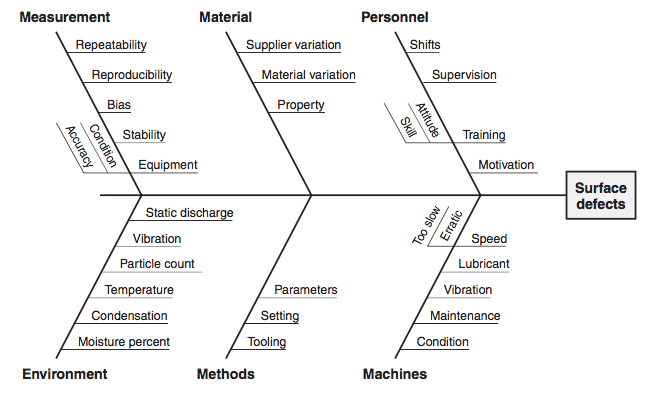
\includegraphics[width=120mm]{imagenes/Cause-and-effectDiagram.png}
	\caption{Cause-and-effect Diagram}
	\label{fig:CauseandeffectDiagram}
\end{figure}

Para poder generar el diagrama \ref{fig:CauseandeffectDiagram} es recomendable hacer \textbf{Brainstorming}, para priorizar, utilizar \textit{Multivoting} o \textit{nominal group technique} (NGT).

La convergencia tiene que lograrse, la idea para alentar a la participación es decir cosas como: he probado dos refrigerantes diferentes y el resultado en superficie en cuanto a defectos, es el mismo. También vale: hemos encontrado que el fabricante recomienda una humedad relativa del 55 al 60\%.

Ejemplo: datos sobre inspecciones finales.

\begin{tabular}{|c|c|c|c|c|c|}
	\hline Código defecto & Descripción & Ocurrencias & Criticalidad & Peso & Puntuacion ponderada \\ 
	\hline A & Arañazos & 15 & Menor & 10 & 150 \\ 
	\hline B & Manchas & 17 & Menor & 10 & 170 \\ 
	\hline C & Mancha en etiqueta & 12 & Menor & 10 & 120 \\ 
	\hline D & Abolladura & 14 & Mayor & 25 & 350 \\ 
	\hline E & Unidad no funcional & 6 & Critico & 100 & 500 \\ 
	\hline F & LED roto & 7 & Critico & 100 & 700\\ 
	\hline G & Falta de tornillo & 3 & Mayor & 25 & 75 \\ 
	\hline 
\end{tabular} 

Siempre se ordenan de mayor a menor a la hora de representarlos, salvo la sección Otros, que suele ser la misma. Tanto para representar el numero absoluto como para representar el peso. Fijándonos en la figura \ref{fig:ParetoPlot} tenemos el primer item en un caso Manchas, y en otro LED roto. 
Si ploteamos Pareto en relación 80:20 tenemos:

\begin{figure}[ht!]
	\centering
	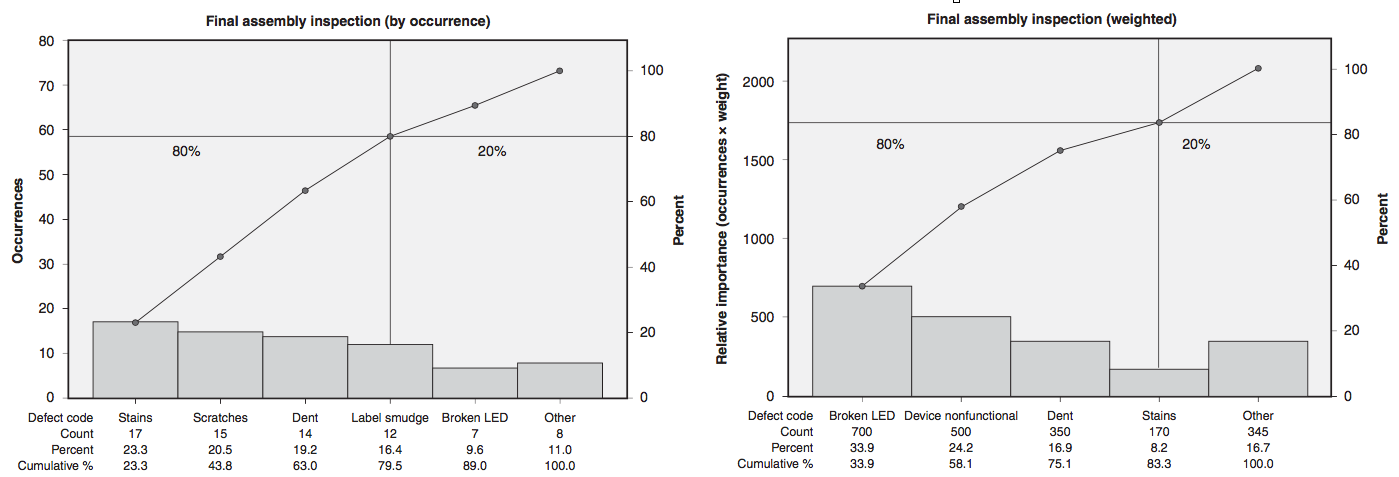
\includegraphics[width=180mm]{imagenes/ParetoPlot.png}
	\caption{Pareto Plot}
	\label{fig:ParetoPlot}
\end{figure}

\textit{Measles charts} son utiles para productos largos, como automóviles, y donde las oportunidades de defectos son altas.

\subsection{Relationship Diagram}

El diagrama de relaciones es utilizado para mostrar el grado de relación entre variables, causas y efectos. Consiste en poner diferentes defectos y ver como acciones que se pueden controlar o no, afectan a ello.

\begin{figure}[ht!]
	\centering
	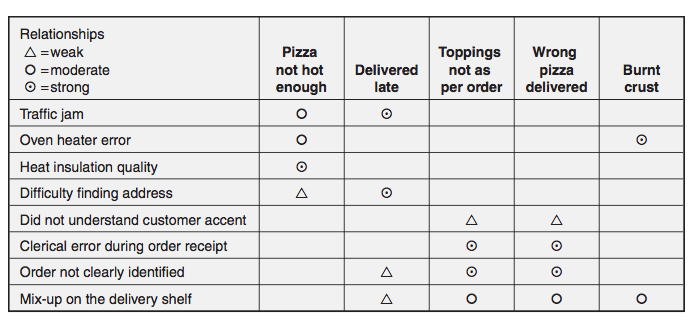
\includegraphics[width=120mm]{imagenes/RelationshipMatrix.png}
	\caption{Relationship Matrix}
	\label{fig:RelationshipMatrix}
\end{figure}

\section{Probability and Statistics}

\subsection{Basic Probability Concepts}

\textbf{Complementation Rule}: La probabilidad de que el evento A no ocurra es: 1 - la probabilidad de que ocurra. 

\begin{figure}[ht!]
	\centering
	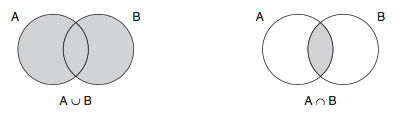
\includegraphics[width=80mm]{imagenes/DiagramaVenn.png}
	\caption{Diagrama Venn}
	\label{fig:DiagramaVenn}
\end{figure}

\textbf{Probabilidad condicional}: La probabilidad de que un evento se de, cuando otro evento se ha dado. $P(B\mid A) = P(A \& B)/P(A)$

La probabilidad de sacar un 4 tirando un dado es 1/6. Y de sacar un 6 también 1/6. Por lo tanto, la probabilidad de sacar un 4 o un 6 es: 1/6 + 1/6 = 1/3.

En una organización hay dos máquinas de inyección cy la probabilidad de funcionamiento es del 0.8, la probabilidad de que la producción semanal salga es: \newline 
$P(A \bigcup B) = P(A) + P(B) - P(A \bigcap B)$, al no ser eventos mutuamente exclusivos \newline $P(A \bigcup B) = 0.8 + 0.8 - (0.8 * 0.8) = 1.6 - 0.64 = 0.96$. \newline Si fueran mutuamente exclusivos, $P(A \bigcup B) = P(A) + P(B)$

\textbf{Ley multiplicativa}: en eventos dependientes.

Una producción de 50 unidades, tiene 10 defectuosas. Tres son muestreadas aleatoriamente. ¿cual es la probabilidad de que las tres sean defectuosas?
La probabilidad sería 10/50 para la primera, 9/49 para la segunda y 8/48 para la tercera, ya que las tres tienen que ser defectuosas: 0.6\%.

\textbf{Ley multiplicativa}: en eventos independientes.

Un ensamble necesita 2 componentes, la probabilidad de que A funcione es 0.7, y la de B es 0.8. Cual es la probabilidad de que el ensamblaje funcione? $P(A \bigcap B) = 0.7*0.8 = 0.56$

\textbf{Permutaciones y combinaciones}. \newline La permutación es una disposición ordenada de \textit{n} objetos distintos. Ocurre cuando AB es diferente de BA. El número de formas de ordenar la disposición: \textit{r}. Se designa nPr.
\begin{equation}
nPr = \frac{n!}{(n-r)!}
\end{equation}

Este caso vale para: la palabra \textit{sigma} tiene 5 letras. ¿De cuantas maneras diferentes se pueden combinar las 5 letras? 5P5 = 5! = 120.

El número distinto de combinaciones de \textit{n} objetos tomados \textit{r} cada vez. Esto ocurre cuando AB es igual que BA. nCr

nCr = $\frac{n!}{r!(n-r)!}$
Este caso vale para: Tienes 10 personas y quieres enviar a 3 a formarse para un puesto. ¿cuántas combinaciones posibles hay? 10C3. $\frac{10!}{(10-3)!3!} = 120$

\subsection{Teoría del límite central}

CLT no es más que el error medio cuadrático. Se basa en

\begin{enumerate}
	\item La media de la distribución de muestra es igual a la media de la población.
	\item La varianza de la distribución es igual a la varianza de la población.
	\item La población original se distribuye bajo campana.
\end{enumerate}

Es aplicable para SPC control charts, X, R.

\begin{tabular}{|c|c|c|}
	\hline  & Sample & Population \\ 
	\hline Size & n & N \\ 
	\hline Mean & x & $\mu$ \\ 
	\hline Standar dev & s & $\sigma$ \\ 
	\hline 
\end{tabular} 

\section{Statistical Distributions}

\begin{tabular}{|c|c|c|c|}
	\hline Nombre & Formula & Media & Varianza \\ 
	\hline Normal & $P(x)=\frac{e^\frac{-(x-\mu)^2}{2\sigma^2}}{\sigma \sqrt{2 \pi}} $  & $\mu$ & $\sigma^2$ \\ 
	\hline Exponential & $P(x)=\lambda e^{-\lambda x} $ & $1/\lambda$ & $1/\lambda^2$ \\ 
	\hline Binomial & $P(x)= \frac{n!}{x!(n-x)!}p^x(1-p)^{n-x}) $ & np & np(1-p) \\ 
	\hline Poisson & $P(x)= \frac{e^{-\lambda}\lambda^x}{x!}$ & $\lambda$ & $\lambda$ \\ 
	\hline Hipergeometrica & * & $\frac{nd}{N}$ & $\frac{nd(N-d)(N-n)}{N^3-N^2}$ \\ 
	\hline 
\end{tabular} 

\subsection{Binomial}

Se aplica para distribuciones que tienen dos estados: Bueno/malo, aceptado/rechazado, conformidad/no conformidad, éxito/fallo.

Ejemplo: Se cogen 5 muestras, de un conjunto donde el 10\% tienen defectos, cual es la probabilidad de que la muestra elegida al azar tenga un defecto? 

\begin{figure}[ht!]
	\centering
	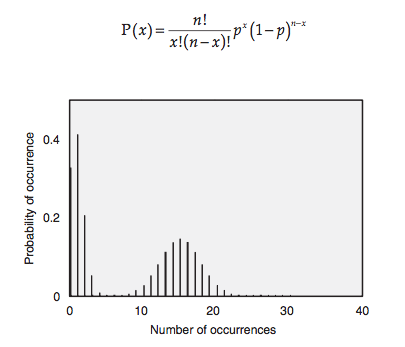
\includegraphics[width=90mm]{imagenes/BinomialDistribution.png}
	\caption{Binomial Distribution}
	\label{fig:BinomialDistribution}
\end{figure}

Se sustituye en \ref{fig:BinomialDistribution}, x = 5, n = 1, p = 0.1. BINOMIDST en Excel.

Tirar una moneda vale para esto. Tirar una moneda 60 veces, ¿cual es la desviación estándar? $\sigma = \sqrt{np(1-p)} = 3.872$ 

\subsection{Poisson}

Representa la distribución de una probabilidad discreta: número de defectos en una unidad de ensamblaje. Numero de defectos en una superficie pintada, Número de bugs en código de software.

Se habla de DPO (\textit{Defects per opportunity}) o DPMO (\textit{Defects per million opportunities}).

\begin{equation}
P(x)= \frac{e^{-\lambda}\lambda^x}{x!}
\end{equation}

El número de defectos en una unidad de ensamblaje tiene una distribución de Poisson con $\lambda = 5$. Encuentra la probabilidad de que la segunda unidad producida  tenga menos de dos defectos.

\begin{equation}
P(x < 2) = P(x=0)+P(x=1)
\end{equation}

\begin{equation}
P(x = 0) = \frac{e^{-5}5^0}{0!} \approx 0.006
\end{equation}

\begin{equation}
P(x = 1) = \frac{e^{-5}5^1}{1!} \approx 0.034
\end{equation}

\begin{equation}
P(x < 2) = 0.006 + 0.034 = 0.04
\end{equation}

Un un proceso de una máquina de ensambles tiene un ratio de defecto del 10\%. Cual es la probabilidad de que 50 unidades tengan 5 defectuosas? n = 50, p = 0.1 $\longrightarrow \lambda = 50*0.1 = 5$, x = 5 (uds defectuosas).

\begin{equation}
P(x) = \frac{e^{-\lambda}\lambda^x}{x!} = \frac{e^{-5}5^5}{5!} = 0.175 \approx 18\%
\end{equation} 

\subsection{Distribuciones normales}

Distribuciones continuas, estilo peso, masa, tiempo. 

Ejemplo: un restaurante de pisa procesa pizzas bajo una distribución normal. Una muestra aleatoria muestra 30 minutos de proceso y 5 minutos de desviación standard. Estima el porcentaje de pedidos entre los 20 y los 30 minutos.

Buscar el valor Z, Z es el numero de desviaciones estandards que una medida se desvía de la media y se calcula tal que

\begin{equation}
Z = \frac{x - \mu}{\sigma} \longrightarrow Z(20) = \frac{(20-30)}{5} = -2
\end{equation}

\begin{equation}
Z = \frac{x - \mu}{\sigma} \longrightarrow Z(35) = \frac{(35-30)}{5} = 1
\end{equation}

Área a la derecha de -2 = 0.97724 \newline
Área a la derecha de +1 = 0.15865 \newline
Diferencia entre ambos= 0.8186 $\longrightarrow$ 82\% de los pedidos son procesados entre los 20 y los 35 minutos.


\subsection{Distribución Chi-cuadrado}

Si $w, x, y$ y $z$ son variables aleatorias de distribución normal standar la variable $f = w^2 + x^2 + y^2 + z^2$ tiene una distribución $\chi^2$
La distribución $\chi^2$ se aplica para test de proporcionalidad, conforme los grados de libertad de $\chi^2$ aumentan, se aproxima a una distribución normal. Propiedades 

\begin{itemize}
	\item $\chi^2$ no es negativo,
	\item $\chi^2$ no es simétrico,
	\item Hay muchas distribuciones $\chi^2$, una para cada grado de libertad,
	\item Los grados de libertad cuando se trabaja una población individual es $(n-1)$.
\end{itemize}


\subsubsection{Grados de libertad}

La cantidad de información que los datos pueden proveerte y que tu puedes aplicar para estimar valores de parámetros desconocidos y calcular sus variaciones.

\subsubsection{t-Distribution}

Si $x$ es una variable aleatoria con una distribucion normal y $y$ es una variable con una distribución $\chi^2$, entonces la variable definida es

\begin{equation}
 t = \frac{x}{\sqrt{\frac{y}{k}}}
\end{equation}

siendo k los grados de libertad de $\chi^2$. Cuando $k \longrightarrow \infty, t$, se aproxima a una distribución normal.

Propiedades importantes de la Student's t-distribution:
\begin{itemize}
	\item es diferente para diferentes tamaños de muestra,
	\item generalmente tiene forma de campana, aunque no siempre,
	\item la media es cero,
	\item la distribución es simétrica respecto de la media,
	\item La varianza es mayor que 1, y se aproxima a 1,
	\item La population standard deviation es desconocida,
	\item La población es esencialmente normal.
\end{itemize}

Doce paquetes seleccionados aleatoriamente pesan: 7.3, 7.9, 7.1, 7.3, 7.4, 7.3, 7.0, 7.3, 7.7, 7.3, 7.1, 7.8 y según anuncia el paquete, es 7.5. 

Media: 7.375, EMC (desviacion estandar) $\sigma^2 = 0.2832$

\subsection{F-Distribution}

F-Distribution es el ratio de dos distribuciones $\chi^2$ con grados de libertad $v_1$ y $v_2$ respectivamente, comúnmente se usa para ANOVA.

\begin{figure}[ht!]
	\centering
	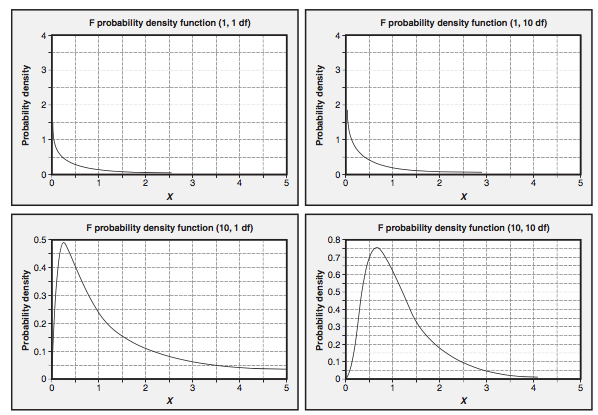
\includegraphics[width=120mm]{imagenes/F-Distribution.png}
	\caption{F-Distribution}
	\label{fig:F-Distribution}
\end{figure}

\section{Collecting and Summarizing Data}

\subsection{Tipos de datos y escalas de medida}

\begin{itemize}
	\item Nominal: los valores de la escala no son numéricos. Ej: color de ojos.
	\item Ordinal: Los intervalos entre valores son indeterminados. Ej: crítico, grave, medio, leve.
	\item Intervalo: Intervalos dentro de una misma escala. Ej: 40ºC y 20ºC, -10ºC y -30ºC.
	\item Ratio: Relacion entre dos valores. Ej: 10/5 = 64/32.
\end{itemize}

\subsection{Muestreo y recolección de datos}

Métodos: entrevistas cara a cara, encuestas, grupos de interés, mystery shopping, feedback del cliente, captación automática/manual de datos.

\subsubsection{Técnicas para asegurar la precisión de los datos y la integridad}

Causas comunes de errores de las técnicas: unidades de medida no definidas, ilegibilidad de caracteres escritos a mano, inadecuados sistemas de medida-discriminación, pérdida de precisión, sesgo emocional que distorsiona datos, inadecuado uso de técnicas de validación de datos, múltiples puntos de entrada de datos (inconsistencia), pobres instrucciones que generan entrada errónea de datos, terminología ambigua.

Minimizar errores: utilizar 5W1H (what, where, who, when, why and how), calendario de calibración para equipos de recogida de datos, R\&R (repitibilidad y reproducibilidad), metadatos interesantes (hora, quien graba el dato, equipo utilizado), usar test adecuados para quitar valores outliers, training para la recolección, transformación análisis e interpretación de los datos.

\textbf{Tipo de muestreo}: random, sequential (test destructivos), stratified (aleatorio pero atendiendo a una característica: diferente máquina, diferente lote, diferente proceso).

Random y stratified sampling son aplicables a muchos sectores.

Cuando los datos se meten a mano, lo suyo es generar una codificación-decodificación para evitar errores humanos.

\subsubsection{Check Sheets}

Se usan para revisar un proceso durante su ejecución. En ellas se precategoriza los potenciales resultados que se pueden obtener.

\begin{figure}[ht!]
	\centering
	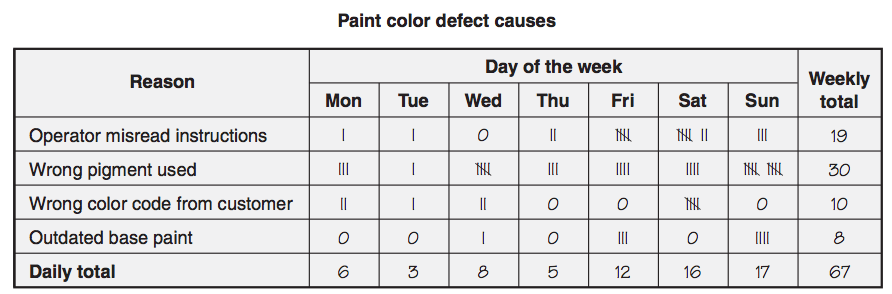
\includegraphics[width=120mm]{imagenes/CheckSheet.png}
	\caption{CheckSheet}
\end{figure}

Como elaborar una Check Sheet:

\begin{enumerate}
	\item Identifica las causas o condiciones de lo que va a ser recogido.
	\item Decide quien recogerá los datos, con que periodicidad y cómo.
	\item Crea una check sheet que funcione donde debe ser usada.
	\item Recoge los datos como diseño de asegurar consistencia y precisión de la información.
\end{enumerate}

\subsection{Estadísticas descriptivas}

\textit{Descriptiva}: presentar datos para facilitar el entendimiento.

\textit{Inferential}: analiza datos de una muestra para inferir propiedades de la población. 

Dispersión: 
\begin{equation}
s = \sqrt{\frac{\Sigma(x_i-x_{media})^2}{n-1}}
\end{equation}

Desviación estándar:
\begin{equation}
\sigma = \sqrt{\frac{\Sigma(x-\mu)^2}{N}}
\end{equation}

\subsubsection{Cumulative Frequency Distribution}

Representar la frecuencia y la frecuencia acumulada.

\subsection{Métodos gráficos}

\begin{tabular}{p{2cm}|p{2.5cm}|p{3cm}|p{5cm}|p{2.5cm}}
	\hline Nombre & Propósito & Aplicación & Interpretación & Facilidad de uso \\ 
	\hline Tally (registros) & Cantidad de \textbf{Defectos} por tipo de clase y/o intervalo & Usado para contar defectos por tipo, clase o categoría. & La concentración y propagación de la marca de registro indican aproximadamente la forma de distribución. Las marcas de cinco registros están tachadas como un grupo para contar fácilmente. Los grupos aislados de marcas de registro indican distribución desigual.. & Fácil de crear e interpretar.  \\ 
    \hline Distribución por frecuencia & Vista pictórica del numero de datos, su localización y su amplitud & Especialmente útil para muchos datos & La concentración de datos es vista como un pico, y los demás datos dan sentido a la amplitud de la curva. Unimodal, bimodal, multimodal (uno, dos, varios picos) & No es fácil de crear, pero sí fácil de interpretar. \\
    \hline (Stem-and-leaf Plot) Plot de tallo y hojas & Da información numérica y la distribución de la frecuencia & Útil para identificar rapidamente datos repetitivos en intervalos de clase. & Si los valores de datos no están justamente distribuidos, errores de medida o condiciones de medida pueden ser presentadas & Fácil de crear, difícil de interpretar. \\
    \hline Box-and-whisker Plot & Vista pictórica de mínimo, máximo, media, rango de cuartil. & Da más info pero mas difícil de interpretar. Valores fuera de limite fácilmente identificables. & Si la localización de la linea central de la caja está justo en el medio, los datos están distribuidos de manera Normal, sino, los datos estarán sesgados.  &  Fácil de crear e interpretar. \\
    \hline Scatter Diagram & Detectar correlación y asociación entre dos variables, causa efecto. & Usada para conocer la raíz de los problemas, hacer predicciones a través de la regresión & Para tener correlación, la relación debe ser lineal. Relaciones no lineales existen entre variables. Si aumenta izq a derecha, la relación es positiva. Si los datos no tienen inclinación, no están correlados. & Fácil de crear e interpretar. \\
    \hline run chart & Da un indicador visual de cualquier patrón no aleatorio & utilizado cuando se hace falta feedback a tiempo real & patrones como cluster, mixture, trend, oscilaciones son dibujados con los datos. p-valor identifica la significancia. p-valor inferior a 0.05 es mucha significancia & Fácil de crear e interpretar. \\
	\hline 
\end{tabular} 

\subsubsection{Stem-and-Leaf Plot}

Utilizado cuando los datos están agrupados.

\begin{figure}[ht!]
	\centering
	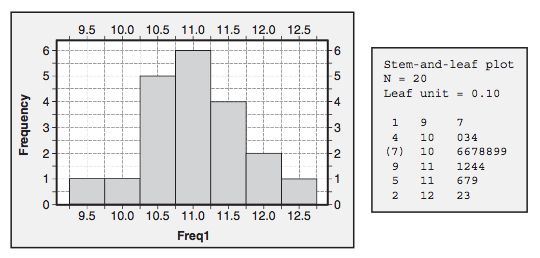
\includegraphics[width=120mm]{imagenes/Histograma.png}
	\caption{Histograma y stem-and-leaf plot}
	\label{fig:Histogramaystemandleafplot}
\end{figure}

Tres columnas: \textit{the leaves}: cada valor representa un dígito de una observación. Sgeún \ref{fig:Histogramaystemandleafplot}, el número leaf para cada observación sería: 1,3,7,4,3,2. \textit{the stem}: representa el dígito inmediatamente a la izquierda del dígito leaf en \ref{fig:Histogramaystemandleafplot}, según el rango, acumula los valores a representar. \textit{Counts} Si el valor mediano de la muestra está incluido en una columna, el valor se encierra entre paréntesis. 

\subsubsection{Box Plots}

\begin{figure}[H]
	\centering
	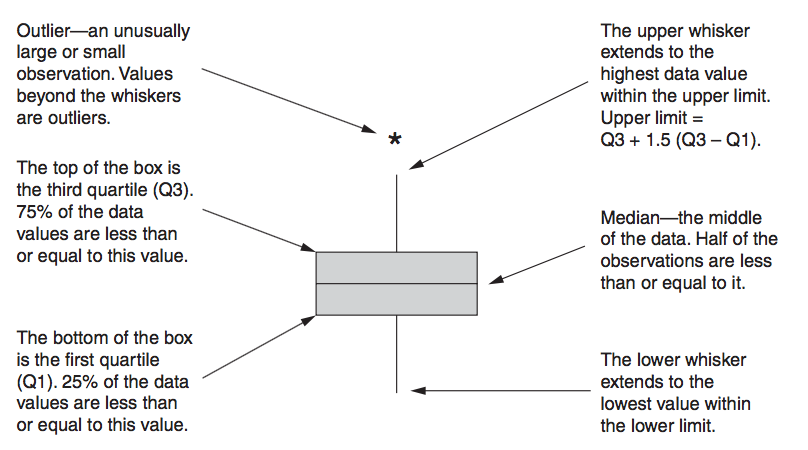
\includegraphics[width=120mm]{imagenes/Box-plot.png}
	\caption{Box-plot}
	\label{fig:Box-plot}
\end{figure}

\subsubsection{The Run Chart}

Es utilizada para identificar patrones en procesos. Todas las observaciones individuales se plotean en orden. Se pueden utilizar tendencias, oscilaciones, agrupaciones, ... 

La falta de firmeza en un proceso puede causar oscilación, el \textit{p-value} de la imagen es 0,78. Eso implica que no hay tendencia.

\begin{figure}[H]
	\centering
	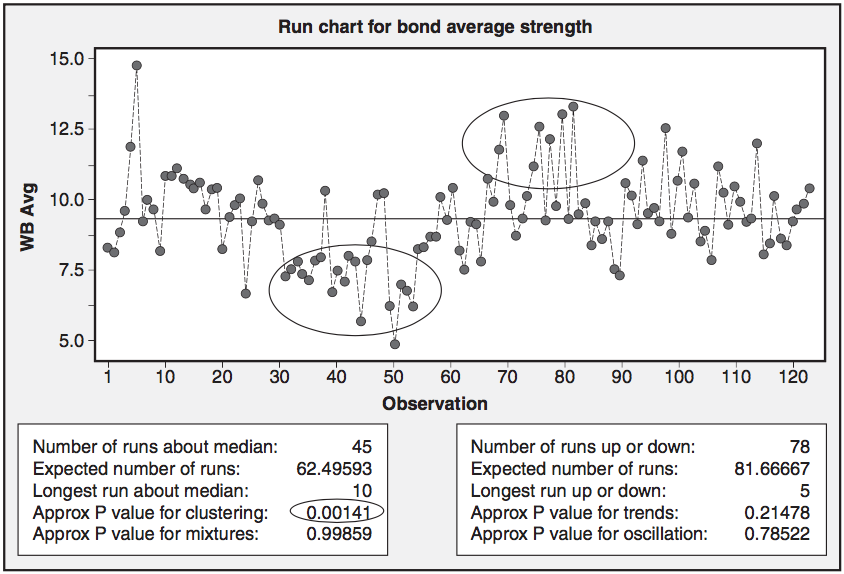
\includegraphics[width=120mm]{imagenes/Run-Chart-Analysis.png}
	\caption{Run Chart Analysis}
	\label{fig:Run-Chart-Analysis}
\end{figure}

El Run Chart es herramienta potente para enseñar como de estable está siendo un proceso.

\subsubsection{Scatter Diagrams}

Herramienta visual para ver relaciones entre dos variables, causa efecto y demás. 

\begin{figure}[H]
	\centering
	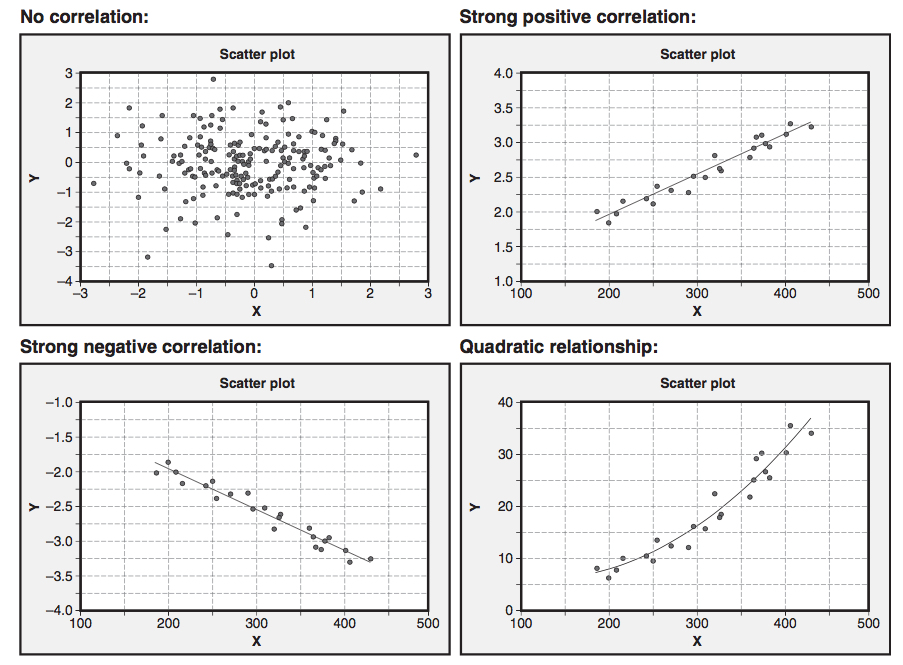
\includegraphics[width=120mm]{imagenes/ScatterPlot.png}
	\caption{Scatter Plot}
	\label{fig:ScatterPlot}
\end{figure}

\begin{figure}[H]
	\centering
	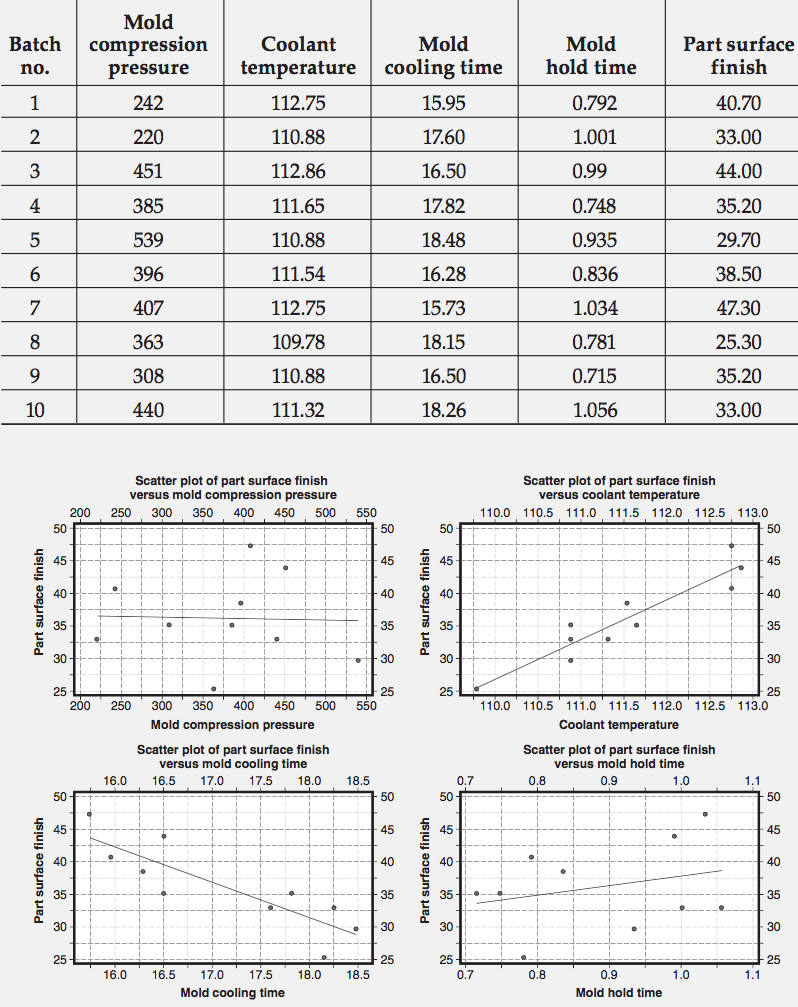
\includegraphics[width=150mm]{imagenes/ScatterDiagramsExamples.png}
	\caption{Scatter Diagrams Examples}
	\label{fig:ScatterDiagramsExamples}
\end{figure}

\subsubsection{Normal Probability Plots}

Sirve para comprobar si los datos vienen de una distribución normal. Hay varios tests para comprobar la normalidad:

\begin{itemize}
	\item Anderson-Darling test, basado en ECDF.
	\item El test Ryan-Joiner.
	\item El test Shapiro-Wilk, similar al Ryan-Joiner.
	\item El test Kolmogorov-Smirnov, basado en ECDF.
\end{itemize}

\subsubsection{Weibull Plots}

Es utilizada para la confianza de los datos cuando la distribución es desconocida. Puede ser utilizada para estimar la forma $\beta$ y el \textit{mean time between failures (MTBF)} o ratio de fallo.

\begin{equation}
P(x) = \alpha \beta (x-\gamma)^{\beta - 1}e^{-\alpha(x-\gamma)^\beta}
\end{equation}

Siendo $\alpha$ parámetro de escala, $\beta$ parámetro de forma y $\gamma$ parámetro de localización.

Las distribuciones Weibull con $\beta < 1$ tienen ratio decreciente con el tiempo, por ejemplo, mortalidad infantil. Los que tienen 1 o cercano a uno, la vida útil o fallo aleatorio, y con $\beta > 1$ tiene ratios de fallo que se incrementan con el tiempo.

\section{Measurement System Analysis}

El MSA es un area de estudios estadísticos que explora la variación de los datos en función de la \textit{Calibración}, \textit{Estabilidad}, \textit{Repetitividad}, \textit{Reproducibilidad}, \textit{Linealidad}, \textit{Sesgo}, \textit{Precisión} y \textit{Accuracy} (que es como precisión también).

Repetitividad: variación en el equipo de medida expresado en desviaciones estándar. 


Reproducibilidad: variación de la medida por el equipo de medición expresado en desviaciones estándar. 

GR\&R study
\begin{enumerate}
	\item Planifica el estudio en detalle comunicando a supervisor, asegurando el equipamiento para el estudio. Equipo calibrado y muestras en buenas condiciones... 
	\item Seleccionar e identificar las muestras. Cubrir el mayor espectro posible al seleccionarlas. 
	\item El siguiente paso es crear una tabla para anotar resultados de los experimentos.
	\item Cada medidor/tasador (persona) es llamado uno a uno y mide lo que se le pide según la hoja de experimentos.
	\item Se hacen las medias y el rango de las partes de cada uno. De entre todas las partes diferentes, se saca la media y el rango promedio. Esto tiene sentido para ver que con el mismo equipo de medida se están haciendo mediciones en torno a cierto valor y a cierto rango.
\end{enumerate}

\begin{figure}[ht!]
	\centering
	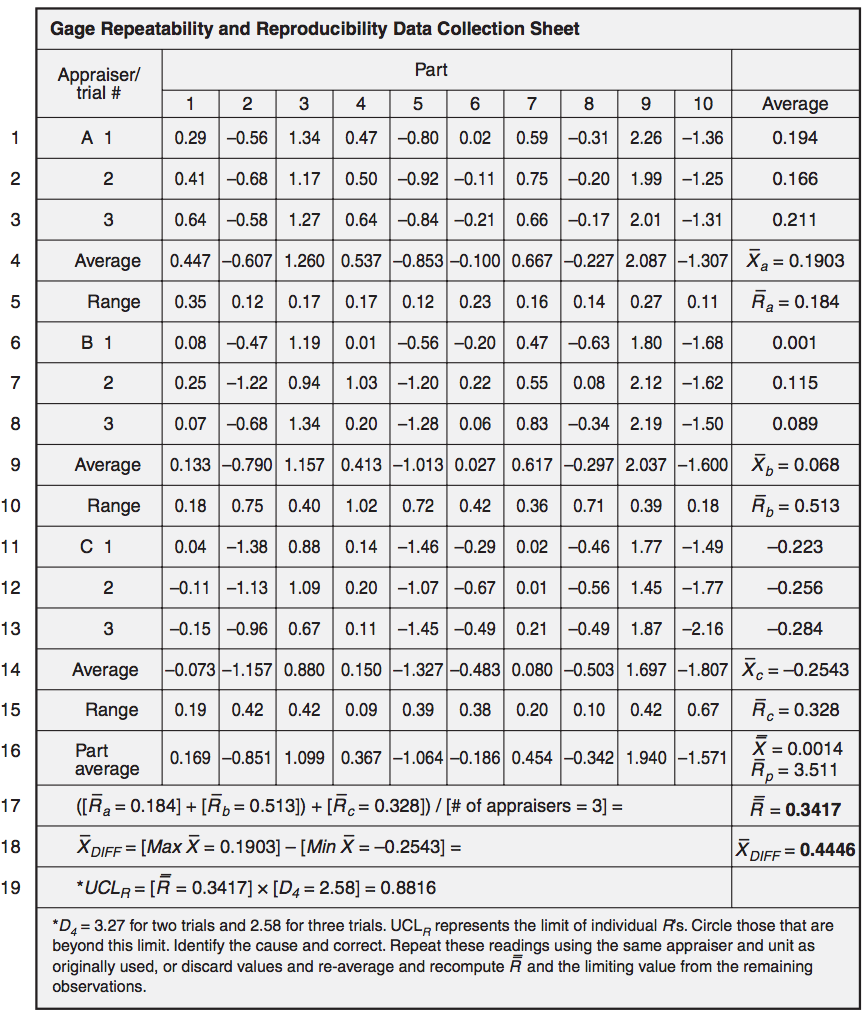
\includegraphics[width=150mm]{imagenes/GageRR.png}
	\caption{Gage R\&R}
	\label{fig:GageRR}
\end{figure}

\begin{figure}[ht!]
	\centering
	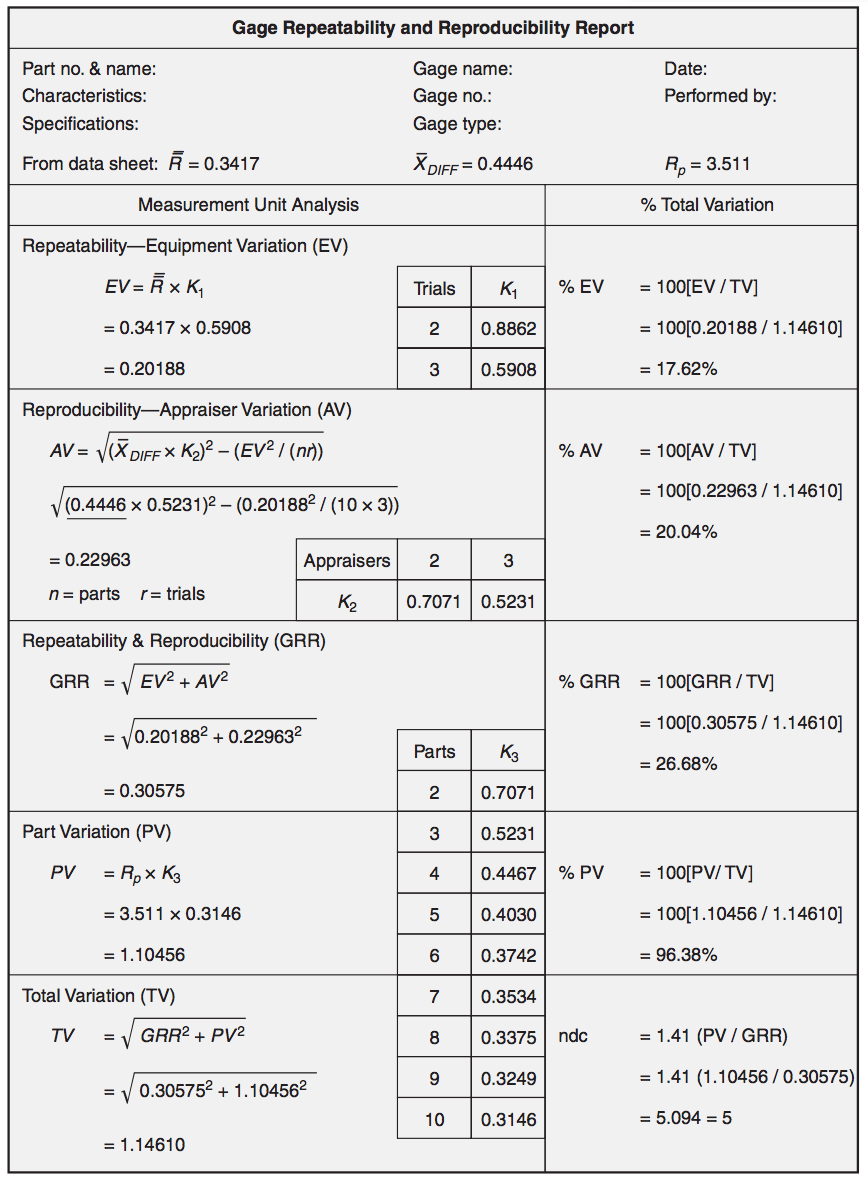
\includegraphics[width=150mm]{imagenes/GageRRReport.png}
	\caption{Gage R\&R Report}
	\label{fig:GageRRReport}
\end{figure}

\begin{figure}[ht!]
	\centering
	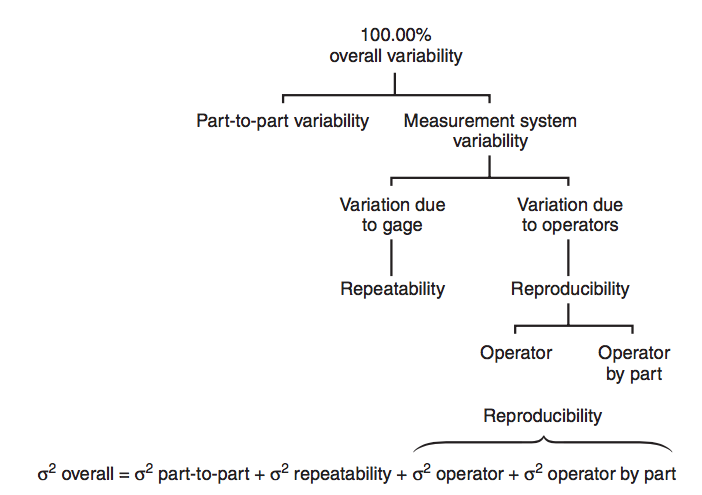
\includegraphics[width=150mm]{imagenes/Fuentesvariacionmedicion.png}
	\caption{Fuentes de variación de medición}
	\label{fig:Fuentesvariacionmedicion}
\end{figure}

Errores comunes durante la actuación del GR\&R:
\begin{itemize}
	\item No se seleccionan las muestras que pueden dar amplitud de resultados
	\item No se siguen un orden aleatorio a la hora de medir, sino que se sigue un orden.
	\item Utilizar appraisers (medidores) inexpertos o que habitualmente no miden lo que se está experimentando.
	\item Alterar las muestras durante le estudio (que se caigan al suelo, por ejemplo).
	\item Que el experimentador no esté presente durante el estudio R\&R.
	\item Publicar resultados con los nombres de las personas.
	\item Asumir que los resultados GR\&R son válidos para siempre.
	\item Asumir que la actuación GR\&R en una parte o pieza de un equipo es la misma para otro (equipo) del mismo tipo. Si cambia pieza, máquina que la fabrica, equipos utilizados para medir, o personas diferentes midiendo, el GR\&R es diferente.
\end{itemize}


\textbf{**** Este tema se queda incompleto ****} \newline 
\textbf{Hay que volver a él cuando termine con el resto} \newline
\textbf{***************************************} \newline

\pagebreak
\section{Process and Performance Capability}

\subsection{Process Performance Vs Process Specifitacions}

Define y distingue entre límites naturales de proceso y límites de especificación, calcular la metrología de la actuación del proceso.

Los límites de proceso naturales son calculados de la variación del proceso. Esto se hace a posteriori, cuando las causas especiales se han quitado y el proceso consigue una estabilidad estadística. Las especificaciones, son las expectativas de la ingeniería o del punto de vista del cliente. Cuando la variación del proceso es significativamente inferior a la amplitud de la especificación, es un proceso \textit{capable} (posible).

\begin{figure}[ht!]
	\centering
	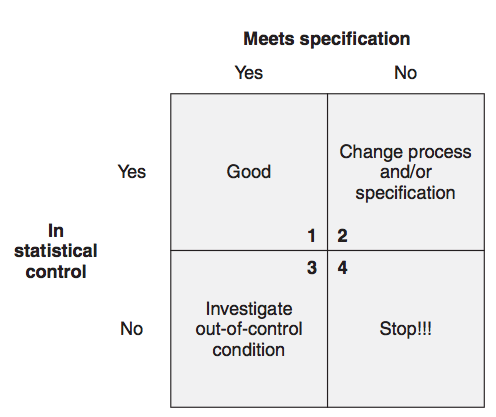
\includegraphics[width=90mm]{imagenes/Controllimitversusspecificationlimitgrid.png}
	\caption{Cuadro de control del límite vs límite de especificaciones}
	\label{fig:Controllimitversusspecificationlimitgrid}
\end{figure}

Un producto, después de ser empaquetado muestra que el peso está entre 1.00 y 1.10 kgs. Se recogen datos de 30 días de los envíos, y se determina que la distribución es normalmente distribuida y su control chart es estable. Control chart saca que el promedio es 1.065 kg, y el rango promedio en el que oscila es 0.05 ¿cual es el porcentaje de producto que puede estar siendo enviado con sobrepeso o bajopeso?

\begin{equation}
\sigma = \frac{R}{d_2} = \frac{0.05}{2.059} \approx 0.024 kg.
\end{equation}
El valor estadístico para la variable $d_2$ para un subgrupo de tamaño 4 es 2,059. USL/LSL = Upper/Lower Specification Limit, X = media del proceso y $\sigma$ = desviación estándar estimada:

\begin{equation}
Z_U = \frac{USL - X}{\sigma} = \frac{1.1 - 1.065}{0.024} = 1.46
\end{equation}

\begin{equation}
Z_L = \frac{X - LSL}{\sigma} = \frac{1.065 - 1}{0.024} = 2.7
\end{equation}

Sacando de la tabla los valores correspondientes a $Z_U$ = 1.46 y $Z_L$ = 2.7, tenemos que $\sigma_U$ = 0.0721, por lo que el 7.21\% de los envíos llevarán sobrepeso y tenemos $\sigma_L$ = 0.0035, por lo que el 0.35\% de los paquetes enviados estarán con el peso inferior.

La definición natural de límites de proceso es 3$\sigma$, en este caso 1.065 $\pm$ 3(0.024), [0.993 - 1.137].

\subsection{Process Capability Studies}

Define, describe y conduce las capacidades de un proceso, incluyendo la identificación de sus características, especificaciones, tolerancias y verificando la estabilidad y normalidad.

La \textit{Process capability} es la habilidad del proceso para tener las especificaciones esperadas. Cada proceso varía por causas comunes y especiales, internas y externas al proceso. Causas comunes: interacción entre pasos, diseño, variación natural por el material proporcionado, ..... Causas especiales: operadores con varios niveles de habilidad, cambios en la configuración del proceso, variaciones por el ambiente, cambios de equipo...

En la práctica la gente con experiencia en proceso normalmente puede identificar las características que necesita un estudio completo de \textit{capability}. En algunas industrias, los clientes identifican las características críticas que ellos necesitan. En la práctica con un FMEA se identifican los parámetros o características que necesitan un control estadístico de proceso y en base a esto se crea un planning SPC. 

En ocasiones, muchas veces se anuncian cosas tales como: Envío al día siguiente. Si la pizza tarda mas de 15 minutos, es gratis. 

\subsubsection{Steps for Process Capability Studies}

\begin{itemize}
	\item Verificación de sistemas de medición: una variación en el sistema de medición puede reducir la estabilidad de la monitorización del proceso. 
	\item Identificar el tamaño de los subgrupos para el control. Entre 2 y 10, mas de 5 no suele ser común. Mucho cuidado cuando hay menor variacion EN-o-DENTRO de subgrupos que entre subgrupos diferentes. Charts de desviación estandar promedio son usadas cuando el tamaño de grupo es mayor que 8.
	\item Estabilidad. Tras 20 puntos de subgrupos ploteados, si no hay causas especiales que se hayan mostrado, el proceso es considerado estable. Si 20 se antojan pocos, utilizar 30 o 40.
	\item La supervisión de la carta de control no se ve afectada, incluso si la distribución de los datos no es normal. Sin embargo, para medir la capacidad del proceso, la normalidad es necesaria para los datos continuos. \newline Para ello, construir un histograma usando las lecturas originales (no promedio). Con la mayoría de los puntos agrupados alrededor de un solo pico y con las caídas de la curva mas o menos simétricas a cada lado, se asume una población Normal.
	\item Si los datos procesados no están distribuidos bajo Normal, técnicas como transformación Box-Cox y transformaciones Johnson son utilizadas para transformación de datos no-normales.
\end{itemize}

El objetivo general del estudio de capacidad del proceso es monitorear si un proceso está en control estadístico y el proceso es capaz de cumplir con las especificaciones. Buscando que el proceso sea capaz, reducir la variación. Una posibilidad es revisar los límites entre Diseño, Ingeniería y Cliente. A veces los límites son reactualizables.

\subsubsection{Sampling with Respect to Statistical Process Control}

\begin{figure}[H]
	\centering
	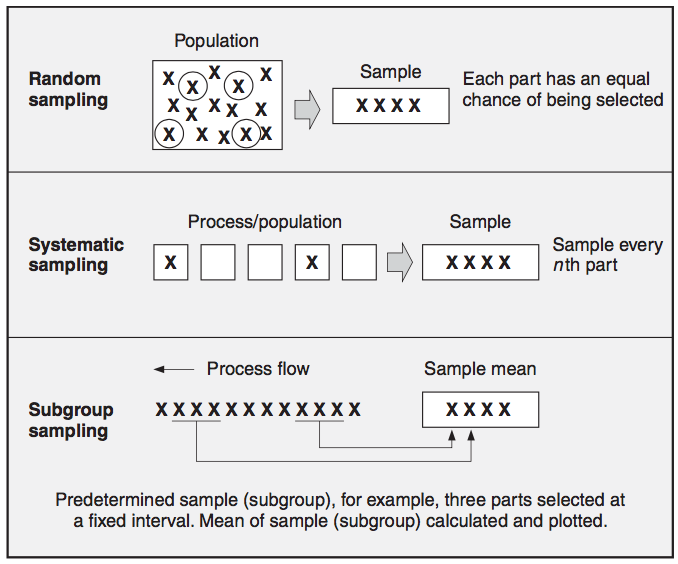
\includegraphics[width=120mm]{imagenes/SamplingSPC.png}
	\caption{Tipos de muestreo para el conjunto de datos del SPC}
	\label{fig:SamplingSPC}
\end{figure}


\subsection{Process Capability and Process Performance Indices}

\begin{equation}
C_{pk} = \frac{Min(Z_u,Z_L)}{3}
\end{equation}

Historicamente, un $C_{pk} > 1$ se considera \textit{capable}. $C_{pk} = 1.33$ 1.66 o 2 corressponde con $\pm$ 4$\sigma$, 5$\sigma$ o 6$\sigma$.

\begin{equation}
C_p = \frac{Tolerance zone}{6\sigma}
\end{equation}

La diferencia contra $C_pk$, es que $C_p$ no tiene en consideración si el proceso está centrado en la especificación. Muestra lo bueno que es un $C_pk$ si está centrado. La inversa de $C_p$ es $C_r$ y da en porcentaje la variación del proceso.

\subsubsection{Process Capability Calculations}

Dos cálculos son los que controlan e identifican lo capaz que es un proceso. Estos dos índices calculados son $C_p$ (índice de capacidad) y $C_{pk}$ (actuación del proceso).

Diferentes escenarios que nos encontramos: 
\begin{itemize}
	\item $C_p = 2$ y $C_{pk} = 1.5$ indican que el proceso está en Six Sigma.
	\item $C_p, C_{pk} \geq 1.3$ indican que el proceso es capaz.
	\item $C_p, C_{pk} = 1$ indica que el proceso cumple justo con las especificaciones. 0.27 unidades con defecto.
	\item $C_p, C_{pk} < 1$ fuera de especificaciones de ingeniería.
	\item $C_p, C_{pk} > 3$, valores anormalmente altos, la especificación es demasiado amplia o identifica la oportunidad de moverse hacia un proceso menos caro.
\end{itemize}

Interpretaciones sobre $C_p$ y $C_{pk}$:
\begin{itemize}
	\item Mayor $C_p$ y $C_{pk}$, mejor.
	\item El valor no cambia a medida que el proceso se centra en el objetivo a menos que algo en el proceso cambie.
	\item El valor de $C_p$ y $C_{pk}$ serán iguales si el proceso está centrado.
	\item $C_{pk}$ siempre es igual o menor a $C_p$
	\item Si $C_{pk}$ pasa a ser negativo, la media del proceso está fuera de alguna especificación de ingeniería.
\end{itemize}

\subsection{Short-Term vs Long-Term Capability and Sigma Shift}

Una línea de ensamblaje que envía unidades completas semanalmente muestrea aleatoriamente parámetros críticos en sus unidades. El ingeniero de calidad usa estos datos para medir índices de actuación para estos parámetros críticos. Desde que los datos incluyen variaciones a largo plazo y cambios, el ingeniero no debe utilizar las métricas $C_p$ y $C_{pk}$. Las medidas $C_p$ y $C_{pk}$ son usadas cuando la estabilidad del proceso es monitorizada a través de SPC y la desviación estandar se sale del rango principal. El ingeniero mide una desviación de 0,004 y una media de 10,014. Los límites de especificación son 9,99 y 10,03.

\begin{equation}
s = \sqrt{\frac{1}{N-1}\sum_{i=1}^{N}(x_i-x)^2} = 0.004
\end{equation}

\begin{equation}
P_p = \frac{Tolerancia}{6s} = \frac{10,03 - 9,99}{6*0,004} = 1.667
\end{equation}

\begin{equation}
P_{pk}= Min(\frac{USL - X}{3s}, \frac{X - LSL}{3s}) = Min(\frac{10,03-10,014}{3*0,004},\frac{10,014-9,99}{3*0,004})
\end{equation}

\begin{equation}
P_{pk} = Min(\frac{0,016}{0,012},\frac{0,024}{0,012})= Min(1.33 , 2) = 1.33
\end{equation}

Y ahora se compara el requerimiento contractual de los $P_p$ y $P_{pk}$ del cliente con los $P_p$ y $P_{pk}$ calculados.

Teniendo un proceso fuera de control se recomienda utilizar $P_p$ y $P_{pk}$, con la controversia de que es un proceso impredecible. Usar estos índices es un paso atrás, un gasto de energía e ingeniería y esfuerzo de gestión que no te lleva a nada.

\begin{equation}
C_{pm} = \frac{USL - LSL}{6 \sigma_{C_{pm}}}
\end{equation}

Indudablemente $C_p$ y $C_{pk}$ es una mejor medida que refleja lo capaz de un proceso.

$P_p$ y $P_{pk}$ pueden ser aplicados para recopilar datos de inspecciones de material para obtener una indicación de la actuación del proceso para el proveedor y donde los datos del SPC no están disponibles.

Dado que los datos del proceso pueden contener causas especiales, siempre que los datos sigan una distribución normal, $P_p$ y $P_{pk}$ pueden dar alguna idea sobre los procesos.

También es improbable que los proveedores implementados por el SPC estén dispuestos a compartir sus datos de proceso en secuencia temporal con sus clientes. Por lo tanto, $P_p$,
y $P_{pk}$ pueden servir de indicador para estas situaciones.

\subsubsection{Short-Term vs Long-Term Capability}

La \textit{Short-Term Capability} se calcula con datos recogidos de 20-30 subgrupos. La variabilidad es relativamente pequeña.

Para la \textit{Long-Term Capability} el muestreo se recoge atendiendo a diferentes procesos, cavidades, operarios, ... y teniendo en cuenta datos externos al proceso que pueden influir (temperatura, presión, número de equipos trabajando a la par, ...). Lo normal es que la variación del \textit{Long-Term} sea mayor que el \textit{Short-Term}.

Además, hay parámetros que no tienen que atender a distribuciones normales, como los tiempos de espera, por ejemplo. Técnicas de transformación de datos son utilizadas antes de analizar la capacidad de un proceso.

\begin{figure}[H]
	\centering
	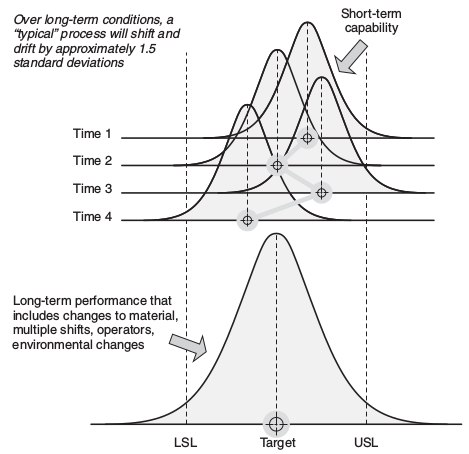
\includegraphics[width=120mm]{imagenes/ShortTermVsLongTerm.png}
	\caption{Variación del Short-Term y Long-Term.}
	\label{fig:ShortTermVsLongTerm}
\end{figure}

\part{Análisis}

\section{Exploratory Data Analysis}

\subsection{Estudios de multi-variable}

Selección de los planes apropiados de muestreo para crear cartas para el estudio multivariable e interpretar los resultados para la variación de posición, la variación de ciclo y la variación temporal.

\begin{tabular}{|c|c|c|}
	\hline Tipos de variación & Piezas & Lote \\ 
	\hline Posicional & Within-Part & Within-Lot \\ 
	\hline Cíclico & Part-to-part & Lot-to-Lot \\ 
	\hline Temporal & Over time (shift-to-shift) & Over time (shift-to-shift) \\ 
	\hline 
\end{tabular} 

Multi-var chart es útil para analizar los tres tipos de variación, también ayuda a minimizar la variación identificando áreas en las cuales hay una excesiva variación.
Posicional se refiere sobre las características en un mismo producto, cíclico es la variación sobre diferentes lotes y Temporal es la que ocurre con el paso del tiempo.


Procedimiento para un plan de muestreo multivariable

\begin{enumerate}
	\item Selección del proceso y de las características a ser investigadas,
	\item Selección de un tamaño de muestra gestionable, identificando en tiempo las muestras,
	\item Registrar tiempo y valores de cada muestra en un formato tabla,
	\item Representar un gráfico con el tiempo en la escala horizontal y los valores medidos en la vertical,
	\item Conectar los valores observados con líneas
	\item Observar y analizar la variación en la muestra, entre muestras, y a lo largo del tiempo,
	\item Focalizar estudios en las áreas donde haya máximas variaciones,
	\item Hacer mejoras de procesos y repetir estudios multivariable para confirmar los resultados.
\end{enumerate}

\subsection{Correlación y regresión lineal}

Correlación es encontrar la relación entre dos o más conjuntos de datos. Para encontrar correlación, tenemos que hablar de que hay una variable dependiente ($y$) y una independiente ($x$). Ejemplos. Horas estudiadas - Examen, Horas de ejercicio físico - Pérdida de peso, Cantidad de publicidad - Volumen de ventas.

\begin{figure}[H]
	\centering
	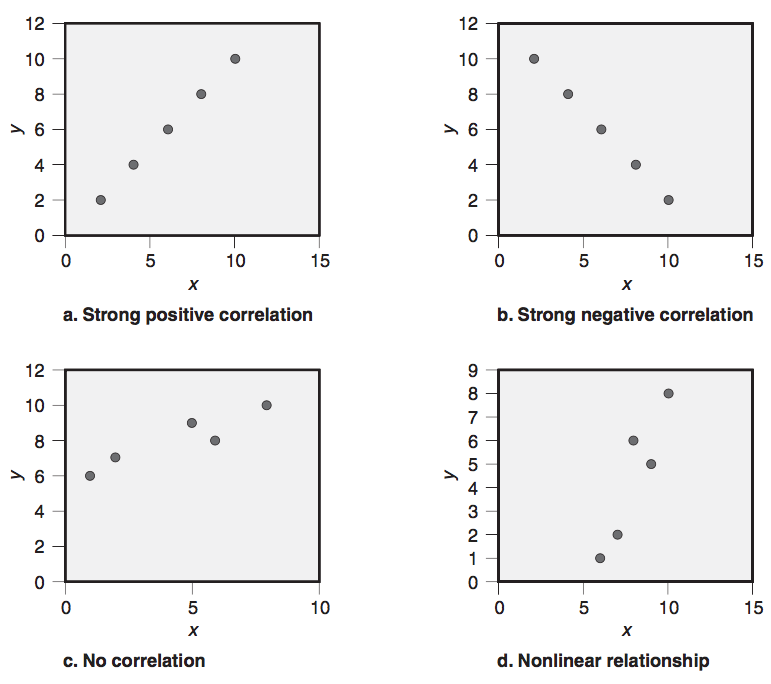
\includegraphics[width=120mm]{imagenes/Correlation.png}
	\caption{Correlation plot.}
	\label{fig:Correlation}
\end{figure}

\begin{equation}
r = \frac{1}{n-1} \sum \frac{(x-x_m)(y-y_m)}{S_xS_y}
\end{equation}

Procedimiento para calcular el coeficiente de correlación

\begin{enumerate}
	\item Calcular la media $x_m$ y $y_m$.
	\item Calcular desviaciones standart $S_x$ y $S_y$.
	\item Calcular la diferencia $x-x_m$ y $y-y_m$ para cada par de datos, y multiplicar las diferencias juntas
	\item Sumar todas las diferencias de producto. 
	\item Dividir la suma por el producto de las dos desviaciones estandar. 
	\item Dividir los resultados del paso anterior por $n-1$, siendo $n$ el número de parejas de datos (x,y)
\end{enumerate}

\subsubsection{p-valor}

P-valor es utilizado en el test de hipótesis para decidir cuando rechazar una hipótesis nula o no rechazarla. Es común utilizar 0.05 como p-valor. 

\begin{equation}
r = \frac{n*\Sigma xy - (x*y)}{\sqrt{(n*[\Sigma x^2- (\Sigma x)^2])(n*[\Sigma y^2- (\Sigma y)^2])}}
\end{equation}

\subsection{Regresión simple}

\begin{equation}
y = a + bx
\end{equation}

Siendo y el valor previsto, dado un valor de x. Siendo x la variable independiente.

\subsubsection{Procedimiento para Mínimos Cuadrados}

\begin{enumerate}
	\item Calcular xy, $x^2$ e $y^2$
	\item Calcular las sumas para x, y, xy, $x^2$, $y^2$, ademas de las medidas $x_m$ y $y_m$
	\item Encontrar la ecuación lineal que mejor se ajusta 
	\begin{equation}
	b = \frac{n \Sigma xy - (\Sigma x)(\Sigma y)}{n \Sigma x^2 - (\Sigma x)^2}
	\end{equation}
	\begin{equation}
		a = y - bx 
	\end{equation}
\end{enumerate}

\section{Hypotesis Testing}

\subsection{Términos básicos}

Una hipótesis es asumir un parámetro poblacional: el adulto promedio bebe 1.7 cafés al día.

Todos los test de hipótesis tienen hipótesis nula $H_0$ e hipótesis alternativa. $H_0$ significa que la media de la población es $\leq$, =, $\geq$ que un valor. $H_0$ es verdad si no se demuestra lo contrario. Una vez rechazada, la hipótesis alternativa debe ser considerada.

Un componente tiene un peso de 6 gramos. $\mu$ es la media poblacional. Hipótesis nula

\begin{equation}
H_0 : \mu = 6 \ , \ H_0 : \mu \leq 6 \ , \ H_0 : \mu \geq 6
\end{equation}

La hipótesis alternativa $H_1$ representa lo contrario a la $H_0$:

\begin{equation}
H_1 : \mu \neq 6 \ , \ H_1 : \mu < 6 \ , \ H_1 : \mu > 6
\end{equation}

\subsubsection{Tipos de Error}

\textit{Type I error}: resulta cuando la hipótesis nula es rechazada, siendo real.
\textit{Type II error}: resulta cuando la hipótesis nula no es rechazada, debiendo serlo.

\subsubsection{One-Tail Test}

Cuando hay algún riesgo asociado a él, y es asociado a $\alpha$ risk (type I error). El nivel del riesgo $\alpha$ determina el nivel de confianza que tenemos en la conclusión. Se utiliza para determinar le valor crítico del test estadístico.

Ejemplo: Una compañía inventa una pelota de golf que aumenta la distancia de lanzamiento en más de 20 metros. Test:  \newline \begin{center}
	$H_0$ : $\mu$ $leq$ 20, $H_1$ : $\mu$ > 20
\end{center}

Atendiendo a una campana de Gauss donde los extremos responden a la región de rechazo. Si la media de muestreo cae en la zona no-extremo, no rechazamos $H_0$. Esto es que no tenemos suficiente evidencia para apoyar $H_1$. Si la media de muestreo cae en la zona de rechazo, rechazamos $H_0$, esto significa que tenemos suficiente evidencia para apoyar $H_1$, y confirmamos que la bola incrementará su distancia en mas de 20 metros.

Muestras: 18, 20, 19, 18, 21, 19, 23, 18, 19, 22. \newline 
Test de $\mu$ = 20 vs $>$ 20. \newline
N: 10 ; Media: 19.7 ; StDev: 1.775 ; SE Mean: 0.561 ; 95\% Lower Bound: 18.644 ; T: -0.58 ; P: 0.713 \newline
p-value $>$ 0.05. La distancia adicional afirmada por la compañía no es estadísticamente válida.

\subsection{Test for Means, Variances and Proportions}

Para medias debe ser utilizado t-distribution:
\begin{equation}
X_m \pm t_{\alpha/2}\frac{s}{\sqrt{n}}
\end{equation}

\subsection{Student's t-Test}
\begin{equation}
t = \frac{X_m-\mu_0}{s/\sqrt{n}}
\end{equation}

\subsection{Intervalos de confianza para medias}
\begin{equation}
X_m \pm Z_{\alpha/2} \frac{\sigma}{\sqrt{n}}
\end{equation}

Ejemplo: Tenemos en cuenta un canal de compra. 32 clientes, con un pedido promedio en 78.25 euros, y la desviación 37.5 euros. ¿Cómo calculamos el intervalo de confianza al 95\% de la población? \newline
\begin{center}$\mu = 78.25 \pm 1.96\frac{37.50}{\sqrt{32}} = 78.25 \pm 13$ \end{center} 
\begin{center}$91.25 \geq \mu \geq 65.25 $ \end{center}

\section{Design of Experiments (DOE)}

Los DOE (\textit{Design of experiments}) puede ser resumido como un conjunto de experimentos planificados. Se ajustan el conjunto de variables bajo las condiciones controladas.

\textbf{Factor}: es la variable controlada por el experimentador, y puede ser visto como un estímulo.

\textbf{Levels}: un nivel refiere al ajuste o posibles valores de un valor en un diseño experimental (high-medium-low, por ejemplo).

\textbf{Treatment}: es un nivel simple asignado a un factor simple, durante el experimento, por ejemplo: presión 1 atmósfera.

\textbf{Block}: Es un etiqueta común a todos los elementos. Por ejemplo: muestras del mismo lote.

\textbf{Diseño experimental}: es el plan donde se incluyen las responsabilidades, factors, levels, treatments, blocks y el uso de la planificación y la replicación del experimento.

\textbf{Error experimental}: La variación en la variable de respuesta cuando los niveles y factores se mantienen constantes.

\textbf{Planned grouping}: La manera de buscar uniformidad en las muestras, en los \textit{Blocks}.

\textbf{Randomization}: Organiza el experimento para tener validez estadística.

\textbf{Replication}: incrementa precisión, reduce mediciones erróneas.

\textbf{Repetition}: Es el proceso para poder repetir el experimento con los mismos parámetros de máquina y sin encontrar variaciones.

\textbf{Variables}: Dependientes, independientes y de respuesta, que son las observadas como respuesta de un experimento.

\textbf{Effects}: Main effects e Interactions. Los efectos principales se definen como una estimación del efecto de un factor independiente de cualquier otro medio. Las interacciones ocurren cuando el efecto de un factor de entrada sobre el de salida depende del nivel de otro factor de entrada.

\subsubsection{DOE Overview}

\textbf{History of DOE}: Diseñar experimentos es un método estructurado y organizado que determina la relación entre factores (X's) que afectan a un proceso y el resultado del proceso (Y).

\textbf{Purpose}: El objetivo de diseñar un experimento es generar conocimiento sobre el producto o proceso. Se hace a través de: definir un objetivo, definir las variables que serán controladas, definir las variables que serán medidas para describir el resultado y examinar su precisión, y elegir el diseño que es compatible con el objetivo, numero de variables de diseño y precisión de medidas.

\textbf{Planning Test Programs}: Basado en la información de fondo, elegir los factores y el diseño del programa experimental. Clasificación:
\begin{itemize}
	\item \textit{Completamente aleatorios}: para cuando un solo factor es analizado
	\item \textit{Factorials}: apropiado cuando se investigan varios factores a dos o mas niveles y la interacción es necesaria.
	\item \textit{Blocked factorials}: reducen el número de ejecuciones y usa bloques para ejecutar experimentos en \textit{subsets}.
	\item textit{Fractional factorials}: reduce el número de combinaciones de factores y niveles requeridos para ser lanzado.
	\item \textit{Randomized blocks}: investigar un factor simple cuando el material puede ser bloqueado.
	\item ...
\end{itemize}
 
\textbf{Experimental Objectives}: \textit{¿Qué pregunta estamos intentando contestar?} 
\begin{itemize}
	\item Encontrar el procedimiento de inspección que dé mejor precisión.
	\item Encontrar el equilibrio entre emails y anuncios de TV que produce más ventas.
	\item Encontrar el recipiente de pastel que produce el sabor más consistente.
\end{itemize}
En cualquier caso, el objetivo debe ser medible, estar relacionado con metas y objetivos de la empresa y el sistema de medida que lo controle sea sencillo de manejar.

\subsubsection{DOE Design Principles}

\textit{Randomization}: Es un método de diseño y organización experimental que intenta disminuir los efectos de las variaciones por causas especiales. Ejemplo: 8 tratamientos diferentes, y se hacen 5 réplicas por tratamiento. El propósito de hacer los 40 tests es reducir la variación causada por \textit{variables ruido}.

\textit{Blocking}: intenta mitigar el efecto de variables que estamos intentando eliminar o evitar. Por ejemplo, los experimentos 1, 4, 5 y 8 se realizan durante el primer turno, y 2, 3, 6 y 7 durante el segundo.

\textit{Replication}: Es la repetición del conjunto de todas las combinaciones de tratamientos para ser comparadas en un experimento en orden aleatorio.

\textbf{Experimentation}: Un experimento planificado puede ser muy útil para entender la variación. El propósito de ejecutar un DOE es determinar los mejores caminos de hacer cosas o entender otros factores del proceso. Para cada prueba proceso/prueba/\textit{trial} se debe definir una lista de actividades. Un ejemplo de acciones que ayudan a tener un DOE con éxito: mapear el proceso, brainstorm de las causas de la variación, un diagrama causa-efecto, determinar los niveles de variación útiles dentro del proceso, definir el experimento, ejecutar el experimento operando el proceso usando factores varios, recoger muestras de cada experimento, calcular los factores que afectan, correr el proceso de nuevo para confirmar las mejoras, actualizar las plantillas de operaciones para mostrar los nuevos parámetros de operación.

Pasos prácticos importantes cuando se diseñan experimentos: comprobar los patrones y equipos de medición, hacer los experimentos lo más simples posibles, comprobar que todas las ejecuciones planificadas son factibles, evitar cambios no planeados, guardar algo de tiempo para eventos inesperados, guardar los datos en bruto, registrar todo lo que ocurra, resetear los equipos al terminar.

Los objetivos de experimento se pueden resumir en cuatro categorías: Comparatives (concluye si el factor es significante), Screening (selecciona unos pocos efectos principales), Response surface (encuentra la configuración óptima y los puntos débiles de los procesos) y Mixture.

Una vez configurados los objetivos los experimentos pueden ser desarrollados, lo mejor es utilizar pasos como: definir el objetivo, aprender echos sobre el proceso, hacer un brainstorm sobre variables dependientes e independientes, asignar niveles para las variables independientes, seleccionar o desarrollar un plan DOE, correr experimentos en orden aleatorio y analizar periódicamente, dibujar las conclusiones y verificar la replicación.

Tener en cuenta que para que el experimento sea válido hace falta que el sistema de medición sea capaz, que el proceso sea estable y que existen residuos y que éstos deben ser normalizados.

\textbf{Application of DOE}: Los operadores son los que conocen mejor las máquinas. A través de conocer cómo trabajan, se pueden tomar los parámetros de diseño y posteriormente, analizarlos bajo la óptica de la ingeniería para conseguir optimizar (rendimiento, las variables, tiempos, ...). Estos parámetros modificados deben ser verificados, saber si el equipo trabaja mejor en estas condiciones. Por ejemplo con SDCA (\textit{standarize, do, check, act}) es común mejorar los planes de control y las hojas de proceso.

\textbf{Simulation Studies}: Como el sofware de simulación incrementa la versatilidad y usabilidad de la simulación computerizada y la experimentación, se pueden conducir mas experimentos para mostrar potenciales resultados e interacciones. 

\begin{itemize}
	\item Especificar el problema, preguntas, necesidades del negocio y resultados esperados.
	\item Preparar un plan que incluya datos de prueba, colecciones de datos, escenarios alternativos, hitos y líneas temporales.
	\item Recoger datos, identificar vacíos.
	\item Construir un modelo que relacione inputs, las variables del proceso y outputs.
	\item Diseñar y ejecutar escenarios, distinguiendo entre parámetros variables y fijos, asegurando la reporoducibilidad de los resultados.
	\item Analizar e interpretar los datos, verificar las significancias estadísticas.
\end{itemize}

\subsection{Doe Graphs and Plots}
\subsubsection{Main Effects}
Son definidos como una estimación del efecto de un factor independiente de cualquier otro medio. El primer paso es calcular efectos principales, y son llamados \textit{average main effects}.

\subsubsection{Interaction Effects}
Las interacciones ocurren cuando el efecto de un factor de entrada sobre un factor de salida, depende del nivel de otro factor de entrada.

\begin{figure}[H]
	\centering
	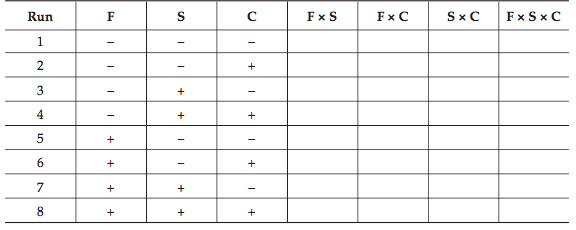
\includegraphics[width=90mm]{imagenes/a23design.png}
	\caption{$2^3$ full-factorial design.}
	\label{fig:A23design}
\end{figure}

\subsubsection{Balanced Designs}
Se llama \textit{Balanced} cuando cada configuración de factores aparece el mismo numero de veces que cada configuración de cada uno de los otros valores. \textbf{Es la mitad de un diseño $2^3$}.

\begin{figure}[H]
	\centering
	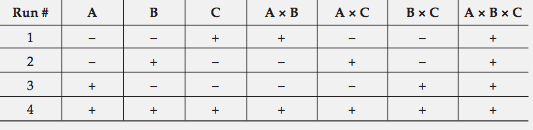
\includegraphics[width=80mm]{imagenes/a23halfdesign.png}
	\caption{$2^3$ half design.}
	\label{fig:a23halfdesign}
\end{figure}

\subsubsection{Effects and Confounding}

Un DOE utiliza los efectos para determinar si la configuración de un factor o no tiene impacto significativo en un proceso. 
Según la tabla \ref{fig:a23halfdesign}, la columna de la interacción A $\times$ B tiene la misma configuración que C. Esto significa que cuando el efecto C es calculado, no está claro si es debido al factor C o a la interacción A $\times$ B, o la combinación de ambas. Esto significa que el efecto de C está \textit{confounded} con la interacción A $\times$ B.

\subsubsection{Diseño y análisis de experimentos de un factor}
Experimentos de un factor son aleatorios cuando no hay pruebas omitidas y el orden es completamente aleatorio. Los resultados son analizados y evaluados con ANOVA y los valores significantes exceden el F-statistic.
\subsubsection{Diseño y análisis de Full Factorial Experiments}
Buscan todas las posibilidades de combinación de factores para completar un estudio de interacciones. Pueden ser mantenidas y convertidas en diferentes diseños de experimentos. A través de un two-way ANOVA se comprueba si son estadísticamente significativos.

Ejemplo: Estas cocinando carne para 100 personas y el ratio de aceptabilidad es del 75\%. Quieres saber el efecto de diferentes métodos de cocinar y las aproximaciones para ver como afecta.
Método: + es grill, - es frito. Carne: + es solomillo, - es costilla. Marinado: + es vino rojo, - es salsa de soja.

\begin{table}[H]
	\begin{center}
\begin{tabular}{|c|c|c|c|c|}
	\hline Experimento & Método & Carne & Marinado & \% de aprobado \\ 
	\hline 1 & - & - & - & 66 \\ 
	\hline 2 & + & - & - & 88 \\ 
	\hline 3 & - & + & - & 58 \\ 
	\hline 4 & + & + & - & 84 \\ 
	\hline 5 & - & - & + & 67 \\ 
	\hline 6 & + & - & + & 91 \\ 
	\hline 7 & - & + & + & 63 \\ 
	\hline 8 & + & + & + & 84 \\ 
	\hline 
\end{tabular} 
		\caption{Tabla 1 de ejemplo de ejercicio Full Factorial Experiment.}
		\end{center}
\end{table}

Método: [(88+84+91+84)-(66+58+67+63)]/4 = 23.25 \newline
Carne: [(58+84+63+84)-(66+88+67+91)]/4 = -5.75 \newline
Marinado: [(67+91+63+84)-(66+88+58+84)] = 2.25


\begin{table}[H]
	\begin{center}
		\begin{tabular}{|c|c|c|c|p{1.5cm}|p{1.5cm}|p{1.5cm}|p{1.8cm}|c|}
			\hline Experimento & Método & Carne & Marinado & Cook $\times$ Meat & Meat $\times$ Mar & Cook $\times$ Mar & Cook $\times$ Meat $\times$ Mar & \% de aprobado \\ 
			\hline 1 & - & - & - & + & + & + & - & 66 \\ 
			\hline 2 & + & - & - & - & + & - & + & 88 \\ 
			\hline 3 & - & + & - & - & - & + & + & 58 \\ 
			\hline 4 & + & + & - & + & - & - & - & 84 \\ 
			\hline 5 & - & - & + & + & - & - & + & 67 \\ 
			\hline 6 & + & - & + & - & - & + & - & 91 \\ 
			\hline 7 & - & + & + & - & + & - & - & 63 \\ 
			\hline 8 & + & + & + & + & + & + & + & 84 \\ 
			\hline 
		\end{tabular} 
		\caption{Tabla 2 de ejemplo de ejercicio Full Factorial Experiment.}
	\end{center}
\end{table}

Método y Carne: [(66+84+67+84)-(88+58+91+63)]/4 = 1.25
Carne y Marinado: [(66+88+63+84)-(58+84+67+91)]/4 = 0.25
Método y Marinado: [(66+58+91+84)-(88+84+67+63)]/4 = -0.75
Método, Carne y Marinado [(88+58+67+84)-(66+84+91+63)] = -1.75

Las interacciones tiene mínimos efectos en cuanto a la aprobación o retirada. La conclusión es que el método (grill o frito) tiene mayor efecto que el resto.

\subsubsection{Diseño y análisis de experimentos de Two-Level Fractional Factorial}
\begin{equation}
Number of runs = L^F
\end{equation}
Siendo L el número de niveles, y F el número de factores.

\begin{table}[H]
	\begin{center}
		\begin{tabular}{|c|c|c|c|c|}
			\hline Experimento & Método & Carne & Marinado & \% de aprobado \\ 
			\hline 2 & + & - & - & 88 \\ 
			\hline 3 & - & + & - & 58 \\ 
			\hline 5 & - & - & + & 67 \\ 
			\hline 8 & + & + & + & 84 \\ 
			\hline 
		\end{tabular} 
		\caption{Tabla de ejemplo de ejercicio Fractional Factorial Experiment.}
	\end{center}
\end{table}

Método: [(88+84)-(58+67)]/2 = 23.5
Carne: [(54+84)-(88+67)]/2 = -6.5
Marinado: [(67+84)-(88+58)]/2 = 2.5

Aunque los resultados no son iguales que en el caso anterior, las conclusiones son similares.

\subsubsection{Two-Level Fractional Factorial Experiment Procedure}

El procedimiento se resume en tres etapas: seleccionar un proceso, seleccionar un diseño y analizar los datos-dibujar las conclusiones.

Ejemplo:
Selecciona un proceso e identifica inputs y outputs.
\begin{enumerate}
	\item Desarrollo y entrega de software a un cliente
	\item El éxito se basa en el despliegue sin problemas críticos que requieren resoluciones de alta prioridad
	\item Estudiar el efecto de siete variables en dos niveles.
\end{enumerate}

\begin{table}[H]
	\begin{center}
\begin{tabular}{|p{5cm}|p{5cm}|p{5cm}|}
	\hline Input factors & Level 1 (-) & Level 2 (+) \\
	\hline A. Requisitos & 20 requsitos de alto nivel & Definir +400 requisitos \\
	\hline B. Analisis de riesgo & Minimal checklist & Formal \\
	\hline C. Arquitectura & Agil & Estructurada \\
	\hline D. Diseño y código & Prototipo & Etapa consensuada \\
	\hline E. Integración de sistema & Freeware y Shareware & Componentes precualificados \\
	\hline F. Test de producto & Explicar y checks aleatorios & Unidad-integración-sistema-usuario \\
	\hline G. Aseguramiento de Calidad & Inspección final & Series de 5 pasa no pasa para aprobar \\
	\hline
\end{tabular}
\end{center}
\end{table}
Experimento: Siete factores se evaluan a dos niveles. \textit{Pass} es que no tiene problemas críticos. \textit{Score} es satisfacción de cliente.

\begin{table}[H]
	\begin{center}
\begin{tabular}{|c|c|c|c|c|c|c|c|c|c|}
	\hline Test & A & B & C & D & E & F & G & Pass & Score \\
	\hline 1 & + & + & - & + & - & - & + & Yes+& 85 \\
	\hline 2 & + & + & - & - & + & + & - & No- & 57 \\
	\hline 3 & + & - & + & + & - & + & - & No- & 82 \\
	\hline 4 & + & - & + & - & + & - & + & Yes+& 100 \\
	\hline 5 & - & + & + & + & + & - & - & No- & 69 \\
	\hline 6 & - & + & + & - & - & + & + & Yes+& 87 \\
	\hline 7 & - & - & - & + & + & + & + & No- & 72 \\
	\hline 8 & - & - & - & - & - & - & - & No- & 44 \\
	\hline
\end{tabular}
\end{center}
\end{table}


\begin{table}[H]
	\begin{center}
		\begin{tabular}{|c|c|c|c|c|c|c|c|c|c|}
			\hline Test & A & B & C & D & E & F & G & Pass & Score \\
			\hline 1 & +85 & +85 & -85 & +85 & -85 & -85 & +85 & Yes+& 85 \\
			\hline 2 & +57 & +57 & -57 & -57 & +57 & +57 & -57 & No- & 57 \\
			\hline 3 & +82 & -82 & +82 & +82 & -82 & +82 & -82 & No- & 82 \\
			\hline 4 & +100 & -100 & +10 & -100 & +100 & -100 & +100 & Yes+& 100 \\
			\hline 5 & -69 & +69 & +69 & +69 & +69 & -69 & -69 & No- & 69 \\
			\hline 6 & -87 & +87 & +87 & -87 & -87 & +87 & +87 & Yes+& 87 \\
			\hline 7 & -72 & -72 & -72 & +72 & +72& +72 & +72 & No- & 72 \\
			\hline 8 & -44 & -44 & -44 & -44 & -44 & -44 & -44 & No- & 44 \\
			\hline 
			\hline Difference ($\Sigma_1^8$) & 52 & 0 & 80 & 20 & 0 & 0 & 92 &  &  \\
			\hline Effect (/4) & 13 & 0 & 20 & 5 & 0 & 0 & 23 & & \\
			\hline
		\end{tabular}
	\end{center}
\end{table}

Los grandes contribuidores son C (arquitectura) y G (aseguramiento de la calidad).

\subsection{DOE Considerations}

\begin{itemize}
	\item Trabajar con expertos en la materia para determinar que factores deben ser incluidos en el experimento.
	\item Evaluar el proceso histórico para especificar los valores de cada factor.
	\item Determinar los factores representativos y sus niveles
	\item Usar registros históricos para revisar datos existentes y determinar cuantos más datos adicionales deben ser recogidos para obtener confianza estadística.
\end{itemize}

\section{Root Cause Analysis}

El enfoque de las ocho disciplinas (8D): \begin{enumerate}
	\item Utilizar enfoque de equipo. Junta a quien conoce el proceso y tiene habilidades técnicas para resolver el problema. Asigna un campeón que conduzca al equipo.
	\item Describe el problema. Usa técnicas de calidad y métodos para describir el problema y el impacto en el objetivo. Ayuda a priorizar sobre los objetivos y acciones.
	\item Empieza y comprueba acciones internas. 
	\item Define y comprueba las causas raíz. Haz pruebas, aísla otras causas/parámetros. Asegura que la causa raíz es la que genera el problema.
	\item Comprobar acciones correctivas. Confirma si las acciones correctivas se están llevando a cabo adecuadamente.
	\item Empieza acciones correctivas permanentes. 
	\item Evitar problemas futuros. Las modificaciones que es hagan deben evitar que los problemas sean recurrentes de cara al futuro.
	\item Felicitar al equipo. Dar reconocimiento.
\end{enumerate}

\subsection{Fase 1: Identificar la oportunidad (Problem Identification)}
Las oportunidades para la mejora deben ser identificadas y priorizadas atendiendo al equipo y el alcance. Métodos para identificar los problemas: 
\begin{itemize}
	\item Análisis Pareto: campos de fallo, quejas, retornos, basura, reworks, ...
	\item Propuestas de esquemas de sugerencia, 
	\item Necesidades de los usuarios/empleados, \textit{feedback} del mercado, ...
	\item Resultados de auditorías y observaciones,
	\item Encuestas a clientes, empleados y stakeholders,
	\item Brainstorming, 
\end{itemize}
Tres atributos deben estar presentes para que un problema sea seleccionado y priorizado:
\begin{itemize}
	\item Divergencia significativa respecto a los estandares generales,
	\item Inconsistentes impresiones y objetivo evidente,
	\item Causa raíz no identificada,
\end{itemize}
Criterios para seleccionar:
\begin{itemize}
	\item El problema es importante y sustancial. ¿Por qué?
	\item ¿Resolver el problema ayuda al logro de objetivos?
	\item ¿Puede el problema ser definido usando mediciones objetivas?
\end{itemize}

\subsection{Fase 2: Analizar el proceso actual}
En esta fase los límites del proceso son definidos especificando los \textit{outputs} y clientes, los \textit{inputs} y proveedores y el flujo de proceso. Los niveles de satisfacción de cliente y medidas necesidades para permitir la recolección de datos y la identificación de la causa raíz. Hay que desarrollar los procesos atendiendo a: 
\begin{itemize}
	\item Líneas de actuación de acuerdo a los requisitos del cliente
	\item Datos necesitados para gestionar el proceso
	\item Feedback de clientes y proveedores
	\item Calidad/coste/líneas temporales de \textit{inputs} y \textit{outputs}.
\end{itemize}
Ventajas de recoger datos: confirmar problemas y hechos, tener criterio sobre las magnitudes y la posibilidad de medir los resultados una vez.

El método más efectivo para esta fase es el diagrama causa-efecto.
Procedimiento:
\begin{enumerate}
	\item Examinar la causa más probable de los problemas.
	\item Validar los datos para la causa mas probable.
	\item Distinguir que elementos del proceso cambian entre estado controlado y fallo.
	\item Someter la causa a escrutinio.
	\item Usar diseño experimental, Taguchi, y otras técnicas avanzadas para determinar factores críticos y sus niveles.
	\item Confirmar con datos durante los pasos de verificación.
\end{enumerate}

\subsection{Fase 3: Desarrollar las soluciones óptimas (correcciones)}
Al obtener la información, el equipo del proyecto comienza su búsqueda de posibles soluciones. La creatividad y la lluvia de ideas sobre posibles soluciones requieren la creación, combinación o modificación de prácticas existentes. La combinación de dos o más procesos es una actividad de síntesis que depende en gran medida del \textit{benchmarking}.
Una vez que se han determinado las soluciones posibles, la evaluación o la prueba de las soluciones viene a continuación. Los criterios de aceptación incluyen cosas tales como costo, factibilidad, efecto, resistencia al cambio, consecuencias y entrenamiento. Las soluciones deben evitar la recurrencia y resolver el problema.

\subsection{Fase 4: Implementar cambios}
Los cambios se implementan usando un plan que describa las 5W1H: \textit{who, what, when, where, why, how}. Incluye responsabilidades, horarios, hitos y la monitarización de actividades. Herramientas de medida como \textit{run charts, control charts, Pareto, histogramas, ...}

\subsection{Fase 5: Estudiar los resultados}
A través de los datos recogidos, se puede conocer cuán significativo es el cambio y la mejora puede ser lograda. Evaluando los resultados el equipo puede verificar y validar que el problema ha sido resuelto o determinar si hay otros problemas que han surgido a través del desarrollo de la solución.

\subsection{Fase 6: Estandarizar la solución}
\textit{Positrol} (control positivo) asegura que las variables importantes están bajo control, especifica las 5W1H del proceso y es una actualización de la solución. Estandarizarla evita el que la solución retroceda. Los operadores necesitan claras instrucciones para los procesos particulares, \textit{training} para asegurar el proceso y conocimiento sobre el proceso que le sigue, por lo que un conocimiento completo del producto es deseable.

\subsection{Fase 7: Plan para el futuro}
Habitualmente hay que planificar revisiones del progreso para identificar las mejoras futuras. Se tiene que ir controlando los cambios en las necesidades del cliente

\subsection{Root Cause Analysis Methodology}
El \textit{Root Cause Analysis} (RCA) es la metodología para analizar un problema y poner la solución para que el problema no vuelva a repetirse nunca más. Problem-solving y RCA es el corazón del proceso \textit{corrective and preventive action} (CAPA).
Metodología de actuación RCA:
\begin{enumerate}
	\item Define y documenta el problema que requiere RCA.
	\item Entiende el problema.
	\item Consigue datos y analízalos.
	\item Determina la causa raíz. 
	\item Establece un programa de acciones correctivas.
	\item Implementa el plan de acciones correctivas.
	\item Evalúa los efectos de la implementación para demostrar que la causa raíz del problema fue eliminada.
\end{enumerate}
Para encontrar las causas: análisis de valor añadido, comparación de procesos \textit{as-is} vs \textit{should-be}, FMEA, análisis de cambio-evaluación, de errores en prevención o de predicción.

\subsection{Identificando la causa raíz}

El diagrama Cause-and-Effect o Ishikawa/Fishbone diagram identifica todas las causas probables y las selecciona para investigar. La construcción del diagrama CE:
\begin{enumerate}
	\item Crear un equipo de individuos que conozcan el proceso, los problemas y otras funciones
	\item Definir el problema (efecto). Ponerlo en el extremo derecho y dibujar una flecha que apunte hasta él.
	\item Lluvia de ideas y listar todas las posibles causas.
	\item Agrupar las causas en categorías y darle a cada una un nombre.
	\item Dibujar el diagrama con líneas al estilo \textit{fishbone}.
	\item Asignar las causas de las ideas en las categorías.
	\item Redondear las causas más posibles. El equipo tiene que agrupar información para verificar la causa mas probable.
\end{enumerate}
Maneras de agrupar: \begin{itemize}
	\item Man - Machine - Material - Method - Maintenance - Management - Measurement - Mother Nature.
	\item Product - Place - People - Process - Promotion - Productivity - Price - Physical evidence
	\item Suppliers - Systems - Surroundings - Skills
\end{itemize}
El diagrama \textit{fishbone} se utiliza junto con los \textbf{5 why's} para conseguir llegar a la raíz de los problemas.

\subsubsection{5 Whys}
Consiste en preguntar 5 veces ¿por qué? consiguiendo entrar en detalle cada vez más para conocer cual es la raíz de un problema.

\subsubsection{Cause-and-Effect Relational Matrix}
Es una matriz para cuantificar y priorizar los impactos de causas (X) en efectos (Y) a través de un ranking numérico. 

\begin{figure}[H]
	\centering
	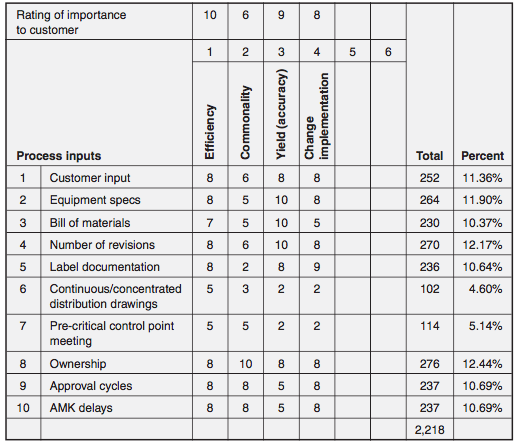
\includegraphics[width=80mm]{imagenes/Cause-and-effectrelationalmatrix.png}
	\caption{Cause-and-effect relational matrix.}
	\label{fig:Cause-and-effectrelationalmatrix}
\end{figure}


\subsubsection{Root Cause tree}
Diagrama para ver visualmente la conexión entre efectos por fallos y la causa potencial y problemas centrales.

\begin{figure}[H]
	\centering
	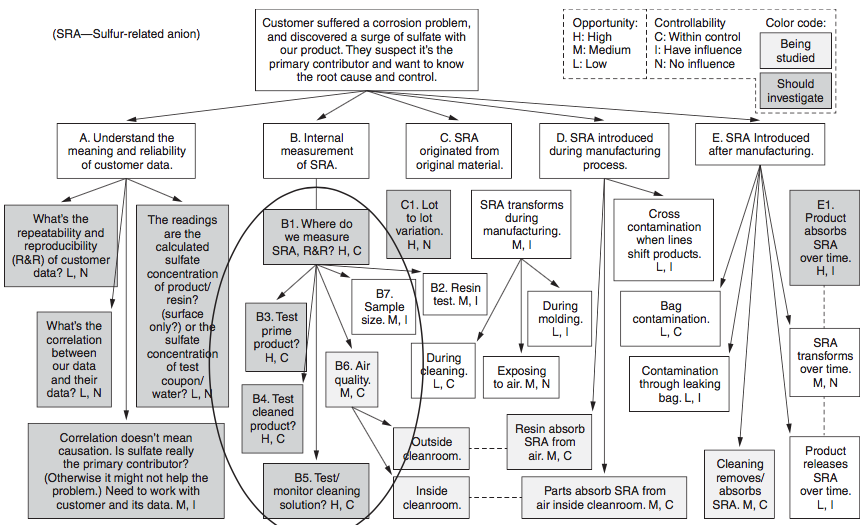
\includegraphics[width=140mm]{imagenes/Rootcausetreeexample.png}
	\caption{Root cause tree example.}
	\label{fig:Rootcausetreeexample}
\end{figure}

\subsection{Failure Mode and Effects Analysis}
Es un grupo de actividades para reconocer y evaluar los fallos potenciales de un producto o proceso e identificar los efectos de tal fallo, identificar las acciones para eliminar o reducir la posibilidad de que ocurran, documentar el proceso entero.

El propósito de un FMEA es entender la oportunidad para fallos y el impacto de los riesgos en un producto o proceso, priorizar riesgos, tomar acciones para eliminar o reducir el impacto de los riesgos.

\section{Lean Tools}
El objetivo es alcanzar mejoras en la actuación y la filosofía Lean Six Sigma abordará eficazmente las medidas clave de actuación, la identificación y actuación, los múltiples aspectos sobre la gestión de procesos, incluyendo diseño, mejora y control, así como las mejoras a través de múltiples áreas de manera transversal, incorporando metas financieras, presupuestos y revisiones en el \textit{Framework} de mejora.

\begin{figure}[H]
	\centering
	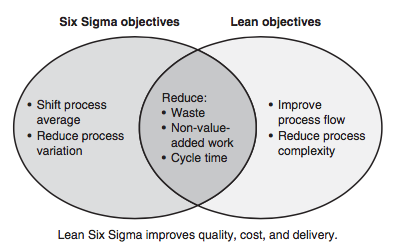
\includegraphics[width=80mm]{imagenes/LeanSixSigmaObjectives.png}
	\caption{Lean Six Sigma Objectives.}
	\label{fig:LeanSixSigmaObjectives}
\end{figure}

\begin{figure}[H]
	\centering
	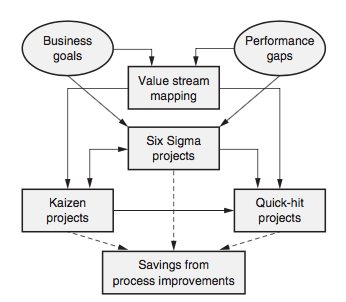
\includegraphics[width=70mm]{imagenes/ProjectFramework.png}
	\caption{Project Framework.}
	\label{fig:ProjectFramework}
\end{figure}

\subsubsection{Lean vs sistema tradicionales}

\begin{center}
\textit{Diseño del producto o servicio} - \textit{Capacidad} - \textit{System Layout} - \textit{Workforce} - \textit{Scheduling} - \textit{Inventarios} - \textit{Suppliers} - \textit{Operaciones}
\end{center}
\subsection{Waste Elimination}
\subsubsection{Ejemplos de herramientas Lean}
Uno de los problemas principales en todas las organizaciones es el control de los procesos. Además de las técnicas \textit{statistical process control} (SPC), un GB debe utilizar las herramientas que están catalogadas como \textit{Lean Thinking}. Hay que identificar el valor en términos de cada producto específico atendiendo a su \textit{value stream}, hacer un \textit{value flow} sin interrupción o retrasos, permitir al cliente añadir valor a través de los pasos del proceso, perseguir la perfección y evitar el \textit{rework}.

Lean es la aplicación de herramientas para quitar \textit{waste} y variación en un proceso, en el ámbito de herramientas de control: 5S, \textit{Visual factory}, \textit{Kaizen}, \textit{Kanban}, \textit{Poka-yoke}, \textit{Total productive maintenance}, \textit{Standard work}, \textit{Pull systems}.

\paragraph{Pull system}

Se encarga de gestionar el calendario y el flujo de materiales para qu no exista sobre producción o exceso de inventario. Este sistema está conducido por la demanda del cliente e incorpora métricas del proceso (\textit{setup time, takt time, ...}) para determinar tiempos y cantidades. Operan con \textit{Little's law} que definen la relación entre \textit{Lead time, throughput} y \textit{work-in-process} (WIP). Reduciendo inventario WIP, se reducen \textit{Lead times}, resultando más rápida la entrega y la satisfacción de la demanda del cliente.

Eficiencias: simplificación, centrado en minimizar tiempos para setups y cambios, reducción de pasos, eliminación de \textit{reworks}, gestión de cuellos de botella.

\paragraph{Visual Factory}

Se esfuerza en hacer los problemas visibles, notificar a los empleados las condiciones del trabajo (herramientas, parámetros, etc..) y las metas de los procesos (5000 uds, hasta las 12...) a través de \textit{production and schedule boards}.

\paragraph{Kaizen}
Es la mejora continua. El control de procesos puede ser mejorado a través de eventos \textit{Kaizen} y recomendaciones para evitar actividades que no dan valor añadido. El trabajo resultante es más productivo y permite centrarse en los procesos necesarios.

\paragraph{Kanban}
Un sistema \textit{Kanban} bien implementado, mejora el sistema de control asegurando los tiempos de movimientos, la información, asegurando los flujos de material dentro y fuera del proceso de manera suave. Si al proceso llegan los \textit{inputs} antes de necesitarlos o hay una confusión innecesaria, empiezan a haber costes. Si los \textit{outputs} no están sincronizados con los procesos siguientes, los resultados son retrasos, clientes cabreados, y costes asociados.

\paragraph{Total Productive Maintenance}

Conlleva las siguientes iniciativas: \begin{itemize}
	\item Evitar reducir o parar la actuación por equipo roto.
	\item Reducir y minimizar los tiempos por setups y cambios.
	\item Evitar paradas por procesar productos o servicios inaceptables.
	\item Asegurar que los equipos producen a la velocidad para la que fueron diseñados.
	\item Incrementar el campo de materiales aceptables para reducir \textit{waste}, \textit{scrap}, \textit{rework}...
\end{itemize}

\paragraph{Standard Work}
Es un término para describir de manera sistemática como las partes son procesas e incluye las interacciones hombre-máquina. Encontrar la mejor manera de producir un producto cada vez más consistente es la esencia del control del proceso.

\subsection{Cycle-time Reduction}

\paragraph{Standard Work}
El \textit{Standar Work} establece la línea de base para realizar tareas y actividades para obtener el resultado deseado, enlazando con la calidad del producto y proceso, costo, programación, ejecución, tiempo de ciclo y satisfacción del cliente. Se pueden demostrar mejoras en la calidad y el tiempo de ciclo y las reducciones en los residuos (por ejemplo, eliminación del exceso de movimiento, chatarra y \textit{rework}) con respecto a la línea de base.

El \textit{Standar Work} se establece mediante el análisis, la observación y la participación de los empleados. Los empleados están involucrados porque las personas más cercanas a la obra lo entienden mejor. Cabe señalar que los empleados pueden ser resistentes al establecimiento de trabajos estándar. El uso de herramientas de calidad y de gestión ayuda a evaluar las posibles barreras mediante el análisis y / o la participación del equipo en la siguiente secuencia:

\begin{enumerate}
	\item Comunicar el cambio
	\item Identificar los beneficios
	\item Identificar las barreras
	\item Identificar como capitalizar los beneficios
	\item Identificar los métodos para mitigar las barreras
	\item Hacer un acuerdo entre los pasos 4 y 5
	\item Implementar el cambio
	\item Comunicar los resultados
	\item Celebrar el éxito
\end{enumerate}

Beneficios: proceso estable, proceso claramente definido, aprendizaje organizacional, participación de los trabajadores, siembra la base para aplicar Lean (por ejemplo: poka-yoke).

\begin{itemize}
	\item Production Capacity Chart. Usado para determinar la capacidad de máquinas y humanos en un proceso. Su propósito es identificar cuellos de botellas dentro del proceso. La clave es: capacidad, tiempo de proceso, intervalo, setup, tiempo operacional por cambio.
	\item Standarized Work Combination Table. Muestra los elementos de trabajo y su secuencia. La tabla debe incluir las interacciones entre operador y máquina, y máquinas entre sí. Se utiliza para detectar actividades que no dan valor añadido.
	\item Standarized Work Analysis Chart. Usado como racionalización de un layout de proceso. Es una ayuda visual a un empleado que esté en proceso de aprendizaje. Incluye localización de las cosas, pasos, y tiempos. También recalca items de calidad y seguridad.
\end{itemize}

\paragraph{SIPOC}

Un \textit{Chart} SIPOC ofrece un enfoque centrado en el cliente, simplificando el proceso de conocer sobre como se organiza todo en una compañía, mostrando las relaciones e interdependencias entre procesos y departamentos.

\paragraph{Process Stability}
Procesos estables tienen costes, calidad y ciclos precedibles. Alternativamente, sin estabilidad la planificación se hace difícil. Para lograr estabilidad:
\begin{itemize}
	\item Method. Pasos claros y de consecución.
	\item People. Niveles mínimos de \textit{training} y cualificación.
	\item Machinery. Diseñada y mantenida en un método consistente.
	\item Measurement. El equipo es utilizado adecuadamente, mantenido y regularmente calibrado.
	\item Materials. Calidad consistente.
\end{itemize}

\paragraph{Process Capability}
Es similar a \textit{voice of the customer} (VOC), serí como el \textit{voice of the process} (VOP).

\paragraph{Process Capacity}
Herramienta para calcular la capacidad de un equipo para un trabajo particular. Las variables a utilizar: tiempo de máquina por pieza, tiempo manual (de operador) por pieza, ciclo total por pieza, número de piezas antes de cambiar las herramientas (mantenimiento), tiempo requerido para realizar un cambio de herramienta, ...

\paragraph{Work Flow Analysis}
El \textit{Work Flow} es el ratio bajo el que el trabajo es procesado a través del sistema.

\textit{Flowcharting} es la técnica para representar visualmente una secuencia ordenada de tareas. El \textit{flowchart} puede ser construido a partir de una lista de tareas e incluye todo lo relevante del proceso (inputs, outputs, puntso de decisión, tiempos, métricas, ...)

Pasos para el análisis:
\begin{enumerate}
	\item Processing. Cambio físico en el material.
	\item Inspection. Comparación con el estándar.
	\item Transportation. Movimiento entre localizaciones.
	\item Process delay. Tiempo desde que se empieza a producir hasta que el lote es procesado.
	\item Lot delay. Utilizado para representar la situación donde una pieza es procesada mientras otras piezas del lote esperan ser inspeccionadas o transportadas.
\end{enumerate}

\textbf{Value Stream Mapping} identifica las actividades que dan valor y las que crean desperdicios. Permite visualizar los flujos de productos, servicios e información, los desperdicios y sus fuentes, así como niveles y funciones. Su uso ayuda a tomar decisiones sobre flujo de procesos, a mejorar la estrategia y sobre las relaciones entre información y los flujos de producto.

\textit{Current State}. Observar la información y dibujar el \textit{VSM} reuniendo: tiempos de ciclo, tiempos de cambios, número de personas, \textit{uptime/downtime}, \textit{work-in-process}, inventario, tamaño de packaging, ratio de defectos, tiempo total operativo, tiempo de valor añadido vs tiempo de valor no añadido, \textit{Lead time}, número de cambios.

\textit{Future State}. Brainstorming de ideas para mejorar el estado actual del \textit{VSM}.

\textit{Establish and Implement a Plan}. Crear un plan de acción para alcanzar el plan futuro.

\textbf{Takt Time Analysis}. El tiempo existente entre completar unidades consecutivas.
\begin{equation}
Takt \ time = \frac{Tiempo \ disponible \ de \ trabajo}{Demanda \ de \ cliente} (sobre \ un \ periodo \ de \ tiempo)
\end{equation}
Ejemplo: Un turno de 8 horas tiene 480 minutos. Un proceso de pintura de una fábrica necesita pintar 160 piezas al día para cumplir con la demanda del cliente. El \textit{takt time} promedio es 3 minutos por unidad. Por lo tanto, el \textit{flow rate} por paso debe ser menor o igual a 3 minutos por proceso.

\subsection{Kaizen and Kaizen Blitz}

\textit{Kaizen} es mejora continua. Permite progreso a través de generación de ideas, pruebas y fases de evaluación. 

\textit{Kaizen Blitz} incorpora \textit{workshops} y eventos, incluyendo a equipos transversalmente funcionales para completar un proyecto conjunto en una semana.

\paragraph{Kaikaku}

Es la innovación. Ya que las mejoras de \textit{Kaizen} son pequeñas y las modificaciones van estabilizando el proceso, \textit{kaizen} puede ser descrito como \textit{evolutionary}. 

\textit{Kaikaku} se refiere a una acción Kkaizen centrada para resolver una actividad concreta en una semana, referida como \textit{kaizen blitz} o \textit{kaizen event}. Las mejoras \textit{kaikaku} pueden deteriorarse en el tiempo si no hay nadie que las controle constantemente y resuelva los pequeños problemas.

\textit{Gemba} es definida como el lugar donde el trabajo ocurre. Los esfuerzos \textit{kaizen} son condizidos en el Gemba por estos operadores e individuos que conocen el proceso de mejor manera. Para llevar a cabo un \textit{gemba kaizen}, los miembros de equipos utilizan un checklist para economizar los movimientos que incluyen:

\begin{enumerate}
	\item Eliminar movimientos innecesarios.
	\item Reducir movimientos de ojos.
	\item Combinar operaciones.
	\item Mejorar el lugar de trabajo.
	\item Mejorar herramientas y máquinas.
\end{enumerate}

Las directrices de \textit{gemba kaizen} incluyen los objetivos del proyecto, calendario, actividades principales y abarcan:
\begin{enumerate}
	\item Seleccionar el \textit{target}.
	\item Seleccionar los líderes.
	\item Confirmar la linea operativa.
	\item Confirmar el inventario.
	\item Explicar el propósito del proyecto.
	\item Preparar herramientas.
	\item Seleccionar planes \textit{kaizen}.
	\item Instruir los operadores.
	\item Preparar estándares.
	\item Preparar el informe de resultados.
\end{enumerate}

Para el éxito del plan:
\begin{itemize}
	\item Seleccionar el reto con objetivos bien definidos.
	\item Hacer equipos transversales para solucionar los problemas.
	\item Tomar acciones con velocidad.
	\item Invertir tiempo en preparar, comunicar y planificar el trabajo.
	\item Plantear como objetivo \textit{kaizen} la transferencia de aprendizaje y habilidades.
\end{itemize}

\paragraph{Organizing for Kaizen}

Hay muchos niveles de mejora para actividades kaizen, con diferente alcance y profundidad.
\begin{itemize}
	\item Individual (point kaizen). A nivel individual de estacioon de trabajo, siempre hay oportunidades para reducir desechos, organización del trabajo, inventario, localización de herramientas, secuencia de trabajo, ergonomía, poka-yoke, ...
	\item Work teams (mini kaizen). Equipos de trabajo toman proyectos de mejora afectando al area de trabajo colectivo. Work flow, balanceo de carga de trabajo, 5S, mejoras en calidad.
	\item Flow kaizen. Dirigido por un Project Manager, a menudo asistido por un \textit{Champion}, y asesorado por consultores, el equipo es multidisciplinar. Los flujos de los proyectos kaizen tratan cuestiones de proceso, de sistema y organizativas. 
	\item Process kaizen. Centrado en la eliminación de \textit{waste}, focalizado en un proceso-subproceso específico.
	\item Supply chain kaizen. Los equipos de proyectos de la cadena de suministro implican a las empresas participantes en el flujo de valor en centrarse en optimizar las mejoras de la cadena de suministro. Estos equipos suelen tener un gerente de proyecto, por lo general de la empresa fabricante de equipos originales (OEM), y son apoyados por los campeones y consultores.
\end{itemize}

\paragraph{Kaizen Events}
Mientras que \textit{blitz} se refiere a un equipo específico que intenta conseguir rápidamente optimizar y reconstruir procesos para funcionar de manera eficiente, kaizen se utiliza para todos los tipos de mejora. Principios kaizen para una perspectiva lean:
\begin{itemize}
	\item Definir el valor percibido por el cliente
	\item Identificar el Value Stream
	\item Eliminar waste
	\item Crear flujo
	\item Establecer donde el flujo no es posible
	\item Perseguir la perfección
\end{itemize}
Enfoque:
\begin{itemize}
	\item Kaizen es trabajo de todos
	\item "Ir al \textit{Gemba}", para observar y documentar la realidad
	\item Enfasis en los problemas que preocupan
	\item Usar herramientas problema-solución
	\item Sesgar a la hora de actuar
	\item Estandarizar una vez que la mejora se ha logrado
	\item Focalizar en mejorar procesos y resultados a la vez
	\item Aplicar a cualquier aspecto del trabajo
\end{itemize}
Aspectos para lograr el éxito:
\begin{itemize}
	\item Charter. Establece el marco, determina el problema, miembros, recursos, como las mejoras van a ser medidas.
	\item Identificación de factores críticos de éxito. Elementos críticos para el proceso deben ser identificados, definidos y medidos.
	\item Alcance. Saber hasta donde se llega en cada actuación.
	\item Enlazar evento \textit{kaizen} con plan de negocio. Alinear esfuerzos con las metas de la organización.
	\item Seleccionar equipo. Capacidades y habilidades, expertos en el proceso, ...
	\item \textit{Follow-through}. Buen \textit{follow-through} es necesario para segurar que las mejoras son mantenidas y evitar volver atrás.
	\item Presentar resultados. 
	\item Visibilidad. Quien no esté envuelto en esto debe también conocer las mejoras que está haciendo el equipo.
	\item Comité de gestión. La dirección debe apoyar activamente y participar en las iniciativas kaizen. Debe asegurar que el equipo tiene todo lo que necesita.
\end{itemize}
%\pagebreak[4]
%\part{Glosario}

%Una relación de palabras y traducciones Español - Inglés de cara al examen:

%Skills - Habilidades. Relativas al conocimiento o técnica.
%Reliability - Confianza/Confiabilidad. Relativo a los datos.
%Appraiser - Medidor/Tasador. Relativo a personas.

\end{document}
